\documentclass[twoside]{book}

% Packages required by doxygen
\usepackage{fixltx2e}
\usepackage{calc}
\usepackage{doxygen}
\usepackage[export]{adjustbox} % also loads graphicx
\usepackage{graphicx}
\usepackage[utf8]{inputenc}
\usepackage{makeidx}
\usepackage{multicol}
\usepackage{multirow}
\PassOptionsToPackage{warn}{textcomp}
\usepackage{textcomp}
\usepackage[nointegrals]{wasysym}
\usepackage[table]{xcolor}

% Font selection
\usepackage[T1]{fontenc}
\usepackage[scaled=.90]{helvet}
\usepackage{courier}
\usepackage{amssymb}
\usepackage{sectsty}
\renewcommand{\familydefault}{\sfdefault}
\allsectionsfont{%
  \fontseries{bc}\selectfont%
  \color{darkgray}%
}
\renewcommand{\DoxyLabelFont}{%
  \fontseries{bc}\selectfont%
  \color{darkgray}%
}
\newcommand{\+}{\discretionary{\mbox{\scriptsize$\hookleftarrow$}}{}{}}

% Page & text layout
\usepackage{geometry}
\geometry{%
  a4paper,%
  top=2.5cm,%
  bottom=2.5cm,%
  left=2.5cm,%
  right=2.5cm%
}
\tolerance=750
\hfuzz=15pt
\hbadness=750
\setlength{\emergencystretch}{15pt}
\setlength{\parindent}{0cm}
\setlength{\parskip}{3ex plus 2ex minus 2ex}
\makeatletter
\renewcommand{\paragraph}{%
  \@startsection{paragraph}{4}{0ex}{-1.0ex}{1.0ex}{%
    \normalfont\normalsize\bfseries\SS@parafont%
  }%
}
\renewcommand{\subparagraph}{%
  \@startsection{subparagraph}{5}{0ex}{-1.0ex}{1.0ex}{%
    \normalfont\normalsize\bfseries\SS@subparafont%
  }%
}
\makeatother

% Headers & footers
\usepackage{fancyhdr}
\pagestyle{fancyplain}
\fancyhead[LE]{\fancyplain{}{\bfseries\thepage}}
\fancyhead[CE]{\fancyplain{}{}}
\fancyhead[RE]{\fancyplain{}{\bfseries\leftmark}}
\fancyhead[LO]{\fancyplain{}{\bfseries\rightmark}}
\fancyhead[CO]{\fancyplain{}{}}
\fancyhead[RO]{\fancyplain{}{\bfseries\thepage}}
\fancyfoot[LE]{\fancyplain{}{}}
\fancyfoot[CE]{\fancyplain{}{}}
\fancyfoot[RE]{\fancyplain{}{\bfseries\scriptsize Generated by Doxygen }}
\fancyfoot[LO]{\fancyplain{}{\bfseries\scriptsize Generated by Doxygen }}
\fancyfoot[CO]{\fancyplain{}{}}
\fancyfoot[RO]{\fancyplain{}{}}
\renewcommand{\footrulewidth}{0.4pt}
\renewcommand{\chaptermark}[1]{%
  \markboth{#1}{}%
}
\renewcommand{\sectionmark}[1]{%
  \markright{\thesection\ #1}%
}

% Indices & bibliography
\usepackage{natbib}
\usepackage[titles]{tocloft}
\setcounter{tocdepth}{3}
\setcounter{secnumdepth}{5}
\makeindex

% Hyperlinks (required, but should be loaded last)
\usepackage{ifpdf}
\ifpdf
  \usepackage[pdftex,pagebackref=true]{hyperref}
\else
  \usepackage[ps2pdf,pagebackref=true]{hyperref}
\fi
\hypersetup{%
  colorlinks=true,%
  linkcolor=blue,%
  citecolor=blue,%
  unicode%
}

% Custom commands
\newcommand{\clearemptydoublepage}{%
  \newpage{\pagestyle{empty}\cleardoublepage}%
}

\usepackage{caption}
\captionsetup{labelsep=space,justification=centering,font={bf},singlelinecheck=off,skip=4pt,position=top}

%===== C O N T E N T S =====

\begin{document}

% Titlepage & ToC
\hypersetup{pageanchor=false,
             bookmarksnumbered=true,
             pdfencoding=unicode
            }
\pagenumbering{alph}
\begin{titlepage}
\vspace*{7cm}
\begin{center}%
{\Large Final-\/\+Project-\/\+Group9 \\[1ex]\large 2.\+o }\\
\vspace*{1cm}
{\large Generated by Doxygen 1.8.13}\\
\end{center}
\end{titlepage}
\clearemptydoublepage
\pagenumbering{roman}
\tableofcontents
\clearemptydoublepage
\pagenumbering{arabic}
\hypersetup{pageanchor=true}

%--- Begin generated contents ---
\chapter{Namespace Index}
\section{Namespace List}
Here is a list of all namespaces with brief descriptions\+:\begin{DoxyCompactList}
\item\contentsline{section}{\hyperlink{namespacefp}{fp} \\*Namespace from the base class }{\pageref{namespacefp}}{}
\end{DoxyCompactList}

\chapter{Hierarchical Index}
\section{Class Hierarchy}
This inheritance list is sorted roughly, but not completely, alphabetically\+:\begin{DoxyCompactList}
\item \contentsline{section}{fp\+:\+:Algorithm}{\pageref{classfp_1_1_algorithm}}{}
\item \contentsline{section}{fp\+:\+:A\+PI}{\pageref{classfp_1_1_a_p_i}}{}
\item \contentsline{section}{fp\+:\+:Land\+Based\+Robot}{\pageref{classfp_1_1_land_based_robot}}{}
\begin{DoxyCompactList}
\item \contentsline{section}{fp\+:\+:Land\+Based\+Tracked}{\pageref{classfp_1_1_land_based_tracked}}{}
\item \contentsline{section}{fp\+:\+:Land\+Based\+Wheeled}{\pageref{classfp_1_1_land_based_wheeled}}{}
\end{DoxyCompactList}
\item \contentsline{section}{Landbased\+Robot}{\pageref{class_landbased_robot}}{}
\item \contentsline{section}{fp\+:\+:Maze}{\pageref{classfp_1_1_maze}}{}
\end{DoxyCompactList}

\chapter{Class Index}
\section{Class List}
Here are the classes, structs, unions and interfaces with brief descriptions\+:\begin{DoxyCompactList}
\item\contentsline{section}{\hyperlink{classfp_1_1_algorithm}{fp\+::\+Algorithm} }{\pageref{classfp_1_1_algorithm}}{}
\item\contentsline{section}{\hyperlink{classfp_1_1_a_p_i}{fp\+::\+A\+PI} }{\pageref{classfp_1_1_a_p_i}}{}
\item\contentsline{section}{\hyperlink{classfp_1_1_land_based_robot}{fp\+::\+Land\+Based\+Robot} }{\pageref{classfp_1_1_land_based_robot}}{}
\item\contentsline{section}{\hyperlink{class_landbased_robot}{Landbased\+Robot} }{\pageref{class_landbased_robot}}{}
\item\contentsline{section}{\hyperlink{classfp_1_1_land_based_tracked}{fp\+::\+Land\+Based\+Tracked} \\*A Landbased\+Tracked class. }{\pageref{classfp_1_1_land_based_tracked}}{}
\item\contentsline{section}{\hyperlink{classfp_1_1_land_based_wheeled}{fp\+::\+Land\+Based\+Wheeled} \\*A Landbased\+Wheeled class. }{\pageref{classfp_1_1_land_based_wheeled}}{}
\item\contentsline{section}{\hyperlink{classfp_1_1_maze}{fp\+::\+Maze} }{\pageref{classfp_1_1_maze}}{}
\end{DoxyCompactList}

\chapter{File Index}
\section{File List}
Here is a list of all files with brief descriptions\+:\begin{DoxyCompactList}
\item\contentsline{section}{\hyperlink{main_8cpp}{main.\+cpp} }{\pageref{main_8cpp}}{}
\item\contentsline{section}{src/\+Algorithm/\hyperlink{_algorithm_8cpp}{Algorithm.\+cpp} }{\pageref{_algorithm_8cpp}}{}
\item\contentsline{section}{src/\+Algorithm/\hyperlink{_algorithm_8h}{Algorithm.\+h} \\*Class to be used in source file and the functions that have been used }{\pageref{_algorithm_8h}}{}
\item\contentsline{section}{src/\+A\+P\+I/\hyperlink{api_8cpp}{api.\+cpp} }{\pageref{api_8cpp}}{}
\item\contentsline{section}{src/\+A\+P\+I/\hyperlink{api_8h}{api.\+h} \\*Class to be used in source file and the functions that have been used }{\pageref{api_8h}}{}
\item\contentsline{section}{src/\+Land\+Based\+Robot/\hyperlink{_land_based_robot_8cpp}{Land\+Based\+Robot.\+cpp} }{\pageref{_land_based_robot_8cpp}}{}
\item\contentsline{section}{src/\+Land\+Based\+Robot/\hyperlink{_land_based_robot_8h}{Land\+Based\+Robot.\+h} \\*A file for base class inclusion }{\pageref{_land_based_robot_8h}}{}
\item\contentsline{section}{src/\+Land\+Based\+Tracked/\hyperlink{_land_based_tracked_8cpp}{Land\+Based\+Tracked.\+cpp} }{\pageref{_land_based_tracked_8cpp}}{}
\item\contentsline{section}{src/\+Land\+Based\+Tracked/\hyperlink{_land_based_tracked_8h}{Land\+Based\+Tracked.\+h} \\*A file for base class inclusion }{\pageref{_land_based_tracked_8h}}{}
\item\contentsline{section}{src/\+Land\+Based\+Wheeled/\hyperlink{_land_based_wheeled_8cpp}{Land\+Based\+Wheeled.\+cpp} }{\pageref{_land_based_wheeled_8cpp}}{}
\item\contentsline{section}{src/\+Land\+Based\+Wheeled/\hyperlink{_land_based_wheeled_8h}{Land\+Based\+Wheeled.\+h} \\*A file for base class inclusion }{\pageref{_land_based_wheeled_8h}}{}
\item\contentsline{section}{src/\+Maze/\hyperlink{_m_a_z_e_8cpp}{M\+A\+Z\+E.\+cpp} }{\pageref{_m_a_z_e_8cpp}}{}
\item\contentsline{section}{src/\+Maze/\hyperlink{_m_a_z_e_8h}{M\+A\+Z\+E.\+h} \\*Class declarartion with functions wrapped in the namespace fp }{\pageref{_m_a_z_e_8h}}{}
\end{DoxyCompactList}

\chapter{Namespace Documentation}
\hypertarget{namespacefp}{}\section{fp Namespace Reference}
\label{namespacefp}\index{fp@{fp}}


namespace from the base class  


\subsection*{Classes}
\begin{DoxyCompactItemize}
\item 
class \hyperlink{classfp_1_1_algorithm}{Algorithm}
\item 
class \hyperlink{classfp_1_1_a_p_i}{A\+PI}
\item 
class \hyperlink{classfp_1_1_land_based_robot}{Land\+Based\+Robot}
\item 
class \hyperlink{classfp_1_1_land_based_tracked}{Land\+Based\+Tracked}
\begin{DoxyCompactList}\small\item\em A Landbased\+Tracked class.. \end{DoxyCompactList}\item 
class \hyperlink{classfp_1_1_land_based_wheeled}{Land\+Based\+Wheeled}
\begin{DoxyCompactList}\small\item\em A Landbased\+Wheeled class.. \end{DoxyCompactList}\item 
class \hyperlink{classfp_1_1_maze}{Maze}
\end{DoxyCompactItemize}


\subsection{Detailed Description}
namespace from the base class 

This namespace is used for convience and avoid conflict with std. 
\chapter{Class Documentation}
\hypertarget{classfp_1_1_algorithm}{}\section{fp\+:\+:Algorithm Class Reference}
\label{classfp_1_1_algorithm}\index{fp\+::\+Algorithm@{fp\+::\+Algorithm}}


{\ttfamily \#include $<$Algorithm.\+h$>$}

\subsection*{Public Member Functions}
\begin{DoxyCompactItemize}
\item 
bool \hyperlink{classfp_1_1_algorithm_aa7083be9be18b81bedf9bcc9976e97af}{if\+\_\+visited} (std\+::pair$<$ std\+::pair$<$ int, int $>$, char $>$ new\+\_\+node)
\begin{DoxyCompactList}\small\item\em a function to check wether we have visited nodes or not. \end{DoxyCompactList}\item 
bool \hyperlink{classfp_1_1_algorithm_a92571327e87248eb1afc706d571e47e0}{if\+\_\+duplicated} (std\+::pair$<$ std\+::pair$<$ int, int $>$, char $>$ new\+\_\+state)
\begin{DoxyCompactList}\small\item\em a function to check wether we have duplicate state in new node \end{DoxyCompactList}\item 
bool \hyperlink{classfp_1_1_algorithm_a2e66300e1507ff3f71d5fbbffede52a3}{Solve} (std\+::shared\+\_\+ptr$<$ \hyperlink{classfp_1_1_land_based_robot}{fp\+::\+Land\+Based\+Robot} $>$, \hyperlink{classfp_1_1_maze}{fp\+::\+Maze} \&)
\begin{DoxyCompactList}\small\item\em function is the gist of B\+FS \hyperlink{classfp_1_1_algorithm}{Algorithm}. \end{DoxyCompactList}\item 
bool \hyperlink{classfp_1_1_algorithm_a237fc28eed2899786cd06f4e5a0e7333}{is\+Goal} (int x, int y)
\begin{DoxyCompactList}\small\item\em a function to check wether we have visited nodes or not. \end{DoxyCompactList}\end{DoxyCompactItemize}


\subsection{Detailed Description}
\begin{DoxyAuthor}{Author}
Group-\/9-\/\+E\+N\+P\+M809Y 
\end{DoxyAuthor}
\begin{DoxyDate}{Date}
03/12/19 
\end{DoxyDate}


\subsection{Member Function Documentation}
\mbox{\Hypertarget{classfp_1_1_algorithm_a92571327e87248eb1afc706d571e47e0}\label{classfp_1_1_algorithm_a92571327e87248eb1afc706d571e47e0}} 
\index{fp\+::\+Algorithm@{fp\+::\+Algorithm}!if\+\_\+duplicated@{if\+\_\+duplicated}}
\index{if\+\_\+duplicated@{if\+\_\+duplicated}!fp\+::\+Algorithm@{fp\+::\+Algorithm}}
\subsubsection{\texorpdfstring{if\+\_\+duplicated()}{if\_duplicated()}}
{\footnotesize\ttfamily bool fp\+::\+Algorithm\+::if\+\_\+duplicated (\begin{DoxyParamCaption}\item[{std\+::pair$<$ std\+::pair$<$ int, int $>$, char $>$}]{new\+\_\+state }\end{DoxyParamCaption})}



a function to check wether we have duplicate state in new node 

a function to check wether we are in new or visited state.


\begin{DoxyParams}{Parameters}
{\em a} & 2-\/D vector of new state \\
\hline
\end{DoxyParams}
\begin{DoxyReturn}{Returns}
True or False 
\end{DoxyReturn}
\hypertarget{_m_a_z_e_8h_DESCRIPTION}{}\subsection{D\+E\+S\+C\+R\+I\+P\+T\+I\+ON}\label{_m_a_z_e_8h_DESCRIPTION}
A function is basically comparing co-\/ordinates of x-\/y coordinates with previous node to new node and if we have visted then set to false or else set true. Here is the caller graph for this function\+:
\nopagebreak
\begin{figure}[H]
\begin{center}
\leavevmode
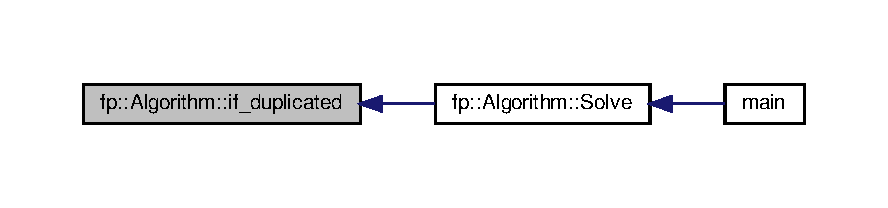
\includegraphics[width=350pt]{classfp_1_1_algorithm_a92571327e87248eb1afc706d571e47e0_icgraph}
\end{center}
\end{figure}
\mbox{\Hypertarget{classfp_1_1_algorithm_aa7083be9be18b81bedf9bcc9976e97af}\label{classfp_1_1_algorithm_aa7083be9be18b81bedf9bcc9976e97af}} 
\index{fp\+::\+Algorithm@{fp\+::\+Algorithm}!if\+\_\+visited@{if\+\_\+visited}}
\index{if\+\_\+visited@{if\+\_\+visited}!fp\+::\+Algorithm@{fp\+::\+Algorithm}}
\subsubsection{\texorpdfstring{if\+\_\+visited()}{if\_visited()}}
{\footnotesize\ttfamily bool fp\+::\+Algorithm\+::if\+\_\+visited (\begin{DoxyParamCaption}\item[{std\+::pair$<$ std\+::pair$<$ int, int $>$, char $>$}]{new\+\_\+state }\end{DoxyParamCaption})}



a function to check wether we have visited nodes or not. 

a function to check if we are in new node during visiting or not.


\begin{DoxyParams}{Parameters}
{\em a} & 2-\/D vector of new state \\
\hline
\end{DoxyParams}
\begin{DoxyReturn}{Returns}
True or False 
\end{DoxyReturn}
\hypertarget{_m_a_z_e_8h_DESCRIPTION}{}\subsection{D\+E\+S\+C\+R\+I\+P\+T\+I\+ON}\label{_m_a_z_e_8h_DESCRIPTION}
A function is basically comparing co-\/ordinates of x-\/y coordinates with previous nodes array to new node and if we have visted then set to false or else set true. Here is the caller graph for this function\+:
\nopagebreak
\begin{figure}[H]
\begin{center}
\leavevmode
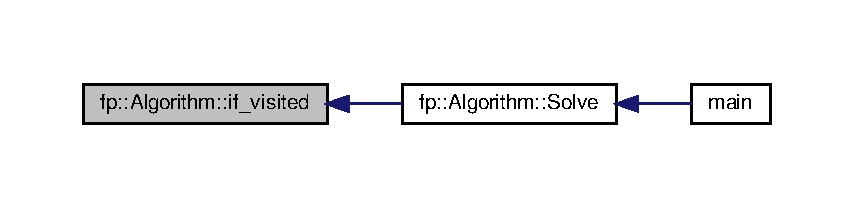
\includegraphics[width=350pt]{classfp_1_1_algorithm_aa7083be9be18b81bedf9bcc9976e97af_icgraph}
\end{center}
\end{figure}
\mbox{\Hypertarget{classfp_1_1_algorithm_a237fc28eed2899786cd06f4e5a0e7333}\label{classfp_1_1_algorithm_a237fc28eed2899786cd06f4e5a0e7333}} 
\index{fp\+::\+Algorithm@{fp\+::\+Algorithm}!is\+Goal@{is\+Goal}}
\index{is\+Goal@{is\+Goal}!fp\+::\+Algorithm@{fp\+::\+Algorithm}}
\subsubsection{\texorpdfstring{is\+Goal()}{isGoal()}}
{\footnotesize\ttfamily bool fp\+::\+Algorithm\+::is\+Goal (\begin{DoxyParamCaption}\item[{int}]{x,  }\item[{int}]{y }\end{DoxyParamCaption})}



a function to check wether we have visited nodes or not. 

a function to check wether it s goal or not


\begin{DoxyParams}{Parameters}
{\em x-\/ordinate} & \\
\hline
\end{DoxyParams}
\begin{DoxyReturn}{Returns}
y-\/coordinate 
\end{DoxyReturn}
\hypertarget{_m_a_z_e_8h_DESCRIPTION}{}\subsection{D\+E\+S\+C\+R\+I\+P\+T\+I\+ON}\label{_m_a_z_e_8h_DESCRIPTION}
A function is check x-\/y co-\/ordinates and check if we are in middle of maze it is end of game. Here is the caller graph for this function\+:
\nopagebreak
\begin{figure}[H]
\begin{center}
\leavevmode
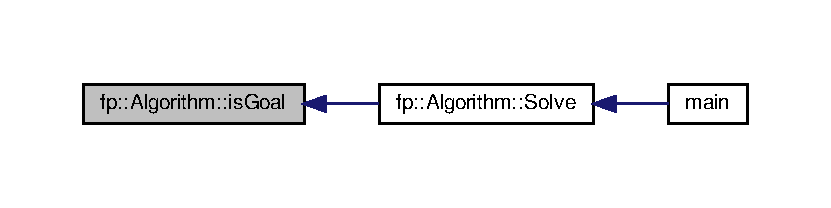
\includegraphics[width=350pt]{classfp_1_1_algorithm_a237fc28eed2899786cd06f4e5a0e7333_icgraph}
\end{center}
\end{figure}
\mbox{\Hypertarget{classfp_1_1_algorithm_a2e66300e1507ff3f71d5fbbffede52a3}\label{classfp_1_1_algorithm_a2e66300e1507ff3f71d5fbbffede52a3}} 
\index{fp\+::\+Algorithm@{fp\+::\+Algorithm}!Solve@{Solve}}
\index{Solve@{Solve}!fp\+::\+Algorithm@{fp\+::\+Algorithm}}
\subsubsection{\texorpdfstring{Solve()}{Solve()}}
{\footnotesize\ttfamily bool fp\+::\+Algorithm\+::\+Solve (\begin{DoxyParamCaption}\item[{std\+::shared\+\_\+ptr$<$ \hyperlink{classfp_1_1_land_based_robot}{fp\+::\+Land\+Based\+Robot} $>$}]{robot,  }\item[{\hyperlink{classfp_1_1_maze}{fp\+::\+Maze} \&}]{maze }\end{DoxyParamCaption})}



function is the gist of B\+FS \hyperlink{classfp_1_1_algorithm}{Algorithm}. 

heart of algorithm

\begin{DoxyReturn}{Returns}
None 
\end{DoxyReturn}

\begin{DoxyParams}{Parameters}
{\em a} & shared pointer of landbased robot class \\
\hline
{\em maze} & object \\
\hline
\end{DoxyParams}
\hypertarget{_m_a_z_e_8h_DESCRIPTION}{}\subsection{D\+E\+S\+C\+R\+I\+P\+T\+I\+ON}\label{_m_a_z_e_8h_DESCRIPTION}
This is fairly complex function but mainly we are setting the variable here and then try to push them into a vector we also set a flag which shows wether this process has ended or not. but basically a while condition shows that we will add nodes to current nodes untill we the path is found. The method we see here is basically moves robot from api file and then we check the boudries. Here is the call graph for this function\+:
\nopagebreak
\begin{figure}[H]
\begin{center}
\leavevmode
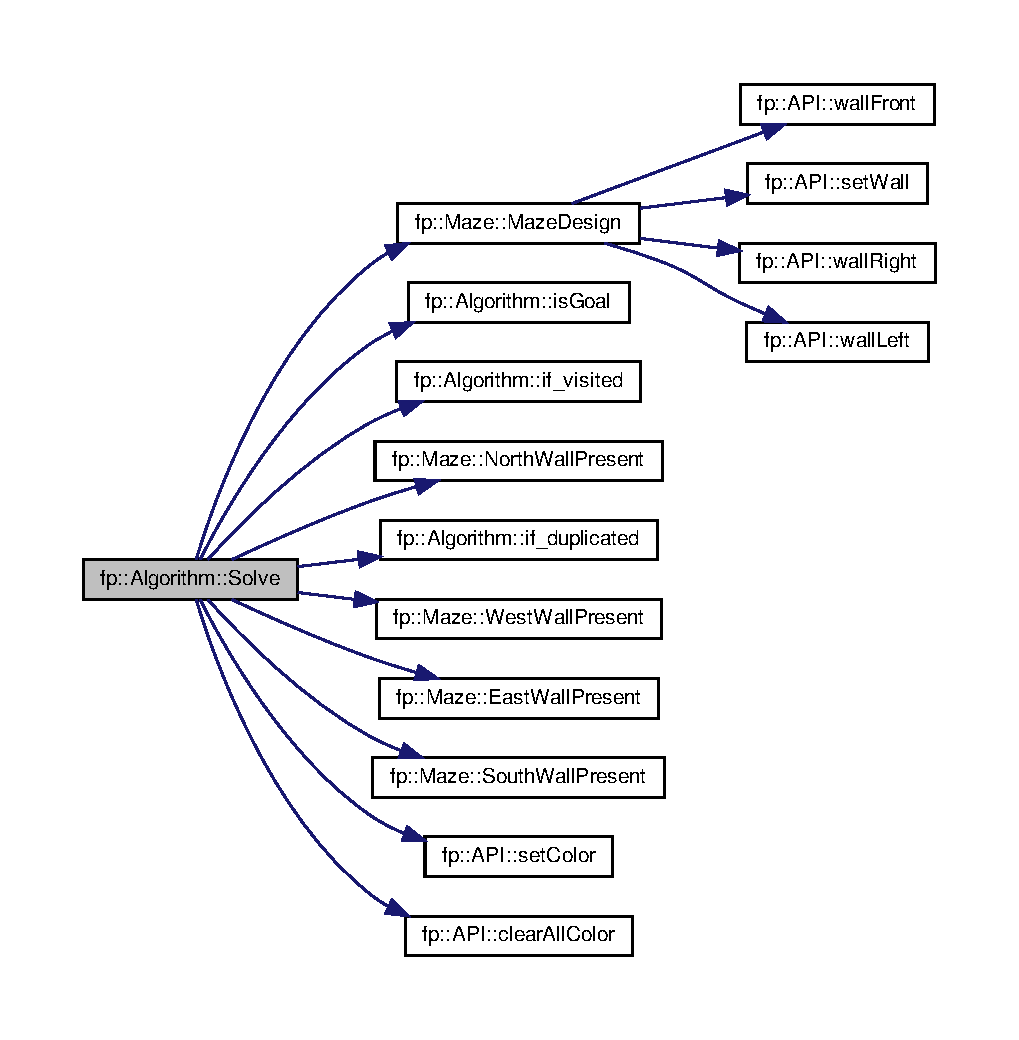
\includegraphics[width=350pt]{classfp_1_1_algorithm_a2e66300e1507ff3f71d5fbbffede52a3_cgraph}
\end{center}
\end{figure}
Here is the caller graph for this function\+:
\nopagebreak
\begin{figure}[H]
\begin{center}
\leavevmode
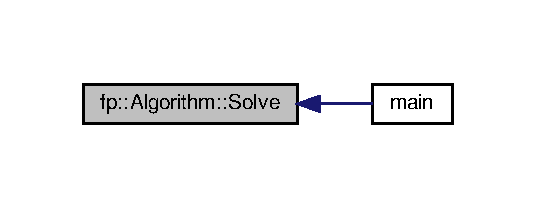
\includegraphics[width=257pt]{classfp_1_1_algorithm_a2e66300e1507ff3f71d5fbbffede52a3_icgraph}
\end{center}
\end{figure}


The documentation for this class was generated from the following files\+:\begin{DoxyCompactItemize}
\item 
src/\+Algorithm/\hyperlink{_algorithm_8h}{Algorithm.\+h}\item 
src/\+Algorithm/\hyperlink{_algorithm_8cpp}{Algorithm.\+cpp}\end{DoxyCompactItemize}

\hypertarget{classfp_1_1_a_p_i}{}\section{fp\+:\+:A\+PI Class Reference}
\label{classfp_1_1_a_p_i}\index{fp\+::\+A\+PI@{fp\+::\+A\+PI}}


{\ttfamily \#include $<$api.\+h$>$}

\subsection*{Static Public Member Functions}
\begin{DoxyCompactItemize}
\item 
static int \hyperlink{classfp_1_1_a_p_i_af8adb8d6fe6b921de4172111b32fc710}{maze\+Width} ()
\begin{DoxyCompactList}\small\item\em a function to take mazewidth from the user. \end{DoxyCompactList}\item 
static int \hyperlink{classfp_1_1_a_p_i_a7d9285544497a39f87e841fcfe49deab}{maze\+Height} ()
\begin{DoxyCompactList}\small\item\em a function to take mazeheight from the user. \end{DoxyCompactList}\item 
static bool \hyperlink{classfp_1_1_a_p_i_a52c23ca6b94cd561727e63c4a568bb86}{wall\+Front} ()
\begin{DoxyCompactList}\small\item\em a function to set in front of robot. \end{DoxyCompactList}\item 
static bool \hyperlink{classfp_1_1_a_p_i_aeaebbd3b022bc0ed768dc3112ea1db94}{wall\+Right} ()
\begin{DoxyCompactList}\small\item\em a function to wall in right hand direction. \end{DoxyCompactList}\item 
static bool \hyperlink{classfp_1_1_a_p_i_a49efec34a5521b6a7f202759f7f758d2}{wall\+Left} ()
\begin{DoxyCompactList}\small\item\em a function to wall in left hand direction. \end{DoxyCompactList}\item 
static void \hyperlink{classfp_1_1_a_p_i_a4863c0dec23d677c5eefb7c03088b29c}{move\+Forward} ()
\begin{DoxyCompactList}\small\item\em a function to move robot forward. \end{DoxyCompactList}\item 
static void \hyperlink{classfp_1_1_a_p_i_ac346f1c3ae7a39829c16681be2f25e92}{turn\+Right} ()
\begin{DoxyCompactList}\small\item\em a function to turn robot right. \end{DoxyCompactList}\item 
static void \hyperlink{classfp_1_1_a_p_i_aacf09d263f8c47e7f3eae1f348db0b91}{turn\+Left} ()
\begin{DoxyCompactList}\small\item\em a function to turn robot left \end{DoxyCompactList}\item 
static void \hyperlink{classfp_1_1_a_p_i_a5f209e53ce63ad478bb67b120b34c7dd}{set\+Wall} (int x, int y, char direction)
\begin{DoxyCompactList}\small\item\em a function to set a wall. \end{DoxyCompactList}\item 
static void \hyperlink{classfp_1_1_a_p_i_a19710a245ad8c075066046617ea3377b}{clear\+Wall} (int x, int y, char direction)
\begin{DoxyCompactList}\small\item\em a function to clear a wall. \end{DoxyCompactList}\item 
static void \hyperlink{classfp_1_1_a_p_i_a5a7c59cffb4ca483e8c1334a99a04dbb}{set\+Color} (int x, int y, char color)
\begin{DoxyCompactList}\small\item\em a function to set a color wall \end{DoxyCompactList}\item 
static void \hyperlink{classfp_1_1_a_p_i_a5ab1560f68fb54993c8b3316177040a5}{clear\+Color} (int x, int y)
\begin{DoxyCompactList}\small\item\em a function to clear a color wall \end{DoxyCompactList}\item 
static void \hyperlink{classfp_1_1_a_p_i_a68f86debe50e6e2ae0c1fde795a1cfb6}{clear\+All\+Color} ()
\begin{DoxyCompactList}\small\item\em a function to clear all color \end{DoxyCompactList}\item 
static void \hyperlink{classfp_1_1_a_p_i_a4635f5c0c48d2ab53f4436be402c5566}{set\+Text} (int x, int y, const std\+::string \&text)
\begin{DoxyCompactList}\small\item\em a function to print x-\/y with text given. \end{DoxyCompactList}\item 
static void \hyperlink{classfp_1_1_a_p_i_a0b23c3b22476d1826987b93b518010d1}{clear\+Text} (int x, int y)
\begin{DoxyCompactList}\small\item\em a function to clear text. \end{DoxyCompactList}\item 
static void \hyperlink{classfp_1_1_a_p_i_ae0b4d27428aad11e98647b88947f2c34}{clear\+All\+Text} ()
\begin{DoxyCompactList}\small\item\em print out cleatext message. \end{DoxyCompactList}\item 
static bool \hyperlink{classfp_1_1_a_p_i_a390976eee05262068b7387f1421d906a}{was\+Reset} ()
\begin{DoxyCompactList}\small\item\em print out reset message and set respose as true \end{DoxyCompactList}\item 
static void \hyperlink{classfp_1_1_a_p_i_a0c30419c7237b12bc916ce17f93a5be4}{ack\+Reset} ()
\begin{DoxyCompactList}\small\item\em print out reset message \char`\"{}ack\+Reset\char`\"{} \end{DoxyCompactList}\end{DoxyCompactItemize}


\subsection{Detailed Description}
\begin{DoxyAuthor}{Author}
Group-\/9-\/\+E\+N\+P\+M809Y 
\end{DoxyAuthor}
\begin{DoxyDate}{Date}
03/12/19 
\end{DoxyDate}


\subsection{Member Function Documentation}
\mbox{\Hypertarget{classfp_1_1_a_p_i_a0c30419c7237b12bc916ce17f93a5be4}\label{classfp_1_1_a_p_i_a0c30419c7237b12bc916ce17f93a5be4}} 
\index{fp\+::\+A\+PI@{fp\+::\+A\+PI}!ack\+Reset@{ack\+Reset}}
\index{ack\+Reset@{ack\+Reset}!fp\+::\+A\+PI@{fp\+::\+A\+PI}}
\subsubsection{\texorpdfstring{ack\+Reset()}{ackReset()}}
{\footnotesize\ttfamily void fp\+::\+A\+P\+I\+::ack\+Reset (\begin{DoxyParamCaption}{ }\end{DoxyParamCaption})\hspace{0.3cm}{\ttfamily [static]}}



print out reset message \char`\"{}ack\+Reset\char`\"{} 

a bool method to set a a string variable


\begin{DoxyParams}{Parameters}
{\em None} & -\/ void function \\
\hline
\end{DoxyParams}
\begin{DoxyReturn}{Returns}
None 
\end{DoxyReturn}
\hypertarget{_m_a_z_e_8h_DESCRIPTION}{}\subsection{D\+E\+S\+C\+R\+I\+P\+T\+I\+ON}\label{_m_a_z_e_8h_DESCRIPTION}
This is function set string variable as ack\+Reset. \mbox{\Hypertarget{classfp_1_1_a_p_i_a68f86debe50e6e2ae0c1fde795a1cfb6}\label{classfp_1_1_a_p_i_a68f86debe50e6e2ae0c1fde795a1cfb6}} 
\index{fp\+::\+A\+PI@{fp\+::\+A\+PI}!clear\+All\+Color@{clear\+All\+Color}}
\index{clear\+All\+Color@{clear\+All\+Color}!fp\+::\+A\+PI@{fp\+::\+A\+PI}}
\subsubsection{\texorpdfstring{clear\+All\+Color()}{clearAllColor()}}
{\footnotesize\ttfamily void fp\+::\+A\+P\+I\+::clear\+All\+Color (\begin{DoxyParamCaption}{ }\end{DoxyParamCaption})\hspace{0.3cm}{\ttfamily [static]}}



a function to clear all color 

a void method to print message


\begin{DoxyParams}{Parameters}
{\em None} & -\/ void function \\
\hline
\end{DoxyParams}
\begin{DoxyReturn}{Returns}
None 
\end{DoxyReturn}
\hypertarget{_m_a_z_e_8h_DESCRIPTION}{}\subsection{D\+E\+S\+C\+R\+I\+P\+T\+I\+ON}\label{_m_a_z_e_8h_DESCRIPTION}
This is function print clearall. Here is the caller graph for this function\+:
\nopagebreak
\begin{figure}[H]
\begin{center}
\leavevmode
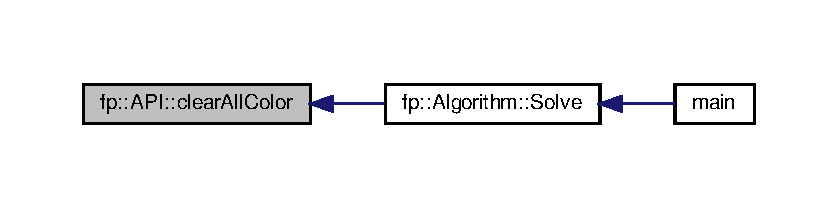
\includegraphics[width=350pt]{classfp_1_1_a_p_i_a68f86debe50e6e2ae0c1fde795a1cfb6_icgraph}
\end{center}
\end{figure}
\mbox{\Hypertarget{classfp_1_1_a_p_i_ae0b4d27428aad11e98647b88947f2c34}\label{classfp_1_1_a_p_i_ae0b4d27428aad11e98647b88947f2c34}} 
\index{fp\+::\+A\+PI@{fp\+::\+A\+PI}!clear\+All\+Text@{clear\+All\+Text}}
\index{clear\+All\+Text@{clear\+All\+Text}!fp\+::\+A\+PI@{fp\+::\+A\+PI}}
\subsubsection{\texorpdfstring{clear\+All\+Text()}{clearAllText()}}
{\footnotesize\ttfamily void fp\+::\+A\+P\+I\+::clear\+All\+Text (\begin{DoxyParamCaption}{ }\end{DoxyParamCaption})\hspace{0.3cm}{\ttfamily [static]}}



print out cleatext message. 

a void method to print meassage


\begin{DoxyParams}{Parameters}
{\em None} & -\/ void function \\
\hline
\end{DoxyParams}
\begin{DoxyReturn}{Returns}
None 
\end{DoxyReturn}
\hypertarget{_m_a_z_e_8h_DESCRIPTION}{}\subsection{D\+E\+S\+C\+R\+I\+P\+T\+I\+ON}\label{_m_a_z_e_8h_DESCRIPTION}
This is function prints out message to user. \mbox{\Hypertarget{classfp_1_1_a_p_i_a5ab1560f68fb54993c8b3316177040a5}\label{classfp_1_1_a_p_i_a5ab1560f68fb54993c8b3316177040a5}} 
\index{fp\+::\+A\+PI@{fp\+::\+A\+PI}!clear\+Color@{clear\+Color}}
\index{clear\+Color@{clear\+Color}!fp\+::\+A\+PI@{fp\+::\+A\+PI}}
\subsubsection{\texorpdfstring{clear\+Color()}{clearColor()}}
{\footnotesize\ttfamily void fp\+::\+A\+P\+I\+::clear\+Color (\begin{DoxyParamCaption}\item[{int}]{x,  }\item[{int}]{y }\end{DoxyParamCaption})\hspace{0.3cm}{\ttfamily [static]}}



a function to clear a color wall 

a void method to clear a color


\begin{DoxyParams}{Parameters}
{\em x} & co-\/ordinate \\
\hline
{\em y} & co-\/ordinate \\
\hline
\end{DoxyParams}
\begin{DoxyReturn}{Returns}
None 
\end{DoxyReturn}
\hypertarget{_m_a_z_e_8h_DESCRIPTION}{}\subsection{D\+E\+S\+C\+R\+I\+P\+T\+I\+ON}\label{_m_a_z_e_8h_DESCRIPTION}
This is function used to clear a color using given x and y parameters. \mbox{\Hypertarget{classfp_1_1_a_p_i_a0b23c3b22476d1826987b93b518010d1}\label{classfp_1_1_a_p_i_a0b23c3b22476d1826987b93b518010d1}} 
\index{fp\+::\+A\+PI@{fp\+::\+A\+PI}!clear\+Text@{clear\+Text}}
\index{clear\+Text@{clear\+Text}!fp\+::\+A\+PI@{fp\+::\+A\+PI}}
\subsubsection{\texorpdfstring{clear\+Text()}{clearText()}}
{\footnotesize\ttfamily void fp\+::\+A\+P\+I\+::clear\+Text (\begin{DoxyParamCaption}\item[{int}]{x,  }\item[{int}]{y }\end{DoxyParamCaption})\hspace{0.3cm}{\ttfamily [static]}}



a function to clear text. 

a void method to clear a color


\begin{DoxyParams}{Parameters}
{\em x} & co-\/ordinate \\
\hline
{\em y} & co-\/ordinate \\
\hline
\end{DoxyParams}
\begin{DoxyReturn}{Returns}
None 
\end{DoxyReturn}
\hypertarget{_m_a_z_e_8h_DESCRIPTION}{}\subsection{D\+E\+S\+C\+R\+I\+P\+T\+I\+ON}\label{_m_a_z_e_8h_DESCRIPTION}
This is function takes x-\/y and clear out text at that co-\/ordinate. \mbox{\Hypertarget{classfp_1_1_a_p_i_a19710a245ad8c075066046617ea3377b}\label{classfp_1_1_a_p_i_a19710a245ad8c075066046617ea3377b}} 
\index{fp\+::\+A\+PI@{fp\+::\+A\+PI}!clear\+Wall@{clear\+Wall}}
\index{clear\+Wall@{clear\+Wall}!fp\+::\+A\+PI@{fp\+::\+A\+PI}}
\subsubsection{\texorpdfstring{clear\+Wall()}{clearWall()}}
{\footnotesize\ttfamily void fp\+::\+A\+P\+I\+::clear\+Wall (\begin{DoxyParamCaption}\item[{int}]{x,  }\item[{int}]{y,  }\item[{char}]{direction }\end{DoxyParamCaption})\hspace{0.3cm}{\ttfamily [static]}}



a function to clear a wall. 

a void method to clear a wall


\begin{DoxyParams}{Parameters}
{\em x} & co-\/ordinate \\
\hline
{\em y} & co-\/ordinate \\
\hline
{\em char} & for direction \\
\hline
\end{DoxyParams}
\begin{DoxyReturn}{Returns}
None 
\end{DoxyReturn}
\hypertarget{_m_a_z_e_8h_DESCRIPTION}{}\subsection{D\+E\+S\+C\+R\+I\+P\+T\+I\+ON}\label{_m_a_z_e_8h_DESCRIPTION}
This is function clear a wall in given direction with x and y taken integers. \mbox{\Hypertarget{classfp_1_1_a_p_i_a7d9285544497a39f87e841fcfe49deab}\label{classfp_1_1_a_p_i_a7d9285544497a39f87e841fcfe49deab}} 
\index{fp\+::\+A\+PI@{fp\+::\+A\+PI}!maze\+Height@{maze\+Height}}
\index{maze\+Height@{maze\+Height}!fp\+::\+A\+PI@{fp\+::\+A\+PI}}
\subsubsection{\texorpdfstring{maze\+Height()}{mazeHeight()}}
{\footnotesize\ttfamily int fp\+::\+A\+P\+I\+::maze\+Height (\begin{DoxyParamCaption}{ }\end{DoxyParamCaption})\hspace{0.3cm}{\ttfamily [static]}}



a function to take mazeheight from the user. 

maze hieght that can not be changed and static type


\begin{DoxyParams}{Parameters}
{\em None-\/} & Void function \\
\hline
\end{DoxyParams}
\begin{DoxyReturn}{Returns}
integer 
\end{DoxyReturn}
\hypertarget{_m_a_z_e_8h_DESCRIPTION}{}\subsection{D\+E\+S\+C\+R\+I\+P\+T\+I\+ON}\label{_m_a_z_e_8h_DESCRIPTION}
A function that takes maze-\/hieght using cin and then return as a string But main use of this take response and set mazeheight variable. \mbox{\Hypertarget{classfp_1_1_a_p_i_af8adb8d6fe6b921de4172111b32fc710}\label{classfp_1_1_a_p_i_af8adb8d6fe6b921de4172111b32fc710}} 
\index{fp\+::\+A\+PI@{fp\+::\+A\+PI}!maze\+Width@{maze\+Width}}
\index{maze\+Width@{maze\+Width}!fp\+::\+A\+PI@{fp\+::\+A\+PI}}
\subsubsection{\texorpdfstring{maze\+Width()}{mazeWidth()}}
{\footnotesize\ttfamily int fp\+::\+A\+P\+I\+::maze\+Width (\begin{DoxyParamCaption}{ }\end{DoxyParamCaption})\hspace{0.3cm}{\ttfamily [static]}}



a function to take mazewidth from the user. 

maze width that can not be changed and static type


\begin{DoxyParams}{Parameters}
{\em None-\/} & Void function \\
\hline
\end{DoxyParams}
\hypertarget{_m_a_z_e_8h_DESCRIPTION}{}\subsection{D\+E\+S\+C\+R\+I\+P\+T\+I\+ON}\label{_m_a_z_e_8h_DESCRIPTION}
A function that takes mazewidth using cin and then return as a string But main use of this take response and set mazewidth variable. \mbox{\Hypertarget{classfp_1_1_a_p_i_a4863c0dec23d677c5eefb7c03088b29c}\label{classfp_1_1_a_p_i_a4863c0dec23d677c5eefb7c03088b29c}} 
\index{fp\+::\+A\+PI@{fp\+::\+A\+PI}!move\+Forward@{move\+Forward}}
\index{move\+Forward@{move\+Forward}!fp\+::\+A\+PI@{fp\+::\+A\+PI}}
\subsubsection{\texorpdfstring{move\+Forward()}{moveForward()}}
{\footnotesize\ttfamily void fp\+::\+A\+P\+I\+::move\+Forward (\begin{DoxyParamCaption}{ }\end{DoxyParamCaption})\hspace{0.3cm}{\ttfamily [static]}}



a function to move robot forward. 

a void method to move robot forward


\begin{DoxyParams}{Parameters}
{\em None} & -\/ void function \\
\hline
\end{DoxyParams}
\begin{DoxyReturn}{Returns}
None 
\end{DoxyReturn}
\hypertarget{_m_a_z_e_8h_DESCRIPTION}{}\subsection{D\+E\+S\+C\+R\+I\+P\+T\+I\+ON}\label{_m_a_z_e_8h_DESCRIPTION}
This is robot family function and used to move forward. This gives flexibility to move robot and different from wall family function. Here is the caller graph for this function\+:
\nopagebreak
\begin{figure}[H]
\begin{center}
\leavevmode
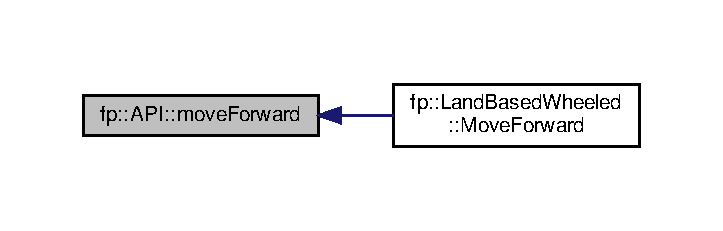
\includegraphics[width=347pt]{classfp_1_1_a_p_i_a4863c0dec23d677c5eefb7c03088b29c_icgraph}
\end{center}
\end{figure}
\mbox{\Hypertarget{classfp_1_1_a_p_i_a5a7c59cffb4ca483e8c1334a99a04dbb}\label{classfp_1_1_a_p_i_a5a7c59cffb4ca483e8c1334a99a04dbb}} 
\index{fp\+::\+A\+PI@{fp\+::\+A\+PI}!set\+Color@{set\+Color}}
\index{set\+Color@{set\+Color}!fp\+::\+A\+PI@{fp\+::\+A\+PI}}
\subsubsection{\texorpdfstring{set\+Color()}{setColor()}}
{\footnotesize\ttfamily void fp\+::\+A\+P\+I\+::set\+Color (\begin{DoxyParamCaption}\item[{int}]{x,  }\item[{int}]{y,  }\item[{char}]{color }\end{DoxyParamCaption})\hspace{0.3cm}{\ttfamily [static]}}



a function to set a color wall 

a void method to set a color


\begin{DoxyParams}{Parameters}
{\em x} & co-\/ordinate \\
\hline
{\em y} & co-\/ordinate \\
\hline
{\em char} & for color \\
\hline
\end{DoxyParams}
\begin{DoxyReturn}{Returns}
None 
\end{DoxyReturn}
\hypertarget{_m_a_z_e_8h_DESCRIPTION}{}\subsection{D\+E\+S\+C\+R\+I\+P\+T\+I\+ON}\label{_m_a_z_e_8h_DESCRIPTION}
This is function used to set a color taken as \char`\"{}color parameter\char`\"{} and set using x-\/y coordinates. Here is the caller graph for this function\+:
\nopagebreak
\begin{figure}[H]
\begin{center}
\leavevmode
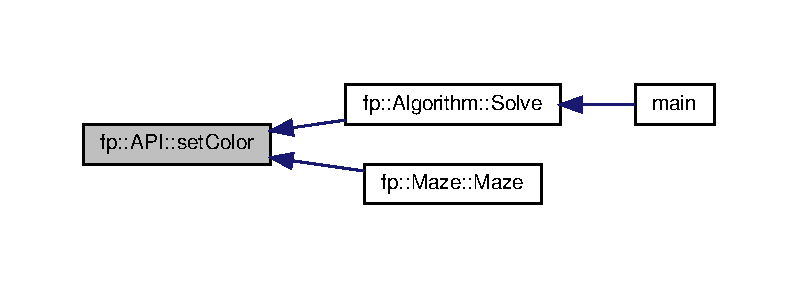
\includegraphics[width=350pt]{classfp_1_1_a_p_i_a5a7c59cffb4ca483e8c1334a99a04dbb_icgraph}
\end{center}
\end{figure}
\mbox{\Hypertarget{classfp_1_1_a_p_i_a4635f5c0c48d2ab53f4436be402c5566}\label{classfp_1_1_a_p_i_a4635f5c0c48d2ab53f4436be402c5566}} 
\index{fp\+::\+A\+PI@{fp\+::\+A\+PI}!set\+Text@{set\+Text}}
\index{set\+Text@{set\+Text}!fp\+::\+A\+PI@{fp\+::\+A\+PI}}
\subsubsection{\texorpdfstring{set\+Text()}{setText()}}
{\footnotesize\ttfamily void fp\+::\+A\+P\+I\+::set\+Text (\begin{DoxyParamCaption}\item[{int}]{x,  }\item[{int}]{y,  }\item[{const std\+::string \&}]{text }\end{DoxyParamCaption})\hspace{0.3cm}{\ttfamily [static]}}



a function to print x-\/y with text given. 

a void method to set a text


\begin{DoxyParams}{Parameters}
{\em x} & co-\/ordinate \\
\hline
{\em y} & co-\/ordinate \\
\hline
{\em string} & as text \\
\hline
\end{DoxyParams}
\begin{DoxyReturn}{Returns}
None 
\end{DoxyReturn}
\hypertarget{_m_a_z_e_8h_DESCRIPTION}{}\subsection{D\+E\+S\+C\+R\+I\+P\+T\+I\+ON}\label{_m_a_z_e_8h_DESCRIPTION}
This is function takes x-\/y and print out text at that co-\/ordinate. Here is the caller graph for this function\+:
\nopagebreak
\begin{figure}[H]
\begin{center}
\leavevmode
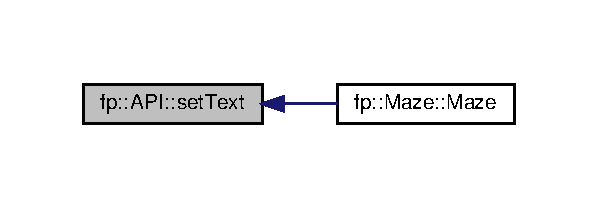
\includegraphics[width=287pt]{classfp_1_1_a_p_i_a4635f5c0c48d2ab53f4436be402c5566_icgraph}
\end{center}
\end{figure}
\mbox{\Hypertarget{classfp_1_1_a_p_i_a5f209e53ce63ad478bb67b120b34c7dd}\label{classfp_1_1_a_p_i_a5f209e53ce63ad478bb67b120b34c7dd}} 
\index{fp\+::\+A\+PI@{fp\+::\+A\+PI}!set\+Wall@{set\+Wall}}
\index{set\+Wall@{set\+Wall}!fp\+::\+A\+PI@{fp\+::\+A\+PI}}
\subsubsection{\texorpdfstring{set\+Wall()}{setWall()}}
{\footnotesize\ttfamily void fp\+::\+A\+P\+I\+::set\+Wall (\begin{DoxyParamCaption}\item[{int}]{x,  }\item[{int}]{y,  }\item[{char}]{direction }\end{DoxyParamCaption})\hspace{0.3cm}{\ttfamily [static]}}



a function to set a wall. 

a void method to set a wall


\begin{DoxyParams}{Parameters}
{\em x} & co-\/ordinate \\
\hline
{\em y} & co-\/ordinate \\
\hline
{\em char} & for direction \\
\hline
\end{DoxyParams}
\begin{DoxyReturn}{Returns}
None 
\end{DoxyReturn}
\hypertarget{_m_a_z_e_8h_DESCRIPTION}{}\subsection{D\+E\+S\+C\+R\+I\+P\+T\+I\+ON}\label{_m_a_z_e_8h_DESCRIPTION}
This is function set a wall in given direction with x and y taken integers. Here is the caller graph for this function\+:
\nopagebreak
\begin{figure}[H]
\begin{center}
\leavevmode
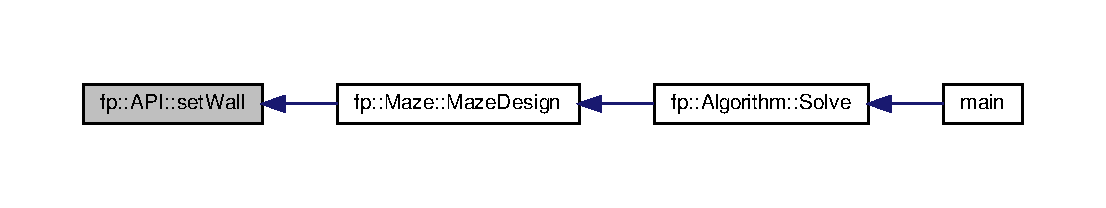
\includegraphics[width=350pt]{classfp_1_1_a_p_i_a5f209e53ce63ad478bb67b120b34c7dd_icgraph}
\end{center}
\end{figure}
\mbox{\Hypertarget{classfp_1_1_a_p_i_aacf09d263f8c47e7f3eae1f348db0b91}\label{classfp_1_1_a_p_i_aacf09d263f8c47e7f3eae1f348db0b91}} 
\index{fp\+::\+A\+PI@{fp\+::\+A\+PI}!turn\+Left@{turn\+Left}}
\index{turn\+Left@{turn\+Left}!fp\+::\+A\+PI@{fp\+::\+A\+PI}}
\subsubsection{\texorpdfstring{turn\+Left()}{turnLeft()}}
{\footnotesize\ttfamily void fp\+::\+A\+P\+I\+::turn\+Left (\begin{DoxyParamCaption}{ }\end{DoxyParamCaption})\hspace{0.3cm}{\ttfamily [static]}}



a function to turn robot left 

a void method to move turn robot left


\begin{DoxyParams}{Parameters}
{\em None} & -\/ void function \\
\hline
\end{DoxyParams}
\begin{DoxyReturn}{Returns}
None 
\end{DoxyReturn}
\hypertarget{_m_a_z_e_8h_DESCRIPTION}{}\subsection{D\+E\+S\+C\+R\+I\+P\+T\+I\+ON}\label{_m_a_z_e_8h_DESCRIPTION}
This is robot family function and used to turnleft. This gives flexibility to move robot and different from wall family function. Here is the caller graph for this function\+:
\nopagebreak
\begin{figure}[H]
\begin{center}
\leavevmode
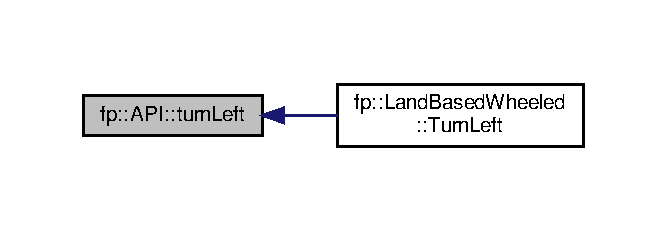
\includegraphics[width=320pt]{classfp_1_1_a_p_i_aacf09d263f8c47e7f3eae1f348db0b91_icgraph}
\end{center}
\end{figure}
\mbox{\Hypertarget{classfp_1_1_a_p_i_ac346f1c3ae7a39829c16681be2f25e92}\label{classfp_1_1_a_p_i_ac346f1c3ae7a39829c16681be2f25e92}} 
\index{fp\+::\+A\+PI@{fp\+::\+A\+PI}!turn\+Right@{turn\+Right}}
\index{turn\+Right@{turn\+Right}!fp\+::\+A\+PI@{fp\+::\+A\+PI}}
\subsubsection{\texorpdfstring{turn\+Right()}{turnRight()}}
{\footnotesize\ttfamily void fp\+::\+A\+P\+I\+::turn\+Right (\begin{DoxyParamCaption}{ }\end{DoxyParamCaption})\hspace{0.3cm}{\ttfamily [static]}}



a function to turn robot right. 

a void method to move turn robot right


\begin{DoxyParams}{Parameters}
{\em None} & -\/ void function \\
\hline
\end{DoxyParams}
\begin{DoxyReturn}{Returns}
None 
\end{DoxyReturn}
\hypertarget{_m_a_z_e_8h_DESCRIPTION}{}\subsection{D\+E\+S\+C\+R\+I\+P\+T\+I\+ON}\label{_m_a_z_e_8h_DESCRIPTION}
This is robot family function and used to turn right. This gives flexibility to move robot and different from wall family function. Here is the caller graph for this function\+:
\nopagebreak
\begin{figure}[H]
\begin{center}
\leavevmode
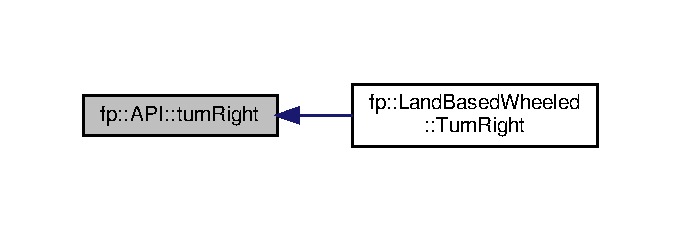
\includegraphics[width=327pt]{classfp_1_1_a_p_i_ac346f1c3ae7a39829c16681be2f25e92_icgraph}
\end{center}
\end{figure}
\mbox{\Hypertarget{classfp_1_1_a_p_i_a52c23ca6b94cd561727e63c4a568bb86}\label{classfp_1_1_a_p_i_a52c23ca6b94cd561727e63c4a568bb86}} 
\index{fp\+::\+A\+PI@{fp\+::\+A\+PI}!wall\+Front@{wall\+Front}}
\index{wall\+Front@{wall\+Front}!fp\+::\+A\+PI@{fp\+::\+A\+PI}}
\subsubsection{\texorpdfstring{wall\+Front()}{wallFront()}}
{\footnotesize\ttfamily bool fp\+::\+A\+P\+I\+::wall\+Front (\begin{DoxyParamCaption}{ }\end{DoxyParamCaption})\hspace{0.3cm}{\ttfamily [static]}}



a function to set in front of robot. 

a boolean to check wether ther is wall in front or not.


\begin{DoxyParams}{Parameters}
{\em None} & -\/ void function \\
\hline
\end{DoxyParams}
\begin{DoxyReturn}{Returns}
True or False 
\end{DoxyReturn}
\hypertarget{_m_a_z_e_8h_DESCRIPTION}{}\subsection{D\+E\+S\+C\+R\+I\+P\+T\+I\+ON}\label{_m_a_z_e_8h_DESCRIPTION}
A function is taking a respose from the robot and then after execution set a wall in front of it. We wanted to set wall as robot moves and discovers the maze so this is one of this important function to set a wall. Here is the caller graph for this function\+:
\nopagebreak
\begin{figure}[H]
\begin{center}
\leavevmode
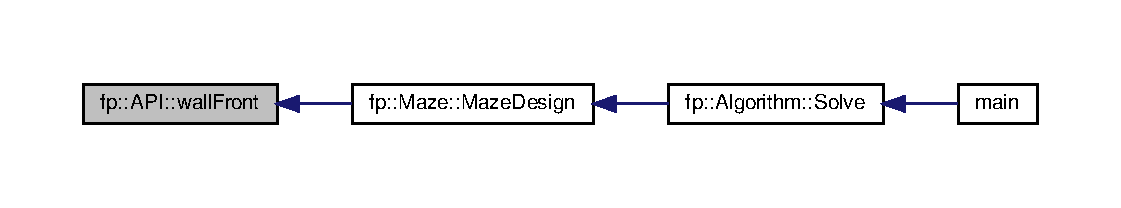
\includegraphics[width=350pt]{classfp_1_1_a_p_i_a52c23ca6b94cd561727e63c4a568bb86_icgraph}
\end{center}
\end{figure}
\mbox{\Hypertarget{classfp_1_1_a_p_i_a49efec34a5521b6a7f202759f7f758d2}\label{classfp_1_1_a_p_i_a49efec34a5521b6a7f202759f7f758d2}} 
\index{fp\+::\+A\+PI@{fp\+::\+A\+PI}!wall\+Left@{wall\+Left}}
\index{wall\+Left@{wall\+Left}!fp\+::\+A\+PI@{fp\+::\+A\+PI}}
\subsubsection{\texorpdfstring{wall\+Left()}{wallLeft()}}
{\footnotesize\ttfamily bool fp\+::\+A\+P\+I\+::wall\+Left (\begin{DoxyParamCaption}{ }\end{DoxyParamCaption})\hspace{0.3cm}{\ttfamily [static]}}



a function to wall in left hand direction. 

a boolean to check wether ther is wall in left or not.


\begin{DoxyParams}{Parameters}
{\em None} & -\/ void function \\
\hline
\end{DoxyParams}
\begin{DoxyReturn}{Returns}
True or False 
\end{DoxyReturn}
\hypertarget{_m_a_z_e_8h_DESCRIPTION}{}\subsection{D\+E\+S\+C\+R\+I\+P\+T\+I\+ON}\label{_m_a_z_e_8h_DESCRIPTION}
A function is taking a respose from the robot and then after execution set a wall in left side of robot. We wanted to set wall as robot moves and discovers the maze so this is one of this important function to set a wall. Here is the caller graph for this function\+:
\nopagebreak
\begin{figure}[H]
\begin{center}
\leavevmode
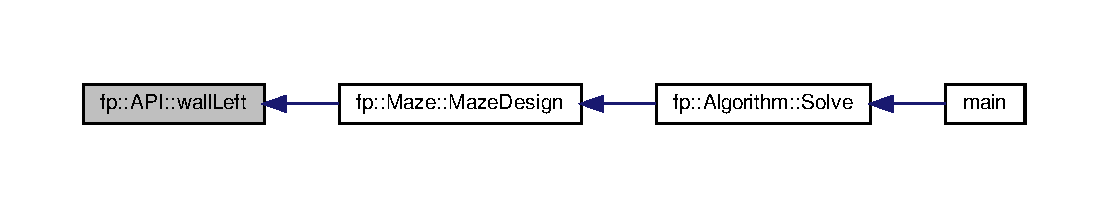
\includegraphics[width=350pt]{classfp_1_1_a_p_i_a49efec34a5521b6a7f202759f7f758d2_icgraph}
\end{center}
\end{figure}
\mbox{\Hypertarget{classfp_1_1_a_p_i_aeaebbd3b022bc0ed768dc3112ea1db94}\label{classfp_1_1_a_p_i_aeaebbd3b022bc0ed768dc3112ea1db94}} 
\index{fp\+::\+A\+PI@{fp\+::\+A\+PI}!wall\+Right@{wall\+Right}}
\index{wall\+Right@{wall\+Right}!fp\+::\+A\+PI@{fp\+::\+A\+PI}}
\subsubsection{\texorpdfstring{wall\+Right()}{wallRight()}}
{\footnotesize\ttfamily bool fp\+::\+A\+P\+I\+::wall\+Right (\begin{DoxyParamCaption}{ }\end{DoxyParamCaption})\hspace{0.3cm}{\ttfamily [static]}}



a function to wall in right hand direction. 

a boolean to check wether ther is wall in right of the robot


\begin{DoxyParams}{Parameters}
{\em None} & -\/ void function \\
\hline
\end{DoxyParams}
\begin{DoxyReturn}{Returns}
True or False 
\end{DoxyReturn}
\hypertarget{_m_a_z_e_8h_DESCRIPTION}{}\subsection{D\+E\+S\+C\+R\+I\+P\+T\+I\+ON}\label{_m_a_z_e_8h_DESCRIPTION}
A function is taking a respose from the robot and then after execution set a wall in right side of robot. We wanted to set wall as robot moves and discovers the maze so this is one of this important function to set a wall. Here is the caller graph for this function\+:
\nopagebreak
\begin{figure}[H]
\begin{center}
\leavevmode
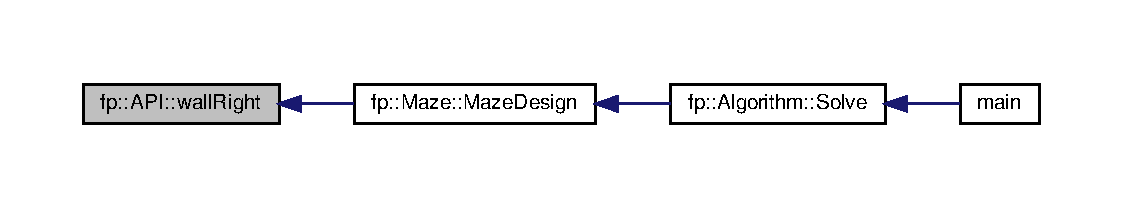
\includegraphics[width=350pt]{classfp_1_1_a_p_i_aeaebbd3b022bc0ed768dc3112ea1db94_icgraph}
\end{center}
\end{figure}
\mbox{\Hypertarget{classfp_1_1_a_p_i_a390976eee05262068b7387f1421d906a}\label{classfp_1_1_a_p_i_a390976eee05262068b7387f1421d906a}} 
\index{fp\+::\+A\+PI@{fp\+::\+A\+PI}!was\+Reset@{was\+Reset}}
\index{was\+Reset@{was\+Reset}!fp\+::\+A\+PI@{fp\+::\+A\+PI}}
\subsubsection{\texorpdfstring{was\+Reset()}{wasReset()}}
{\footnotesize\ttfamily bool fp\+::\+A\+P\+I\+::was\+Reset (\begin{DoxyParamCaption}{ }\end{DoxyParamCaption})\hspace{0.3cm}{\ttfamily [static]}}



print out reset message and set respose as true 

a bool method to set a a string variable


\begin{DoxyParams}{Parameters}
{\em None} & -\/ void function \\
\hline
\end{DoxyParams}
\begin{DoxyReturn}{Returns}
True/\+False 
\end{DoxyReturn}
\hypertarget{_m_a_z_e_8h_DESCRIPTION}{}\subsection{D\+E\+S\+C\+R\+I\+P\+T\+I\+ON}\label{_m_a_z_e_8h_DESCRIPTION}
This is function take a respose using cin and set it to true. 

The documentation for this class was generated from the following files\+:\begin{DoxyCompactItemize}
\item 
src/\+A\+P\+I/\hyperlink{api_8h}{api.\+h}\item 
src/\+A\+P\+I/\hyperlink{api_8cpp}{api.\+cpp}\end{DoxyCompactItemize}

\hypertarget{classfp_1_1_land_based_robot}{}\section{fp\+:\+:Land\+Based\+Robot Class Reference}
\label{classfp_1_1_land_based_robot}\index{fp\+::\+Land\+Based\+Robot@{fp\+::\+Land\+Based\+Robot}}


{\ttfamily \#include $<$Land\+Based\+Robot.\+h$>$}



Inheritance diagram for fp\+:\+:Land\+Based\+Robot\+:
\nopagebreak
\begin{figure}[H]
\begin{center}
\leavevmode
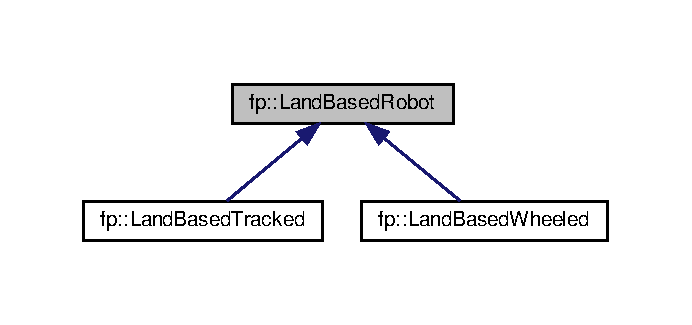
\includegraphics[width=332pt]{classfp_1_1_land_based_robot__inherit__graph}
\end{center}
\end{figure}
\subsection*{Public Member Functions}
\begin{DoxyCompactItemize}
\item 
\hyperlink{classfp_1_1_land_based_robot_a3aabd7151068be36ba93ff5813223e0c}{Land\+Based\+Robot} (std\+::string name, int x, int y)
\item 
\hyperlink{classfp_1_1_land_based_robot_a3e16cc74a11f831186978ef27eca7b99}{Land\+Based\+Robot} ()
\item 
\hyperlink{classfp_1_1_land_based_robot_ad62091990dd9e40e9c68f7c52914be93}{$\sim$\+Land\+Based\+Robot} ()
\item 
virtual void \hyperlink{classfp_1_1_land_based_robot_a5df828c5d6c1f7fb4c7b68f53d9c6080}{Move\+Forward} ()=0
\item 
virtual void \hyperlink{classfp_1_1_land_based_robot_a359e1012e9093475b7a1b0d38e41a118}{Turn\+Left} (int x, int y)=0
\begin{DoxyCompactList}\small\item\em This will just ouput that appropriate function are called or not. \end{DoxyCompactList}\item 
virtual void \hyperlink{classfp_1_1_land_based_robot_a7360e4084bc5254f72ab0d3612644907}{Turn\+Right} (int x, int y)=0
\begin{DoxyCompactList}\small\item\em This will just ouput that appropriate function are called or not. \end{DoxyCompactList}\item 
virtual int \hyperlink{classfp_1_1_land_based_robot_a3624c5d041de0987c0103c6b01fa9bc6}{get\+\_\+x} ()=0
\begin{DoxyCompactList}\small\item\em This will just ouput that appropriate function are called or not. \end{DoxyCompactList}\item 
virtual int \hyperlink{classfp_1_1_land_based_robot_ae742797bee07ac5b92bfe934cbfed6e9}{get\+\_\+y} ()=0
\begin{DoxyCompactList}\small\item\em This will just ouput that appropriate function are called or not. \end{DoxyCompactList}\item 
virtual char \hyperlink{classfp_1_1_land_based_robot_a50841b6e40d4e92832770d26b427fea2}{Get\+Direction} ()=0
\begin{DoxyCompactList}\small\item\em This will get direction of robot. \end{DoxyCompactList}\item 
virtual double \hyperlink{classfp_1_1_land_based_robot_a68844e9c442d1b293945144dc6c6608c}{get\+\_\+speed} ()=0
\begin{DoxyCompactList}\small\item\em This function gets the spped of landbased robot. \end{DoxyCompactList}\end{DoxyCompactItemize}
\subsection*{Protected Attributes}
\begin{DoxyCompactItemize}
\item 
std\+::string \hyperlink{classfp_1_1_land_based_robot_ac79ca2c52e99bc96534bb7a57dcb9030}{name\+\_\+}
\item 
int \hyperlink{classfp_1_1_land_based_robot_a55c2b5865fd60fb0158a135031f8b271}{x\+\_\+}
\item 
int \hyperlink{classfp_1_1_land_based_robot_a130cfd6ad383116076dc891ee3a52671}{y\+\_\+}
\item 
double \hyperlink{classfp_1_1_land_based_robot_ae969157e5f910ed0a85198dc7f6c3cef}{speed\+\_\+}
\item 
double \hyperlink{classfp_1_1_land_based_robot_aae605323e9ce63f29dcded204421b1fc}{width\+\_\+}
\item 
double \hyperlink{classfp_1_1_land_based_robot_a9475d5886f329c92e68f0d86b4da58c0}{length\+\_\+}
\item 
double \hyperlink{classfp_1_1_land_based_robot_a34238a27d9055c416a3e6cfedc8ed248}{height\+\_\+}
\item 
double \hyperlink{classfp_1_1_land_based_robot_a542d90c7c62899e3c3cf28791bbb6c8e}{capacity\+\_\+}
\item 
char \hyperlink{classfp_1_1_land_based_robot_adc8e6123fa8ffe86576e46000b0ae779}{direction\+\_\+}
\end{DoxyCompactItemize}


\subsection{Constructor \& Destructor Documentation}
\mbox{\Hypertarget{classfp_1_1_land_based_robot_a3aabd7151068be36ba93ff5813223e0c}\label{classfp_1_1_land_based_robot_a3aabd7151068be36ba93ff5813223e0c}} 
\index{fp\+::\+Land\+Based\+Robot@{fp\+::\+Land\+Based\+Robot}!Land\+Based\+Robot@{Land\+Based\+Robot}}
\index{Land\+Based\+Robot@{Land\+Based\+Robot}!fp\+::\+Land\+Based\+Robot@{fp\+::\+Land\+Based\+Robot}}
\subsubsection{\texorpdfstring{Land\+Based\+Robot()}{LandBasedRobot()}\hspace{0.1cm}{\footnotesize\ttfamily [1/2]}}
{\footnotesize\ttfamily fp\+::\+Land\+Based\+Robot\+::\+Land\+Based\+Robot (\begin{DoxyParamCaption}\item[{std\+::string}]{name,  }\item[{int}]{x,  }\item[{int}]{y }\end{DoxyParamCaption})}

A constructor. A constructor which takes name, x, and y as arguments and sets these parameters. \mbox{\Hypertarget{classfp_1_1_land_based_robot_a3e16cc74a11f831186978ef27eca7b99}\label{classfp_1_1_land_based_robot_a3e16cc74a11f831186978ef27eca7b99}} 
\index{fp\+::\+Land\+Based\+Robot@{fp\+::\+Land\+Based\+Robot}!Land\+Based\+Robot@{Land\+Based\+Robot}}
\index{Land\+Based\+Robot@{Land\+Based\+Robot}!fp\+::\+Land\+Based\+Robot@{fp\+::\+Land\+Based\+Robot}}
\subsubsection{\texorpdfstring{Land\+Based\+Robot()}{LandBasedRobot()}\hspace{0.1cm}{\footnotesize\ttfamily [2/2]}}
{\footnotesize\ttfamily fp\+::\+Land\+Based\+Robot\+::\+Land\+Based\+Robot (\begin{DoxyParamCaption}{ }\end{DoxyParamCaption})}

A constructor. A constructor which takes no arguments and initializes name to none and x \& y to 0. \mbox{\Hypertarget{classfp_1_1_land_based_robot_ad62091990dd9e40e9c68f7c52914be93}\label{classfp_1_1_land_based_robot_ad62091990dd9e40e9c68f7c52914be93}} 
\index{fp\+::\+Land\+Based\+Robot@{fp\+::\+Land\+Based\+Robot}!````~Land\+Based\+Robot@{$\sim$\+Land\+Based\+Robot}}
\index{````~Land\+Based\+Robot@{$\sim$\+Land\+Based\+Robot}!fp\+::\+Land\+Based\+Robot@{fp\+::\+Land\+Based\+Robot}}
\subsubsection{\texorpdfstring{$\sim$\+Land\+Based\+Robot()}{~LandBasedRobot()}}
{\footnotesize\ttfamily fp\+::\+Land\+Based\+Robot\+::$\sim$\+Land\+Based\+Robot (\begin{DoxyParamCaption}{ }\end{DoxyParamCaption})}

A destructor. This will destroy the object \hyperlink{classfp_1_1_land_based_wheeled}{Land\+Based\+Wheeled} after use 

\subsection{Member Function Documentation}
\mbox{\Hypertarget{classfp_1_1_land_based_robot_a68844e9c442d1b293945144dc6c6608c}\label{classfp_1_1_land_based_robot_a68844e9c442d1b293945144dc6c6608c}} 
\index{fp\+::\+Land\+Based\+Robot@{fp\+::\+Land\+Based\+Robot}!get\+\_\+speed@{get\+\_\+speed}}
\index{get\+\_\+speed@{get\+\_\+speed}!fp\+::\+Land\+Based\+Robot@{fp\+::\+Land\+Based\+Robot}}
\subsubsection{\texorpdfstring{get\+\_\+speed()}{get\_speed()}}
{\footnotesize\ttfamily double fp\+::\+Land\+Based\+Robot\+::get\+\_\+speed (\begin{DoxyParamCaption}{ }\end{DoxyParamCaption})\hspace{0.3cm}{\ttfamily [pure virtual]}}



This function gets the spped of landbased robot. 

This is getter function for spped.\hypertarget{main_8cpp_Description}{}\subsection{Description}\label{main_8cpp_Description}
F\+U\+N\+C\+T\+I\+ON N\+A\+ME -\/ get\+\_\+speed F\+U\+N\+C\+T\+I\+ON P\+A\+R\+A\+M\+E\+T\+ER T\+Y\+PE -\/ none 

Implemented in \hyperlink{classfp_1_1_land_based_wheeled_ab687789dad29fe8178ed1e60bd79500f}{fp\+::\+Land\+Based\+Wheeled}, and \hyperlink{classfp_1_1_land_based_tracked_a5c5c280d150b040bd5f862f2f64d83f1}{fp\+::\+Land\+Based\+Tracked}.

\mbox{\Hypertarget{classfp_1_1_land_based_robot_a3624c5d041de0987c0103c6b01fa9bc6}\label{classfp_1_1_land_based_robot_a3624c5d041de0987c0103c6b01fa9bc6}} 
\index{fp\+::\+Land\+Based\+Robot@{fp\+::\+Land\+Based\+Robot}!get\+\_\+x@{get\+\_\+x}}
\index{get\+\_\+x@{get\+\_\+x}!fp\+::\+Land\+Based\+Robot@{fp\+::\+Land\+Based\+Robot}}
\subsubsection{\texorpdfstring{get\+\_\+x()}{get\_x()}}
{\footnotesize\ttfamily int fp\+::\+Land\+Based\+Robot\+::get\+\_\+x (\begin{DoxyParamCaption}{ }\end{DoxyParamCaption})\hspace{0.3cm}{\ttfamily [pure virtual]}}



This will just ouput that appropriate function are called or not. 

\hypertarget{main_8cpp_Description}{}\subsection{Description}\label{main_8cpp_Description}
F\+U\+N\+C\+T\+I\+ON N\+A\+ME -\/ get\+\_\+x F\+U\+N\+C\+T\+I\+ON P\+A\+R\+A\+M\+E\+T\+ER T\+Y\+PE -\/ none 

Implemented in \hyperlink{classfp_1_1_land_based_wheeled_a75cb4df0270397db3a019f1abc694cf9}{fp\+::\+Land\+Based\+Wheeled}, and \hyperlink{classfp_1_1_land_based_tracked_a3a4fc3c84dd3fcf1928a27af1658680f}{fp\+::\+Land\+Based\+Tracked}.

Here is the caller graph for this function\+:
\nopagebreak
\begin{figure}[H]
\begin{center}
\leavevmode
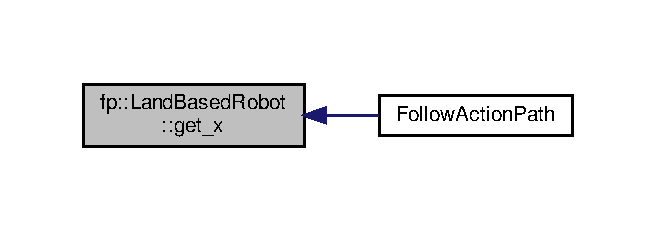
\includegraphics[width=315pt]{classfp_1_1_land_based_robot_a3624c5d041de0987c0103c6b01fa9bc6_icgraph}
\end{center}
\end{figure}
\mbox{\Hypertarget{classfp_1_1_land_based_robot_ae742797bee07ac5b92bfe934cbfed6e9}\label{classfp_1_1_land_based_robot_ae742797bee07ac5b92bfe934cbfed6e9}} 
\index{fp\+::\+Land\+Based\+Robot@{fp\+::\+Land\+Based\+Robot}!get\+\_\+y@{get\+\_\+y}}
\index{get\+\_\+y@{get\+\_\+y}!fp\+::\+Land\+Based\+Robot@{fp\+::\+Land\+Based\+Robot}}
\subsubsection{\texorpdfstring{get\+\_\+y()}{get\_y()}}
{\footnotesize\ttfamily int fp\+::\+Land\+Based\+Robot\+::get\+\_\+y (\begin{DoxyParamCaption}{ }\end{DoxyParamCaption})\hspace{0.3cm}{\ttfamily [pure virtual]}}



This will just ouput that appropriate function are called or not. 

\hypertarget{main_8cpp_Description}{}\subsection{Description}\label{main_8cpp_Description}
F\+U\+N\+C\+T\+I\+ON N\+A\+ME -\/ get\+\_\+y F\+U\+N\+C\+T\+I\+ON P\+A\+R\+A\+M\+E\+T\+ER T\+Y\+PE -\/ none 

Implemented in \hyperlink{classfp_1_1_land_based_wheeled_ae793757fd11ba270a6d9c335acb8cafd}{fp\+::\+Land\+Based\+Wheeled}, and \hyperlink{classfp_1_1_land_based_tracked_a09738928390e7e0d33444b6a7cfcc841}{fp\+::\+Land\+Based\+Tracked}.

Here is the caller graph for this function\+:
\nopagebreak
\begin{figure}[H]
\begin{center}
\leavevmode
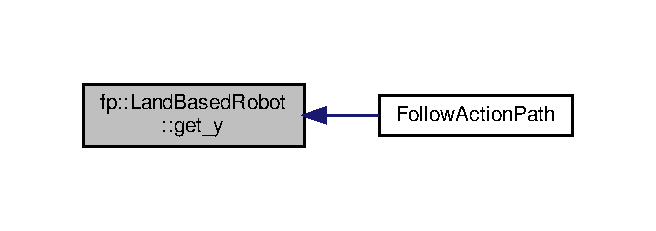
\includegraphics[width=315pt]{classfp_1_1_land_based_robot_ae742797bee07ac5b92bfe934cbfed6e9_icgraph}
\end{center}
\end{figure}
\mbox{\Hypertarget{classfp_1_1_land_based_robot_a50841b6e40d4e92832770d26b427fea2}\label{classfp_1_1_land_based_robot_a50841b6e40d4e92832770d26b427fea2}} 
\index{fp\+::\+Land\+Based\+Robot@{fp\+::\+Land\+Based\+Robot}!Get\+Direction@{Get\+Direction}}
\index{Get\+Direction@{Get\+Direction}!fp\+::\+Land\+Based\+Robot@{fp\+::\+Land\+Based\+Robot}}
\subsubsection{\texorpdfstring{Get\+Direction()}{GetDirection()}}
{\footnotesize\ttfamily char fp\+::\+Land\+Based\+Robot\+::\+Get\+Direction (\begin{DoxyParamCaption}{ }\end{DoxyParamCaption})\hspace{0.3cm}{\ttfamily [pure virtual]}}



This will get direction of robot. 

This is used to get the direction as character form\hypertarget{main_8cpp_Description}{}\subsection{Description}\label{main_8cpp_Description}
F\+U\+N\+C\+T\+I\+ON N\+A\+ME -\/ Get\+\_\+\+Direction F\+U\+N\+C\+T\+I\+ON P\+A\+R\+A\+M\+E\+T\+ER T\+Y\+PE -\/ none 

Implemented in \hyperlink{classfp_1_1_land_based_wheeled_a87c986392b37f25dd63e03866c2ab9c2}{fp\+::\+Land\+Based\+Wheeled}, and \hyperlink{classfp_1_1_land_based_tracked_acb4201d9ba3660fbdb52bc95cddaa5bf}{fp\+::\+Land\+Based\+Tracked}.

\mbox{\Hypertarget{classfp_1_1_land_based_robot_a5df828c5d6c1f7fb4c7b68f53d9c6080}\label{classfp_1_1_land_based_robot_a5df828c5d6c1f7fb4c7b68f53d9c6080}} 
\index{fp\+::\+Land\+Based\+Robot@{fp\+::\+Land\+Based\+Robot}!Move\+Forward@{Move\+Forward}}
\index{Move\+Forward@{Move\+Forward}!fp\+::\+Land\+Based\+Robot@{fp\+::\+Land\+Based\+Robot}}
\subsubsection{\texorpdfstring{Move\+Forward()}{MoveForward()}}
{\footnotesize\ttfamily void fp\+::\+Land\+Based\+Robot\+::\+Move\+Forward (\begin{DoxyParamCaption}{ }\end{DoxyParamCaption})\hspace{0.3cm}{\ttfamily [pure virtual]}}



Implemented in \hyperlink{classfp_1_1_land_based_wheeled_af7875b805655b6f654e49a885f31122a}{fp\+::\+Land\+Based\+Wheeled}, and \hyperlink{classfp_1_1_land_based_tracked_af537a096f507674b62a9691fad7c6cb7}{fp\+::\+Land\+Based\+Tracked}.

Here is the caller graph for this function\+:
\nopagebreak
\begin{figure}[H]
\begin{center}
\leavevmode
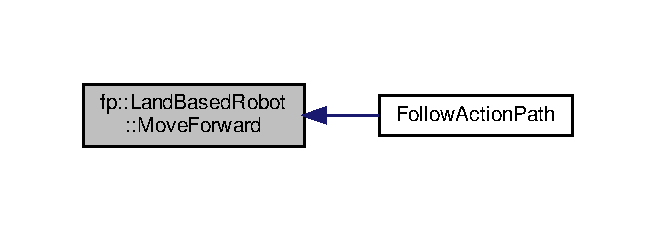
\includegraphics[width=315pt]{classfp_1_1_land_based_robot_a5df828c5d6c1f7fb4c7b68f53d9c6080_icgraph}
\end{center}
\end{figure}
\mbox{\Hypertarget{classfp_1_1_land_based_robot_a359e1012e9093475b7a1b0d38e41a118}\label{classfp_1_1_land_based_robot_a359e1012e9093475b7a1b0d38e41a118}} 
\index{fp\+::\+Land\+Based\+Robot@{fp\+::\+Land\+Based\+Robot}!Turn\+Left@{Turn\+Left}}
\index{Turn\+Left@{Turn\+Left}!fp\+::\+Land\+Based\+Robot@{fp\+::\+Land\+Based\+Robot}}
\subsubsection{\texorpdfstring{Turn\+Left()}{TurnLeft()}}
{\footnotesize\ttfamily void fp\+::\+Land\+Based\+Robot\+::\+Turn\+Left (\begin{DoxyParamCaption}\item[{int}]{x,  }\item[{int}]{y }\end{DoxyParamCaption})\hspace{0.3cm}{\ttfamily [pure virtual]}}



This will just ouput that appropriate function are called or not. 

\hypertarget{main_8cpp_Description}{}\subsection{Description}\label{main_8cpp_Description}
F\+U\+N\+C\+T\+I\+ON N\+A\+ME -\/ Turn\+Left F\+U\+N\+C\+T\+I\+ON P\+A\+R\+A\+M\+E\+T\+ER T\+Y\+PE -\/ two integers 

Implemented in \hyperlink{classfp_1_1_land_based_wheeled_a2f2434db907aaef26b8f3084e84b3579}{fp\+::\+Land\+Based\+Wheeled}, and \hyperlink{classfp_1_1_land_based_tracked_aab40e1a48e5142491f02b2936c4cacc3}{fp\+::\+Land\+Based\+Tracked}.

Here is the caller graph for this function\+:
\nopagebreak
\begin{figure}[H]
\begin{center}
\leavevmode
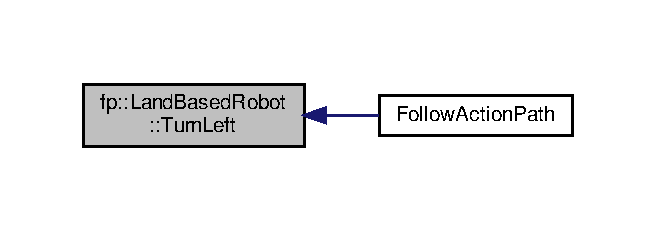
\includegraphics[width=315pt]{classfp_1_1_land_based_robot_a359e1012e9093475b7a1b0d38e41a118_icgraph}
\end{center}
\end{figure}
\mbox{\Hypertarget{classfp_1_1_land_based_robot_a7360e4084bc5254f72ab0d3612644907}\label{classfp_1_1_land_based_robot_a7360e4084bc5254f72ab0d3612644907}} 
\index{fp\+::\+Land\+Based\+Robot@{fp\+::\+Land\+Based\+Robot}!Turn\+Right@{Turn\+Right}}
\index{Turn\+Right@{Turn\+Right}!fp\+::\+Land\+Based\+Robot@{fp\+::\+Land\+Based\+Robot}}
\subsubsection{\texorpdfstring{Turn\+Right()}{TurnRight()}}
{\footnotesize\ttfamily void fp\+::\+Land\+Based\+Robot\+::\+Turn\+Right (\begin{DoxyParamCaption}\item[{int}]{x,  }\item[{int}]{y }\end{DoxyParamCaption})\hspace{0.3cm}{\ttfamily [pure virtual]}}



This will just ouput that appropriate function are called or not. 

\hypertarget{main_8cpp_Description}{}\subsection{Description}\label{main_8cpp_Description}
F\+U\+N\+C\+T\+I\+ON N\+A\+ME -\/ Turn\+Right F\+U\+N\+C\+T\+I\+ON P\+A\+R\+A\+M\+E\+T\+ER T\+Y\+PE -\/ two integers 

Implemented in \hyperlink{classfp_1_1_land_based_wheeled_ac6e93b00e624e281a497e99729db04e7}{fp\+::\+Land\+Based\+Wheeled}, and \hyperlink{classfp_1_1_land_based_tracked_a619c29950f6c484d3481e31ff01dad3a}{fp\+::\+Land\+Based\+Tracked}.

Here is the caller graph for this function\+:
\nopagebreak
\begin{figure}[H]
\begin{center}
\leavevmode
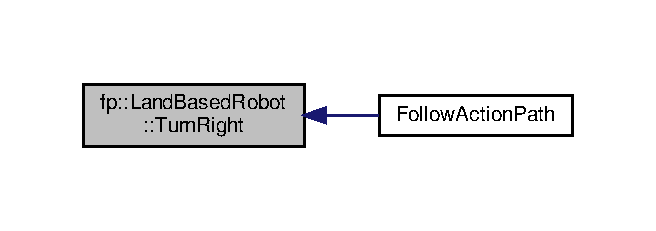
\includegraphics[width=315pt]{classfp_1_1_land_based_robot_a7360e4084bc5254f72ab0d3612644907_icgraph}
\end{center}
\end{figure}


\subsection{Member Data Documentation}
\mbox{\Hypertarget{classfp_1_1_land_based_robot_a542d90c7c62899e3c3cf28791bbb6c8e}\label{classfp_1_1_land_based_robot_a542d90c7c62899e3c3cf28791bbb6c8e}} 
\index{fp\+::\+Land\+Based\+Robot@{fp\+::\+Land\+Based\+Robot}!capacity\+\_\+@{capacity\+\_\+}}
\index{capacity\+\_\+@{capacity\+\_\+}!fp\+::\+Land\+Based\+Robot@{fp\+::\+Land\+Based\+Robot}}
\subsubsection{\texorpdfstring{capacity\+\_\+}{capacity\_}}
{\footnotesize\ttfamily double fp\+::\+Land\+Based\+Robot\+::capacity\+\_\+\hspace{0.3cm}{\ttfamily [protected]}}

capaity of robot \mbox{\Hypertarget{classfp_1_1_land_based_robot_adc8e6123fa8ffe86576e46000b0ae779}\label{classfp_1_1_land_based_robot_adc8e6123fa8ffe86576e46000b0ae779}} 
\index{fp\+::\+Land\+Based\+Robot@{fp\+::\+Land\+Based\+Robot}!direction\+\_\+@{direction\+\_\+}}
\index{direction\+\_\+@{direction\+\_\+}!fp\+::\+Land\+Based\+Robot@{fp\+::\+Land\+Based\+Robot}}
\subsubsection{\texorpdfstring{direction\+\_\+}{direction\_}}
{\footnotesize\ttfamily char fp\+::\+Land\+Based\+Robot\+::direction\+\_\+\hspace{0.3cm}{\ttfamily [protected]}}

direction of robot \mbox{\Hypertarget{classfp_1_1_land_based_robot_a34238a27d9055c416a3e6cfedc8ed248}\label{classfp_1_1_land_based_robot_a34238a27d9055c416a3e6cfedc8ed248}} 
\index{fp\+::\+Land\+Based\+Robot@{fp\+::\+Land\+Based\+Robot}!height\+\_\+@{height\+\_\+}}
\index{height\+\_\+@{height\+\_\+}!fp\+::\+Land\+Based\+Robot@{fp\+::\+Land\+Based\+Robot}}
\subsubsection{\texorpdfstring{height\+\_\+}{height\_}}
{\footnotesize\ttfamily double fp\+::\+Land\+Based\+Robot\+::height\+\_\+\hspace{0.3cm}{\ttfamily [protected]}}

height attribut of robot \mbox{\Hypertarget{classfp_1_1_land_based_robot_a9475d5886f329c92e68f0d86b4da58c0}\label{classfp_1_1_land_based_robot_a9475d5886f329c92e68f0d86b4da58c0}} 
\index{fp\+::\+Land\+Based\+Robot@{fp\+::\+Land\+Based\+Robot}!length\+\_\+@{length\+\_\+}}
\index{length\+\_\+@{length\+\_\+}!fp\+::\+Land\+Based\+Robot@{fp\+::\+Land\+Based\+Robot}}
\subsubsection{\texorpdfstring{length\+\_\+}{length\_}}
{\footnotesize\ttfamily double fp\+::\+Land\+Based\+Robot\+::length\+\_\+\hspace{0.3cm}{\ttfamily [protected]}}

length attribut of robot \mbox{\Hypertarget{classfp_1_1_land_based_robot_ac79ca2c52e99bc96534bb7a57dcb9030}\label{classfp_1_1_land_based_robot_ac79ca2c52e99bc96534bb7a57dcb9030}} 
\index{fp\+::\+Land\+Based\+Robot@{fp\+::\+Land\+Based\+Robot}!name\+\_\+@{name\+\_\+}}
\index{name\+\_\+@{name\+\_\+}!fp\+::\+Land\+Based\+Robot@{fp\+::\+Land\+Based\+Robot}}
\subsubsection{\texorpdfstring{name\+\_\+}{name\_}}
{\footnotesize\ttfamily std\+::string fp\+::\+Land\+Based\+Robot\+::name\+\_\+\hspace{0.3cm}{\ttfamily [protected]}}

protected name of the robot \mbox{\Hypertarget{classfp_1_1_land_based_robot_ae969157e5f910ed0a85198dc7f6c3cef}\label{classfp_1_1_land_based_robot_ae969157e5f910ed0a85198dc7f6c3cef}} 
\index{fp\+::\+Land\+Based\+Robot@{fp\+::\+Land\+Based\+Robot}!speed\+\_\+@{speed\+\_\+}}
\index{speed\+\_\+@{speed\+\_\+}!fp\+::\+Land\+Based\+Robot@{fp\+::\+Land\+Based\+Robot}}
\subsubsection{\texorpdfstring{speed\+\_\+}{speed\_}}
{\footnotesize\ttfamily double fp\+::\+Land\+Based\+Robot\+::speed\+\_\+\hspace{0.3cm}{\ttfamily [protected]}}

a float speed of robot \mbox{\Hypertarget{classfp_1_1_land_based_robot_aae605323e9ce63f29dcded204421b1fc}\label{classfp_1_1_land_based_robot_aae605323e9ce63f29dcded204421b1fc}} 
\index{fp\+::\+Land\+Based\+Robot@{fp\+::\+Land\+Based\+Robot}!width\+\_\+@{width\+\_\+}}
\index{width\+\_\+@{width\+\_\+}!fp\+::\+Land\+Based\+Robot@{fp\+::\+Land\+Based\+Robot}}
\subsubsection{\texorpdfstring{width\+\_\+}{width\_}}
{\footnotesize\ttfamily double fp\+::\+Land\+Based\+Robot\+::width\+\_\+\hspace{0.3cm}{\ttfamily [protected]}}

width of robot \mbox{\Hypertarget{classfp_1_1_land_based_robot_a55c2b5865fd60fb0158a135031f8b271}\label{classfp_1_1_land_based_robot_a55c2b5865fd60fb0158a135031f8b271}} 
\index{fp\+::\+Land\+Based\+Robot@{fp\+::\+Land\+Based\+Robot}!x\+\_\+@{x\+\_\+}}
\index{x\+\_\+@{x\+\_\+}!fp\+::\+Land\+Based\+Robot@{fp\+::\+Land\+Based\+Robot}}
\subsubsection{\texorpdfstring{x\+\_\+}{x\_}}
{\footnotesize\ttfamily int fp\+::\+Land\+Based\+Robot\+::x\+\_\+\hspace{0.3cm}{\ttfamily [protected]}}

X-\/\+Co-\/ordinate of robot location \mbox{\Hypertarget{classfp_1_1_land_based_robot_a130cfd6ad383116076dc891ee3a52671}\label{classfp_1_1_land_based_robot_a130cfd6ad383116076dc891ee3a52671}} 
\index{fp\+::\+Land\+Based\+Robot@{fp\+::\+Land\+Based\+Robot}!y\+\_\+@{y\+\_\+}}
\index{y\+\_\+@{y\+\_\+}!fp\+::\+Land\+Based\+Robot@{fp\+::\+Land\+Based\+Robot}}
\subsubsection{\texorpdfstring{y\+\_\+}{y\_}}
{\footnotesize\ttfamily int fp\+::\+Land\+Based\+Robot\+::y\+\_\+\hspace{0.3cm}{\ttfamily [protected]}}

Y-\/\+Co-\/ordinate of robot location 

The documentation for this class was generated from the following files\+:\begin{DoxyCompactItemize}
\item 
src/\+Land\+Based\+Robot/\hyperlink{_land_based_robot_8h}{Land\+Based\+Robot.\+h}\item 
src/\+Land\+Based\+Robot/\hyperlink{_land_based_robot_8cpp}{Land\+Based\+Robot.\+cpp}\end{DoxyCompactItemize}

\hypertarget{class_landbased_robot}{}\section{Landbased\+Robot Class Reference}
\label{class_landbased_robot}\index{Landbased\+Robot@{Landbased\+Robot}}


{\ttfamily \#include $<$Land\+Based\+Robot.\+h$>$}



\subsection{Detailed Description}
\begin{DoxyAuthor}{Author}
Group-\/9-\/\+E\+N\+P\+M809Y 
\end{DoxyAuthor}
\begin{DoxyDate}{Date}
03/12/19 
\end{DoxyDate}


The documentation for this class was generated from the following file\+:\begin{DoxyCompactItemize}
\item 
src/\+Land\+Based\+Robot/\hyperlink{_land_based_robot_8h}{Land\+Based\+Robot.\+h}\end{DoxyCompactItemize}

\hypertarget{classfp_1_1_land_based_tracked}{}\section{fp\+:\+:Land\+Based\+Tracked Class Reference}
\label{classfp_1_1_land_based_tracked}\index{fp\+::\+Land\+Based\+Tracked@{fp\+::\+Land\+Based\+Tracked}}


A Landbased\+Tracked class..  




{\ttfamily \#include $<$Land\+Based\+Tracked.\+h$>$}



Inheritance diagram for fp\+:\+:Land\+Based\+Tracked\+:
\nopagebreak
\begin{figure}[H]
\begin{center}
\leavevmode
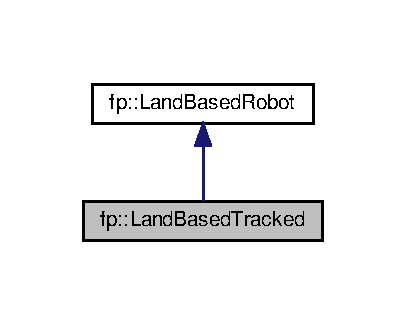
\includegraphics[width=195pt]{classfp_1_1_land_based_tracked__inherit__graph}
\end{center}
\end{figure}


Collaboration diagram for fp\+:\+:Land\+Based\+Tracked\+:
\nopagebreak
\begin{figure}[H]
\begin{center}
\leavevmode
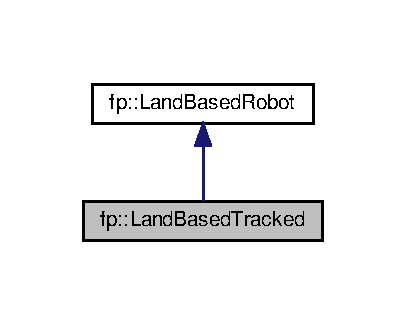
\includegraphics[width=195pt]{classfp_1_1_land_based_tracked__coll__graph}
\end{center}
\end{figure}
\subsection*{Public Member Functions}
\begin{DoxyCompactItemize}
\item 
\hyperlink{classfp_1_1_land_based_tracked_a165b455a487d13eddfd5f015bc579b95}{Land\+Based\+Tracked} (std\+::string name, int x, int y)
\item 
\hyperlink{classfp_1_1_land_based_tracked_a0f9489dc8ef0310ced4f2526a610a0e0}{Land\+Based\+Tracked} ()
\item 
virtual \hyperlink{classfp_1_1_land_based_tracked_a8d3033324bbc96fde30ce107c1694af3}{$\sim$\+Land\+Based\+Tracked} ()
\item 
virtual void \hyperlink{classfp_1_1_land_based_tracked_af537a096f507674b62a9691fad7c6cb7}{Move\+Forward} () override
\begin{DoxyCompactList}\small\item\em This will move forward. \end{DoxyCompactList}\item 
virtual void \hyperlink{classfp_1_1_land_based_tracked_aab40e1a48e5142491f02b2936c4cacc3}{Turn\+Left} (int, int) override
\begin{DoxyCompactList}\small\item\em This function works for Turnleft for tracked robot. \end{DoxyCompactList}\item 
virtual void \hyperlink{classfp_1_1_land_based_tracked_a619c29950f6c484d3481e31ff01dad3a}{Turn\+Right} (int, int) override
\begin{DoxyCompactList}\small\item\em This function works for Turn\+Right for tracked robot. \end{DoxyCompactList}\item 
virtual int \hyperlink{classfp_1_1_land_based_tracked_a3a4fc3c84dd3fcf1928a27af1658680f}{get\+\_\+x} () override
\begin{DoxyCompactList}\small\item\em This function works as getter for x coordinate. \end{DoxyCompactList}\item 
virtual int \hyperlink{classfp_1_1_land_based_tracked_a09738928390e7e0d33444b6a7cfcc841}{get\+\_\+y} () override
\begin{DoxyCompactList}\small\item\em This function works as getter for y coordinate. \end{DoxyCompactList}\item 
virtual char \hyperlink{classfp_1_1_land_based_tracked_acb4201d9ba3660fbdb52bc95cddaa5bf}{Get\+Direction} () override
\begin{DoxyCompactList}\small\item\em This function is getter function for direction. \end{DoxyCompactList}\item 
virtual double \hyperlink{classfp_1_1_land_based_tracked_a5c5c280d150b040bd5f862f2f64d83f1}{get\+\_\+speed} () override
\begin{DoxyCompactList}\small\item\em This function is getter function for spped. \end{DoxyCompactList}\end{DoxyCompactItemize}
\subsection*{Protected Attributes}
\begin{DoxyCompactItemize}
\item 
std\+::string \hyperlink{classfp_1_1_land_based_tracked_a89923d6f493b1581a882f531ed6de3ea}{track\+\_\+type}
\end{DoxyCompactItemize}


\subsection{Detailed Description}
A Landbased\+Tracked class.. 

This class is derived from from the \hyperlink{classfp_1_1_land_based_robot}{Land\+Based\+Robot} base class and it has access to every member function of base class. 

\subsection{Constructor \& Destructor Documentation}
\mbox{\Hypertarget{classfp_1_1_land_based_tracked_a165b455a487d13eddfd5f015bc579b95}\label{classfp_1_1_land_based_tracked_a165b455a487d13eddfd5f015bc579b95}} 
\index{fp\+::\+Land\+Based\+Tracked@{fp\+::\+Land\+Based\+Tracked}!Land\+Based\+Tracked@{Land\+Based\+Tracked}}
\index{Land\+Based\+Tracked@{Land\+Based\+Tracked}!fp\+::\+Land\+Based\+Tracked@{fp\+::\+Land\+Based\+Tracked}}
\subsubsection{\texorpdfstring{Land\+Based\+Tracked()}{LandBasedTracked()}\hspace{0.1cm}{\footnotesize\ttfamily [1/2]}}
{\footnotesize\ttfamily fp\+::\+Land\+Based\+Tracked\+::\+Land\+Based\+Tracked (\begin{DoxyParamCaption}\item[{std\+::string}]{name,  }\item[{int}]{x,  }\item[{int}]{y }\end{DoxyParamCaption})}

A constructor. A constructor which takes name and x and y as an argument.

A constructor. A constructor which takes name, x, and y as arguments and sets these parameters. \mbox{\Hypertarget{classfp_1_1_land_based_tracked_a0f9489dc8ef0310ced4f2526a610a0e0}\label{classfp_1_1_land_based_tracked_a0f9489dc8ef0310ced4f2526a610a0e0}} 
\index{fp\+::\+Land\+Based\+Tracked@{fp\+::\+Land\+Based\+Tracked}!Land\+Based\+Tracked@{Land\+Based\+Tracked}}
\index{Land\+Based\+Tracked@{Land\+Based\+Tracked}!fp\+::\+Land\+Based\+Tracked@{fp\+::\+Land\+Based\+Tracked}}
\subsubsection{\texorpdfstring{Land\+Based\+Tracked()}{LandBasedTracked()}\hspace{0.1cm}{\footnotesize\ttfamily [2/2]}}
{\footnotesize\ttfamily fp\+::\+Land\+Based\+Tracked\+::\+Land\+Based\+Tracked (\begin{DoxyParamCaption}{ }\end{DoxyParamCaption})}

A constructor. A constructor with no arguments.

A constructor. A constructor which takes no arguments and initializes name to none and x \& y to 0. \mbox{\Hypertarget{classfp_1_1_land_based_tracked_a8d3033324bbc96fde30ce107c1694af3}\label{classfp_1_1_land_based_tracked_a8d3033324bbc96fde30ce107c1694af3}} 
\index{fp\+::\+Land\+Based\+Tracked@{fp\+::\+Land\+Based\+Tracked}!````~Land\+Based\+Tracked@{$\sim$\+Land\+Based\+Tracked}}
\index{````~Land\+Based\+Tracked@{$\sim$\+Land\+Based\+Tracked}!fp\+::\+Land\+Based\+Tracked@{fp\+::\+Land\+Based\+Tracked}}
\subsubsection{\texorpdfstring{$\sim$\+Land\+Based\+Tracked()}{~LandBasedTracked()}}
{\footnotesize\ttfamily fp\+::\+Land\+Based\+Tracked\+::$\sim$\+Land\+Based\+Tracked (\begin{DoxyParamCaption}{ }\end{DoxyParamCaption})\hspace{0.3cm}{\ttfamily [virtual]}}

A destructor. This will destroy the object \hyperlink{classfp_1_1_land_based_tracked}{Land\+Based\+Tracked} after use 

\subsection{Member Function Documentation}
\mbox{\Hypertarget{classfp_1_1_land_based_tracked_a5c5c280d150b040bd5f862f2f64d83f1}\label{classfp_1_1_land_based_tracked_a5c5c280d150b040bd5f862f2f64d83f1}} 
\index{fp\+::\+Land\+Based\+Tracked@{fp\+::\+Land\+Based\+Tracked}!get\+\_\+speed@{get\+\_\+speed}}
\index{get\+\_\+speed@{get\+\_\+speed}!fp\+::\+Land\+Based\+Tracked@{fp\+::\+Land\+Based\+Tracked}}
\subsubsection{\texorpdfstring{get\+\_\+speed()}{get\_speed()}}
{\footnotesize\ttfamily virtual double fp\+::\+Land\+Based\+Tracked\+::get\+\_\+speed (\begin{DoxyParamCaption}{ }\end{DoxyParamCaption})\hspace{0.3cm}{\ttfamily [inline]}, {\ttfamily [override]}, {\ttfamily [virtual]}}



This function is getter function for spped. 


\begin{DoxyParams}{Parameters}
{\em None} & \\
\hline
\end{DoxyParams}
\begin{DoxyReturn}{Returns}
char 
\end{DoxyReturn}
\hypertarget{_m_a_z_e_8h_DESCRIPTION}{}\subsection{D\+E\+S\+C\+R\+I\+P\+T\+I\+ON}\label{_m_a_z_e_8h_DESCRIPTION}
F\+U\+N\+C\+T\+I\+ON N\+A\+ME -\/ \hyperlink{classfp_1_1_land_based_tracked_a5c5c280d150b040bd5f862f2f64d83f1}{get\+\_\+speed()} F\+U\+N\+C\+T\+I\+ON P\+A\+R\+A\+M\+E\+T\+ER T\+Y\+PE -\/ char R\+E\+T\+U\+RN T\+Y\+PE OF \hyperlink{classfp_1_1_land_based_tracked_a09738928390e7e0d33444b6a7cfcc841}{get\+\_\+y()} is char. 

Implements \hyperlink{classfp_1_1_land_based_robot_a68844e9c442d1b293945144dc6c6608c}{fp\+::\+Land\+Based\+Robot}.

\mbox{\Hypertarget{classfp_1_1_land_based_tracked_a3a4fc3c84dd3fcf1928a27af1658680f}\label{classfp_1_1_land_based_tracked_a3a4fc3c84dd3fcf1928a27af1658680f}} 
\index{fp\+::\+Land\+Based\+Tracked@{fp\+::\+Land\+Based\+Tracked}!get\+\_\+x@{get\+\_\+x}}
\index{get\+\_\+x@{get\+\_\+x}!fp\+::\+Land\+Based\+Tracked@{fp\+::\+Land\+Based\+Tracked}}
\subsubsection{\texorpdfstring{get\+\_\+x()}{get\_x()}}
{\footnotesize\ttfamily virtual int fp\+::\+Land\+Based\+Tracked\+::get\+\_\+x (\begin{DoxyParamCaption}{ }\end{DoxyParamCaption})\hspace{0.3cm}{\ttfamily [inline]}, {\ttfamily [override]}, {\ttfamily [virtual]}}



This function works as getter for x coordinate. 


\begin{DoxyParams}{Parameters}
{\em None} & \\
\hline
\end{DoxyParams}
\begin{DoxyReturn}{Returns}
int 
\end{DoxyReturn}
\hypertarget{_m_a_z_e_8h_DESCRIPTION}{}\subsection{D\+E\+S\+C\+R\+I\+P\+T\+I\+ON}\label{_m_a_z_e_8h_DESCRIPTION}
F\+U\+N\+C\+T\+I\+ON N\+A\+ME -\/ \hyperlink{classfp_1_1_land_based_tracked_a3a4fc3c84dd3fcf1928a27af1658680f}{get\+\_\+x()} F\+U\+N\+C\+T\+I\+ON P\+A\+R\+A\+M\+E\+T\+ER T\+Y\+PE -\/ void R\+E\+T\+U\+RN T\+Y\+PE OF \hyperlink{classfp_1_1_land_based_tracked_a3a4fc3c84dd3fcf1928a27af1658680f}{get\+\_\+x()} is integer. 

Implements \hyperlink{classfp_1_1_land_based_robot_a3624c5d041de0987c0103c6b01fa9bc6}{fp\+::\+Land\+Based\+Robot}.

\mbox{\Hypertarget{classfp_1_1_land_based_tracked_a09738928390e7e0d33444b6a7cfcc841}\label{classfp_1_1_land_based_tracked_a09738928390e7e0d33444b6a7cfcc841}} 
\index{fp\+::\+Land\+Based\+Tracked@{fp\+::\+Land\+Based\+Tracked}!get\+\_\+y@{get\+\_\+y}}
\index{get\+\_\+y@{get\+\_\+y}!fp\+::\+Land\+Based\+Tracked@{fp\+::\+Land\+Based\+Tracked}}
\subsubsection{\texorpdfstring{get\+\_\+y()}{get\_y()}}
{\footnotesize\ttfamily virtual int fp\+::\+Land\+Based\+Tracked\+::get\+\_\+y (\begin{DoxyParamCaption}{ }\end{DoxyParamCaption})\hspace{0.3cm}{\ttfamily [inline]}, {\ttfamily [override]}, {\ttfamily [virtual]}}



This function works as getter for y coordinate. 


\begin{DoxyParams}{Parameters}
{\em None} & \\
\hline
\end{DoxyParams}
\begin{DoxyReturn}{Returns}
integer 
\end{DoxyReturn}
\hypertarget{_m_a_z_e_8h_DESCRIPTION}{}\subsection{D\+E\+S\+C\+R\+I\+P\+T\+I\+ON}\label{_m_a_z_e_8h_DESCRIPTION}
F\+U\+N\+C\+T\+I\+ON N\+A\+ME -\/ \hyperlink{classfp_1_1_land_based_tracked_a09738928390e7e0d33444b6a7cfcc841}{get\+\_\+y()} F\+U\+N\+C\+T\+I\+ON P\+A\+R\+A\+M\+E\+T\+ER T\+Y\+PE -\/ void R\+E\+T\+U\+RN T\+Y\+PE OF \hyperlink{classfp_1_1_land_based_tracked_a09738928390e7e0d33444b6a7cfcc841}{get\+\_\+y()} is integer. 

Implements \hyperlink{classfp_1_1_land_based_robot_ae742797bee07ac5b92bfe934cbfed6e9}{fp\+::\+Land\+Based\+Robot}.

\mbox{\Hypertarget{classfp_1_1_land_based_tracked_acb4201d9ba3660fbdb52bc95cddaa5bf}\label{classfp_1_1_land_based_tracked_acb4201d9ba3660fbdb52bc95cddaa5bf}} 
\index{fp\+::\+Land\+Based\+Tracked@{fp\+::\+Land\+Based\+Tracked}!Get\+Direction@{Get\+Direction}}
\index{Get\+Direction@{Get\+Direction}!fp\+::\+Land\+Based\+Tracked@{fp\+::\+Land\+Based\+Tracked}}
\subsubsection{\texorpdfstring{Get\+Direction()}{GetDirection()}}
{\footnotesize\ttfamily virtual char fp\+::\+Land\+Based\+Tracked\+::\+Get\+Direction (\begin{DoxyParamCaption}{ }\end{DoxyParamCaption})\hspace{0.3cm}{\ttfamily [inline]}, {\ttfamily [override]}, {\ttfamily [virtual]}}



This function is getter function for direction. 


\begin{DoxyParams}{Parameters}
{\em None} & \\
\hline
\end{DoxyParams}
\begin{DoxyReturn}{Returns}
char 
\end{DoxyReturn}
\hypertarget{_m_a_z_e_8h_DESCRIPTION}{}\subsection{D\+E\+S\+C\+R\+I\+P\+T\+I\+ON}\label{_m_a_z_e_8h_DESCRIPTION}
F\+U\+N\+C\+T\+I\+ON N\+A\+ME -\/ get\+\_\+\+Direction() F\+U\+N\+C\+T\+I\+ON P\+A\+R\+A\+M\+E\+T\+ER T\+Y\+PE -\/ char R\+E\+T\+U\+RN T\+Y\+PE OF \hyperlink{classfp_1_1_land_based_tracked_a09738928390e7e0d33444b6a7cfcc841}{get\+\_\+y()} is char. 

Implements \hyperlink{classfp_1_1_land_based_robot_a50841b6e40d4e92832770d26b427fea2}{fp\+::\+Land\+Based\+Robot}.

\mbox{\Hypertarget{classfp_1_1_land_based_tracked_af537a096f507674b62a9691fad7c6cb7}\label{classfp_1_1_land_based_tracked_af537a096f507674b62a9691fad7c6cb7}} 
\index{fp\+::\+Land\+Based\+Tracked@{fp\+::\+Land\+Based\+Tracked}!Move\+Forward@{Move\+Forward}}
\index{Move\+Forward@{Move\+Forward}!fp\+::\+Land\+Based\+Tracked@{fp\+::\+Land\+Based\+Tracked}}
\subsubsection{\texorpdfstring{Move\+Forward()}{MoveForward()}}
{\footnotesize\ttfamily void fp\+::\+Land\+Based\+Tracked\+::\+Move\+Forward (\begin{DoxyParamCaption}{ }\end{DoxyParamCaption})\hspace{0.3cm}{\ttfamily [override]}, {\ttfamily [virtual]}}



This will move forward. 

\hypertarget{main_8cpp_Description}{}\subsection{Description}\label{main_8cpp_Description}
F\+U\+N\+C\+T\+I\+ON N\+A\+ME -\/ Move\+Forward F\+U\+N\+C\+T\+I\+ON P\+A\+R\+A\+M\+E\+T\+ER T\+Y\+PE -\/ two integers 

Implements \hyperlink{classfp_1_1_land_based_robot_a5df828c5d6c1f7fb4c7b68f53d9c6080}{fp\+::\+Land\+Based\+Robot}.

\mbox{\Hypertarget{classfp_1_1_land_based_tracked_aab40e1a48e5142491f02b2936c4cacc3}\label{classfp_1_1_land_based_tracked_aab40e1a48e5142491f02b2936c4cacc3}} 
\index{fp\+::\+Land\+Based\+Tracked@{fp\+::\+Land\+Based\+Tracked}!Turn\+Left@{Turn\+Left}}
\index{Turn\+Left@{Turn\+Left}!fp\+::\+Land\+Based\+Tracked@{fp\+::\+Land\+Based\+Tracked}}
\subsubsection{\texorpdfstring{Turn\+Left()}{TurnLeft()}}
{\footnotesize\ttfamily void fp\+::\+Land\+Based\+Tracked\+::\+Turn\+Left (\begin{DoxyParamCaption}\item[{int}]{x,  }\item[{int}]{y }\end{DoxyParamCaption})\hspace{0.3cm}{\ttfamily [override]}, {\ttfamily [virtual]}}



This function works for Turnleft for tracked robot. 

This will turn robot left given as co-\/ordinates.


\begin{DoxyParams}{Parameters}
{\em int} & \\
\hline
{\em int} & \\
\hline
\end{DoxyParams}
\begin{DoxyReturn}{Returns}
none 
\end{DoxyReturn}
\hypertarget{_m_a_z_e_8h_DESCRIPTION}{}\subsection{D\+E\+S\+C\+R\+I\+P\+T\+I\+ON}\label{_m_a_z_e_8h_DESCRIPTION}
F\+U\+N\+C\+T\+I\+ON N\+A\+ME -\/ \hyperlink{classfp_1_1_land_based_tracked_aab40e1a48e5142491f02b2936c4cacc3}{Turn\+Left()} F\+U\+N\+C\+T\+I\+ON P\+A\+R\+A\+M\+E\+T\+ER T\+Y\+PE -\/ integers R\+E\+T\+U\+RN T\+Y\+PE OF \hyperlink{classfp_1_1_land_based_tracked_aab40e1a48e5142491f02b2936c4cacc3}{Turn\+Left()} is void.\hypertarget{main_8cpp_Description}{}\subsection{Description}\label{main_8cpp_Description}
F\+U\+N\+C\+T\+I\+ON N\+A\+ME -\/ Turn\+Left F\+U\+N\+C\+T\+I\+ON P\+A\+R\+A\+M\+E\+T\+ER T\+Y\+PE -\/ two integers 

Implements \hyperlink{classfp_1_1_land_based_robot_a359e1012e9093475b7a1b0d38e41a118}{fp\+::\+Land\+Based\+Robot}.

\mbox{\Hypertarget{classfp_1_1_land_based_tracked_a619c29950f6c484d3481e31ff01dad3a}\label{classfp_1_1_land_based_tracked_a619c29950f6c484d3481e31ff01dad3a}} 
\index{fp\+::\+Land\+Based\+Tracked@{fp\+::\+Land\+Based\+Tracked}!Turn\+Right@{Turn\+Right}}
\index{Turn\+Right@{Turn\+Right}!fp\+::\+Land\+Based\+Tracked@{fp\+::\+Land\+Based\+Tracked}}
\subsubsection{\texorpdfstring{Turn\+Right()}{TurnRight()}}
{\footnotesize\ttfamily void fp\+::\+Land\+Based\+Tracked\+::\+Turn\+Right (\begin{DoxyParamCaption}\item[{int}]{x,  }\item[{int}]{y }\end{DoxyParamCaption})\hspace{0.3cm}{\ttfamily [override]}, {\ttfamily [virtual]}}



This function works for Turn\+Right for tracked robot. 

This will just ouput that appropriate function are called or not.


\begin{DoxyParams}{Parameters}
{\em int} & \\
\hline
{\em int} & \\
\hline
\end{DoxyParams}
\begin{DoxyReturn}{Returns}
none 
\end{DoxyReturn}
\hypertarget{_m_a_z_e_8h_DESCRIPTION}{}\subsection{D\+E\+S\+C\+R\+I\+P\+T\+I\+ON}\label{_m_a_z_e_8h_DESCRIPTION}
F\+U\+N\+C\+T\+I\+ON N\+A\+ME -\/ \hyperlink{classfp_1_1_land_based_tracked_a619c29950f6c484d3481e31ff01dad3a}{Turn\+Right()} F\+U\+N\+C\+T\+I\+ON P\+A\+R\+A\+M\+E\+T\+ER T\+Y\+PE -\/ integers R\+E\+T\+U\+RN T\+Y\+PE OF \hyperlink{classfp_1_1_land_based_tracked_a619c29950f6c484d3481e31ff01dad3a}{Turn\+Right()} is void.\hypertarget{main_8cpp_Description}{}\subsection{Description}\label{main_8cpp_Description}
F\+U\+N\+C\+T\+I\+ON N\+A\+ME -\/ Turn\+Right F\+U\+N\+C\+T\+I\+ON P\+A\+R\+A\+M\+E\+T\+ER T\+Y\+PE -\/ two integers 

Implements \hyperlink{classfp_1_1_land_based_robot_a7360e4084bc5254f72ab0d3612644907}{fp\+::\+Land\+Based\+Robot}.



\subsection{Member Data Documentation}
\mbox{\Hypertarget{classfp_1_1_land_based_tracked_a89923d6f493b1581a882f531ed6de3ea}\label{classfp_1_1_land_based_tracked_a89923d6f493b1581a882f531ed6de3ea}} 
\index{fp\+::\+Land\+Based\+Tracked@{fp\+::\+Land\+Based\+Tracked}!track\+\_\+type@{track\+\_\+type}}
\index{track\+\_\+type@{track\+\_\+type}!fp\+::\+Land\+Based\+Tracked@{fp\+::\+Land\+Based\+Tracked}}
\subsubsection{\texorpdfstring{track\+\_\+type}{track\_type}}
{\footnotesize\ttfamily std\+::string fp\+::\+Land\+Based\+Tracked\+::track\+\_\+type\hspace{0.3cm}{\ttfamily [protected]}}



The documentation for this class was generated from the following files\+:\begin{DoxyCompactItemize}
\item 
src/\+Land\+Based\+Tracked/\hyperlink{_land_based_tracked_8h}{Land\+Based\+Tracked.\+h}\item 
src/\+Land\+Based\+Tracked/\hyperlink{_land_based_tracked_8cpp}{Land\+Based\+Tracked.\+cpp}\end{DoxyCompactItemize}

\hypertarget{classfp_1_1_land_based_wheeled}{}\section{fp\+:\+:Land\+Based\+Wheeled Class Reference}
\label{classfp_1_1_land_based_wheeled}\index{fp\+::\+Land\+Based\+Wheeled@{fp\+::\+Land\+Based\+Wheeled}}


A Landbased\+Wheeled class..  




{\ttfamily \#include $<$Land\+Based\+Wheeled.\+h$>$}



Inheritance diagram for fp\+:\+:Land\+Based\+Wheeled\+:
\nopagebreak
\begin{figure}[H]
\begin{center}
\leavevmode
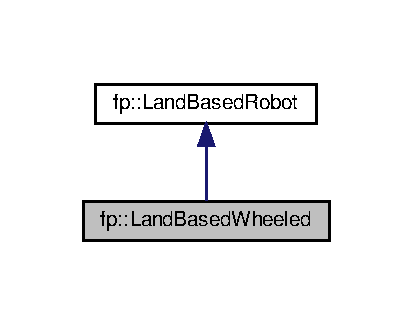
\includegraphics[width=198pt]{classfp_1_1_land_based_wheeled__inherit__graph}
\end{center}
\end{figure}


Collaboration diagram for fp\+:\+:Land\+Based\+Wheeled\+:
\nopagebreak
\begin{figure}[H]
\begin{center}
\leavevmode
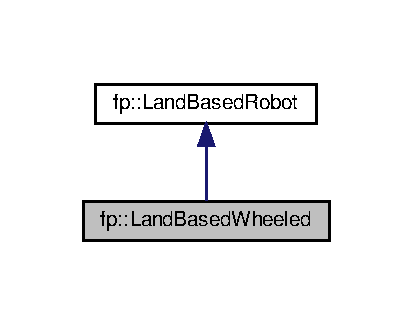
\includegraphics[width=198pt]{classfp_1_1_land_based_wheeled__coll__graph}
\end{center}
\end{figure}
\subsection*{Public Member Functions}
\begin{DoxyCompactItemize}
\item 
\hyperlink{classfp_1_1_land_based_wheeled_ad2b73f9998381dafa6b4a0388acfc28c}{Land\+Based\+Wheeled} (std\+::string name, int x, int y)
\item 
\hyperlink{classfp_1_1_land_based_wheeled_a83884c16bfa5a6153958fd75d509123b}{Land\+Based\+Wheeled} ()
\item 
virtual \hyperlink{classfp_1_1_land_based_wheeled_a87d1d6bf36315ef9dbc79750a968fa2e}{$\sim$\+Land\+Based\+Wheeled} ()
\item 
void \hyperlink{classfp_1_1_land_based_wheeled_a8fc1115e4c49fec71b38a520df4d1528}{Speed\+Up} (int)
\begin{DoxyCompactList}\small\item\em This function works for Speed\+Up for wheeled robot. \end{DoxyCompactList}\item 
virtual void \hyperlink{classfp_1_1_land_based_wheeled_af7875b805655b6f654e49a885f31122a}{Move\+Forward} () override
\item 
virtual void \hyperlink{classfp_1_1_land_based_wheeled_a2f2434db907aaef26b8f3084e84b3579}{Turn\+Left} (int, int) override
\begin{DoxyCompactList}\small\item\em This function works for Turnleft for wheeled robot. \end{DoxyCompactList}\item 
virtual void \hyperlink{classfp_1_1_land_based_wheeled_ac6e93b00e624e281a497e99729db04e7}{Turn\+Right} (int, int) override
\begin{DoxyCompactList}\small\item\em This function works for Turn\+Right for wheeled robot. \end{DoxyCompactList}\item 
virtual int \hyperlink{classfp_1_1_land_based_wheeled_a75cb4df0270397db3a019f1abc694cf9}{get\+\_\+x} () override
\begin{DoxyCompactList}\small\item\em This function works as getter for x coordinate. \end{DoxyCompactList}\item 
virtual int \hyperlink{classfp_1_1_land_based_wheeled_ae793757fd11ba270a6d9c335acb8cafd}{get\+\_\+y} () override
\begin{DoxyCompactList}\small\item\em This function works as getter for y coordinate. \end{DoxyCompactList}\item 
virtual char \hyperlink{classfp_1_1_land_based_wheeled_a87c986392b37f25dd63e03866c2ab9c2}{Get\+Direction} () override
\begin{DoxyCompactList}\small\item\em This function get direction of the robot. \end{DoxyCompactList}\item 
double \hyperlink{classfp_1_1_land_based_wheeled_ab687789dad29fe8178ed1e60bd79500f}{get\+\_\+speed} ()
\begin{DoxyCompactList}\small\item\em This function get direction of the robot. \end{DoxyCompactList}\end{DoxyCompactItemize}
\subsection*{Protected Attributes}
\begin{DoxyCompactItemize}
\item 
int \hyperlink{classfp_1_1_land_based_wheeled_ac50206eb412222a4d3c8f494c5dbd09b}{wheel\+\_\+number}
\end{DoxyCompactItemize}


\subsection{Detailed Description}
A Landbased\+Wheeled class.. 

This class is derived from from the \hyperlink{classfp_1_1_land_based_robot}{Land\+Based\+Robot} base class and it has access to every member function of base class. 

\subsection{Constructor \& Destructor Documentation}
\mbox{\Hypertarget{classfp_1_1_land_based_wheeled_ad2b73f9998381dafa6b4a0388acfc28c}\label{classfp_1_1_land_based_wheeled_ad2b73f9998381dafa6b4a0388acfc28c}} 
\index{fp\+::\+Land\+Based\+Wheeled@{fp\+::\+Land\+Based\+Wheeled}!Land\+Based\+Wheeled@{Land\+Based\+Wheeled}}
\index{Land\+Based\+Wheeled@{Land\+Based\+Wheeled}!fp\+::\+Land\+Based\+Wheeled@{fp\+::\+Land\+Based\+Wheeled}}
\subsubsection{\texorpdfstring{Land\+Based\+Wheeled()}{LandBasedWheeled()}\hspace{0.1cm}{\footnotesize\ttfamily [1/2]}}
{\footnotesize\ttfamily fp\+::\+Land\+Based\+Wheeled\+::\+Land\+Based\+Wheeled (\begin{DoxyParamCaption}\item[{std\+::string}]{name,  }\item[{int}]{x,  }\item[{int}]{y }\end{DoxyParamCaption})}

A constructor. A constructor which takes name and x and y as an argument.

A constructor. A constructor which takes name, x, and y as arguments and sets these parameters. \mbox{\Hypertarget{classfp_1_1_land_based_wheeled_a83884c16bfa5a6153958fd75d509123b}\label{classfp_1_1_land_based_wheeled_a83884c16bfa5a6153958fd75d509123b}} 
\index{fp\+::\+Land\+Based\+Wheeled@{fp\+::\+Land\+Based\+Wheeled}!Land\+Based\+Wheeled@{Land\+Based\+Wheeled}}
\index{Land\+Based\+Wheeled@{Land\+Based\+Wheeled}!fp\+::\+Land\+Based\+Wheeled@{fp\+::\+Land\+Based\+Wheeled}}
\subsubsection{\texorpdfstring{Land\+Based\+Wheeled()}{LandBasedWheeled()}\hspace{0.1cm}{\footnotesize\ttfamily [2/2]}}
{\footnotesize\ttfamily fp\+::\+Land\+Based\+Wheeled\+::\+Land\+Based\+Wheeled (\begin{DoxyParamCaption}{ }\end{DoxyParamCaption})}

A constructor. A constructor with no arguments.

A constructor. A constructor which takes no arguments and initializes name to none and x \& y to 0. \mbox{\Hypertarget{classfp_1_1_land_based_wheeled_a87d1d6bf36315ef9dbc79750a968fa2e}\label{classfp_1_1_land_based_wheeled_a87d1d6bf36315ef9dbc79750a968fa2e}} 
\index{fp\+::\+Land\+Based\+Wheeled@{fp\+::\+Land\+Based\+Wheeled}!````~Land\+Based\+Wheeled@{$\sim$\+Land\+Based\+Wheeled}}
\index{````~Land\+Based\+Wheeled@{$\sim$\+Land\+Based\+Wheeled}!fp\+::\+Land\+Based\+Wheeled@{fp\+::\+Land\+Based\+Wheeled}}
\subsubsection{\texorpdfstring{$\sim$\+Land\+Based\+Wheeled()}{~LandBasedWheeled()}}
{\footnotesize\ttfamily fp\+::\+Land\+Based\+Wheeled\+::$\sim$\+Land\+Based\+Wheeled (\begin{DoxyParamCaption}{ }\end{DoxyParamCaption})\hspace{0.3cm}{\ttfamily [virtual]}}

A destructor. This will destroy the object \hyperlink{classfp_1_1_land_based_wheeled}{Land\+Based\+Wheeled} after use 

\subsection{Member Function Documentation}
\mbox{\Hypertarget{classfp_1_1_land_based_wheeled_ab687789dad29fe8178ed1e60bd79500f}\label{classfp_1_1_land_based_wheeled_ab687789dad29fe8178ed1e60bd79500f}} 
\index{fp\+::\+Land\+Based\+Wheeled@{fp\+::\+Land\+Based\+Wheeled}!get\+\_\+speed@{get\+\_\+speed}}
\index{get\+\_\+speed@{get\+\_\+speed}!fp\+::\+Land\+Based\+Wheeled@{fp\+::\+Land\+Based\+Wheeled}}
\subsubsection{\texorpdfstring{get\+\_\+speed()}{get\_speed()}}
{\footnotesize\ttfamily double fp\+::\+Land\+Based\+Wheeled\+::get\+\_\+speed (\begin{DoxyParamCaption}{ }\end{DoxyParamCaption})\hspace{0.3cm}{\ttfamily [inline]}, {\ttfamily [virtual]}}



This function get direction of the robot. 


\begin{DoxyParams}{Parameters}
{\em None} & \\
\hline
\end{DoxyParams}
\begin{DoxyReturn}{Returns}
char 
\end{DoxyReturn}
\hypertarget{_m_a_z_e_8h_DESCRIPTION}{}\subsection{D\+E\+S\+C\+R\+I\+P\+T\+I\+ON}\label{_m_a_z_e_8h_DESCRIPTION}
F\+U\+N\+C\+T\+I\+ON N\+A\+ME -\/ \hyperlink{classfp_1_1_land_based_wheeled_a87c986392b37f25dd63e03866c2ab9c2}{Get\+Direction()} F\+U\+N\+C\+T\+I\+ON P\+A\+R\+A\+M\+E\+T\+ER T\+Y\+PE -\/ none R\+E\+T\+U\+RN T\+Y\+PE OF \hyperlink{classfp_1_1_land_based_wheeled_ab687789dad29fe8178ed1e60bd79500f}{get\+\_\+speed()} is char 

Implements \hyperlink{classfp_1_1_land_based_robot_a68844e9c442d1b293945144dc6c6608c}{fp\+::\+Land\+Based\+Robot}.

\mbox{\Hypertarget{classfp_1_1_land_based_wheeled_a75cb4df0270397db3a019f1abc694cf9}\label{classfp_1_1_land_based_wheeled_a75cb4df0270397db3a019f1abc694cf9}} 
\index{fp\+::\+Land\+Based\+Wheeled@{fp\+::\+Land\+Based\+Wheeled}!get\+\_\+x@{get\+\_\+x}}
\index{get\+\_\+x@{get\+\_\+x}!fp\+::\+Land\+Based\+Wheeled@{fp\+::\+Land\+Based\+Wheeled}}
\subsubsection{\texorpdfstring{get\+\_\+x()}{get\_x()}}
{\footnotesize\ttfamily virtual int fp\+::\+Land\+Based\+Wheeled\+::get\+\_\+x (\begin{DoxyParamCaption}{ }\end{DoxyParamCaption})\hspace{0.3cm}{\ttfamily [inline]}, {\ttfamily [override]}, {\ttfamily [virtual]}}



This function works as getter for x coordinate. 


\begin{DoxyParams}{Parameters}
{\em None} & \\
\hline
\end{DoxyParams}
\begin{DoxyReturn}{Returns}
int 
\end{DoxyReturn}
\hypertarget{_m_a_z_e_8h_DESCRIPTION}{}\subsection{D\+E\+S\+C\+R\+I\+P\+T\+I\+ON}\label{_m_a_z_e_8h_DESCRIPTION}
F\+U\+N\+C\+T\+I\+ON N\+A\+ME -\/ \hyperlink{classfp_1_1_land_based_wheeled_a75cb4df0270397db3a019f1abc694cf9}{get\+\_\+x()} F\+U\+N\+C\+T\+I\+ON P\+A\+R\+A\+M\+E\+T\+ER T\+Y\+PE -\/ void R\+E\+T\+U\+RN T\+Y\+PE OF \hyperlink{classfp_1_1_land_based_wheeled_a75cb4df0270397db3a019f1abc694cf9}{get\+\_\+x()} is integer. 

Implements \hyperlink{classfp_1_1_land_based_robot_a3624c5d041de0987c0103c6b01fa9bc6}{fp\+::\+Land\+Based\+Robot}.

\mbox{\Hypertarget{classfp_1_1_land_based_wheeled_ae793757fd11ba270a6d9c335acb8cafd}\label{classfp_1_1_land_based_wheeled_ae793757fd11ba270a6d9c335acb8cafd}} 
\index{fp\+::\+Land\+Based\+Wheeled@{fp\+::\+Land\+Based\+Wheeled}!get\+\_\+y@{get\+\_\+y}}
\index{get\+\_\+y@{get\+\_\+y}!fp\+::\+Land\+Based\+Wheeled@{fp\+::\+Land\+Based\+Wheeled}}
\subsubsection{\texorpdfstring{get\+\_\+y()}{get\_y()}}
{\footnotesize\ttfamily virtual int fp\+::\+Land\+Based\+Wheeled\+::get\+\_\+y (\begin{DoxyParamCaption}{ }\end{DoxyParamCaption})\hspace{0.3cm}{\ttfamily [inline]}, {\ttfamily [override]}, {\ttfamily [virtual]}}



This function works as getter for y coordinate. 


\begin{DoxyParams}{Parameters}
{\em None} & \\
\hline
\end{DoxyParams}
\begin{DoxyReturn}{Returns}
integer 
\end{DoxyReturn}
\hypertarget{_m_a_z_e_8h_DESCRIPTION}{}\subsection{D\+E\+S\+C\+R\+I\+P\+T\+I\+ON}\label{_m_a_z_e_8h_DESCRIPTION}
F\+U\+N\+C\+T\+I\+ON N\+A\+ME -\/ \hyperlink{classfp_1_1_land_based_wheeled_ae793757fd11ba270a6d9c335acb8cafd}{get\+\_\+y()} F\+U\+N\+C\+T\+I\+ON P\+A\+R\+A\+M\+E\+T\+ER T\+Y\+PE -\/ void R\+E\+T\+U\+RN T\+Y\+PE OF \hyperlink{classfp_1_1_land_based_wheeled_ae793757fd11ba270a6d9c335acb8cafd}{get\+\_\+y()} is integer. 

Implements \hyperlink{classfp_1_1_land_based_robot_ae742797bee07ac5b92bfe934cbfed6e9}{fp\+::\+Land\+Based\+Robot}.

\mbox{\Hypertarget{classfp_1_1_land_based_wheeled_a87c986392b37f25dd63e03866c2ab9c2}\label{classfp_1_1_land_based_wheeled_a87c986392b37f25dd63e03866c2ab9c2}} 
\index{fp\+::\+Land\+Based\+Wheeled@{fp\+::\+Land\+Based\+Wheeled}!Get\+Direction@{Get\+Direction}}
\index{Get\+Direction@{Get\+Direction}!fp\+::\+Land\+Based\+Wheeled@{fp\+::\+Land\+Based\+Wheeled}}
\subsubsection{\texorpdfstring{Get\+Direction()}{GetDirection()}}
{\footnotesize\ttfamily virtual char fp\+::\+Land\+Based\+Wheeled\+::\+Get\+Direction (\begin{DoxyParamCaption}{ }\end{DoxyParamCaption})\hspace{0.3cm}{\ttfamily [inline]}, {\ttfamily [override]}, {\ttfamily [virtual]}}



This function get direction of the robot. 


\begin{DoxyParams}{Parameters}
{\em None} & \\
\hline
\end{DoxyParams}
\begin{DoxyReturn}{Returns}
char 
\end{DoxyReturn}
\hypertarget{_m_a_z_e_8h_DESCRIPTION}{}\subsection{D\+E\+S\+C\+R\+I\+P\+T\+I\+ON}\label{_m_a_z_e_8h_DESCRIPTION}
F\+U\+N\+C\+T\+I\+ON N\+A\+ME -\/ \hyperlink{classfp_1_1_land_based_wheeled_a87c986392b37f25dd63e03866c2ab9c2}{Get\+Direction()} F\+U\+N\+C\+T\+I\+ON P\+A\+R\+A\+M\+E\+T\+ER T\+Y\+PE -\/ none R\+E\+T\+U\+RN T\+Y\+PE OF get\+\_\+direction() is char 

Implements \hyperlink{classfp_1_1_land_based_robot_a50841b6e40d4e92832770d26b427fea2}{fp\+::\+Land\+Based\+Robot}.

\mbox{\Hypertarget{classfp_1_1_land_based_wheeled_af7875b805655b6f654e49a885f31122a}\label{classfp_1_1_land_based_wheeled_af7875b805655b6f654e49a885f31122a}} 
\index{fp\+::\+Land\+Based\+Wheeled@{fp\+::\+Land\+Based\+Wheeled}!Move\+Forward@{Move\+Forward}}
\index{Move\+Forward@{Move\+Forward}!fp\+::\+Land\+Based\+Wheeled@{fp\+::\+Land\+Based\+Wheeled}}
\subsubsection{\texorpdfstring{Move\+Forward()}{MoveForward()}}
{\footnotesize\ttfamily void fp\+::\+Land\+Based\+Wheeled\+::\+Move\+Forward (\begin{DoxyParamCaption}{ }\end{DoxyParamCaption})\hspace{0.3cm}{\ttfamily [override]}, {\ttfamily [virtual]}}



Implements \hyperlink{classfp_1_1_land_based_robot_a5df828c5d6c1f7fb4c7b68f53d9c6080}{fp\+::\+Land\+Based\+Robot}.

Here is the call graph for this function\+:
\nopagebreak
\begin{figure}[H]
\begin{center}
\leavevmode
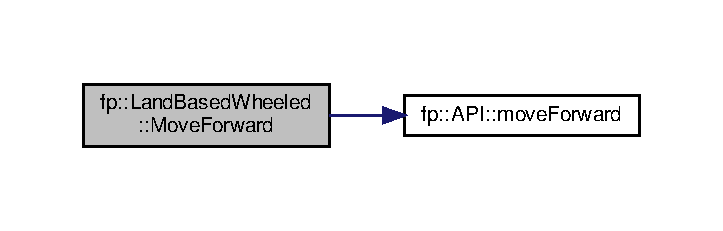
\includegraphics[width=347pt]{classfp_1_1_land_based_wheeled_af7875b805655b6f654e49a885f31122a_cgraph}
\end{center}
\end{figure}
\mbox{\Hypertarget{classfp_1_1_land_based_wheeled_a8fc1115e4c49fec71b38a520df4d1528}\label{classfp_1_1_land_based_wheeled_a8fc1115e4c49fec71b38a520df4d1528}} 
\index{fp\+::\+Land\+Based\+Wheeled@{fp\+::\+Land\+Based\+Wheeled}!Speed\+Up@{Speed\+Up}}
\index{Speed\+Up@{Speed\+Up}!fp\+::\+Land\+Based\+Wheeled@{fp\+::\+Land\+Based\+Wheeled}}
\subsubsection{\texorpdfstring{Speed\+Up()}{SpeedUp()}}
{\footnotesize\ttfamily void fp\+::\+Land\+Based\+Wheeled\+::\+Speed\+Up (\begin{DoxyParamCaption}\item[{int}]{x }\end{DoxyParamCaption})}



This function works for Speed\+Up for wheeled robot. 

This will just ouput that appropriate function are called or not.


\begin{DoxyParams}{Parameters}
{\em int} & \\
\hline
\end{DoxyParams}
\begin{DoxyReturn}{Returns}
none 
\end{DoxyReturn}
\hypertarget{_m_a_z_e_8h_DESCRIPTION}{}\subsection{D\+E\+S\+C\+R\+I\+P\+T\+I\+ON}\label{_m_a_z_e_8h_DESCRIPTION}
F\+U\+N\+C\+T\+I\+ON N\+A\+ME -\/ \hyperlink{classfp_1_1_land_based_wheeled_a8fc1115e4c49fec71b38a520df4d1528}{Speed\+Up()} F\+U\+N\+C\+T\+I\+ON P\+A\+R\+A\+M\+E\+T\+ER T\+Y\+PE -\/ integer R\+E\+T\+U\+RN T\+Y\+PE OF \hyperlink{classfp_1_1_land_based_wheeled_a8fc1115e4c49fec71b38a520df4d1528}{Speed\+Up()} is void.\hypertarget{main_8cpp_Description}{}\subsection{Description}\label{main_8cpp_Description}
F\+U\+N\+C\+T\+I\+ON N\+A\+ME -\/ Speedup F\+U\+N\+C\+T\+I\+ON P\+A\+R\+A\+M\+E\+T\+ER T\+Y\+PE -\/ integer \mbox{\Hypertarget{classfp_1_1_land_based_wheeled_a2f2434db907aaef26b8f3084e84b3579}\label{classfp_1_1_land_based_wheeled_a2f2434db907aaef26b8f3084e84b3579}} 
\index{fp\+::\+Land\+Based\+Wheeled@{fp\+::\+Land\+Based\+Wheeled}!Turn\+Left@{Turn\+Left}}
\index{Turn\+Left@{Turn\+Left}!fp\+::\+Land\+Based\+Wheeled@{fp\+::\+Land\+Based\+Wheeled}}
\subsubsection{\texorpdfstring{Turn\+Left()}{TurnLeft()}}
{\footnotesize\ttfamily void fp\+::\+Land\+Based\+Wheeled\+::\+Turn\+Left (\begin{DoxyParamCaption}\item[{int}]{x,  }\item[{int}]{y }\end{DoxyParamCaption})\hspace{0.3cm}{\ttfamily [override]}, {\ttfamily [virtual]}}



This function works for Turnleft for wheeled robot. 

This will just ouput that appropriate function are called or not.


\begin{DoxyParams}{Parameters}
{\em int} & \\
\hline
{\em int} & \\
\hline
\end{DoxyParams}
\begin{DoxyReturn}{Returns}
none 
\end{DoxyReturn}
\hypertarget{_m_a_z_e_8h_DESCRIPTION}{}\subsection{D\+E\+S\+C\+R\+I\+P\+T\+I\+ON}\label{_m_a_z_e_8h_DESCRIPTION}
F\+U\+N\+C\+T\+I\+ON N\+A\+ME -\/ \hyperlink{classfp_1_1_land_based_wheeled_a2f2434db907aaef26b8f3084e84b3579}{Turn\+Left()} F\+U\+N\+C\+T\+I\+ON P\+A\+R\+A\+M\+E\+T\+ER T\+Y\+PE -\/ integers R\+E\+T\+U\+RN T\+Y\+PE OF \hyperlink{classfp_1_1_land_based_wheeled_a2f2434db907aaef26b8f3084e84b3579}{Turn\+Left()} is void.\hypertarget{main_8cpp_Description}{}\subsection{Description}\label{main_8cpp_Description}
F\+U\+N\+C\+T\+I\+ON N\+A\+ME -\/ Turn\+Left F\+U\+N\+C\+T\+I\+ON P\+A\+R\+A\+M\+E\+T\+ER T\+Y\+PE -\/ two integers 

Implements \hyperlink{classfp_1_1_land_based_robot_a359e1012e9093475b7a1b0d38e41a118}{fp\+::\+Land\+Based\+Robot}.

Here is the call graph for this function\+:
\nopagebreak
\begin{figure}[H]
\begin{center}
\leavevmode
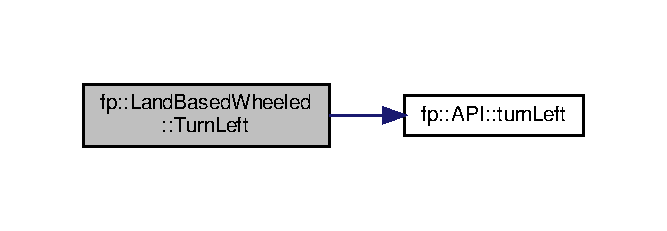
\includegraphics[width=320pt]{classfp_1_1_land_based_wheeled_a2f2434db907aaef26b8f3084e84b3579_cgraph}
\end{center}
\end{figure}
\mbox{\Hypertarget{classfp_1_1_land_based_wheeled_ac6e93b00e624e281a497e99729db04e7}\label{classfp_1_1_land_based_wheeled_ac6e93b00e624e281a497e99729db04e7}} 
\index{fp\+::\+Land\+Based\+Wheeled@{fp\+::\+Land\+Based\+Wheeled}!Turn\+Right@{Turn\+Right}}
\index{Turn\+Right@{Turn\+Right}!fp\+::\+Land\+Based\+Wheeled@{fp\+::\+Land\+Based\+Wheeled}}
\subsubsection{\texorpdfstring{Turn\+Right()}{TurnRight()}}
{\footnotesize\ttfamily void fp\+::\+Land\+Based\+Wheeled\+::\+Turn\+Right (\begin{DoxyParamCaption}\item[{int}]{x,  }\item[{int}]{y }\end{DoxyParamCaption})\hspace{0.3cm}{\ttfamily [override]}, {\ttfamily [virtual]}}



This function works for Turn\+Right for wheeled robot. 

This will just ouput that appropriate function are called or not.


\begin{DoxyParams}{Parameters}
{\em int} & \\
\hline
{\em int} & \\
\hline
\end{DoxyParams}
\begin{DoxyReturn}{Returns}
none 
\end{DoxyReturn}
\hypertarget{_m_a_z_e_8h_DESCRIPTION}{}\subsection{D\+E\+S\+C\+R\+I\+P\+T\+I\+ON}\label{_m_a_z_e_8h_DESCRIPTION}
F\+U\+N\+C\+T\+I\+ON N\+A\+ME -\/ \hyperlink{classfp_1_1_land_based_wheeled_ac6e93b00e624e281a497e99729db04e7}{Turn\+Right()} F\+U\+N\+C\+T\+I\+ON P\+A\+R\+A\+M\+E\+T\+ER T\+Y\+PE -\/ integers R\+E\+T\+U\+RN T\+Y\+PE OF \hyperlink{classfp_1_1_land_based_wheeled_ac6e93b00e624e281a497e99729db04e7}{Turn\+Right()} is void.\hypertarget{main_8cpp_Description}{}\subsection{Description}\label{main_8cpp_Description}
F\+U\+N\+C\+T\+I\+ON N\+A\+ME -\/ Turn\+Right F\+U\+N\+C\+T\+I\+ON P\+A\+R\+A\+M\+E\+T\+ER T\+Y\+PE -\/ two integers 

Implements \hyperlink{classfp_1_1_land_based_robot_a7360e4084bc5254f72ab0d3612644907}{fp\+::\+Land\+Based\+Robot}.

Here is the call graph for this function\+:
\nopagebreak
\begin{figure}[H]
\begin{center}
\leavevmode
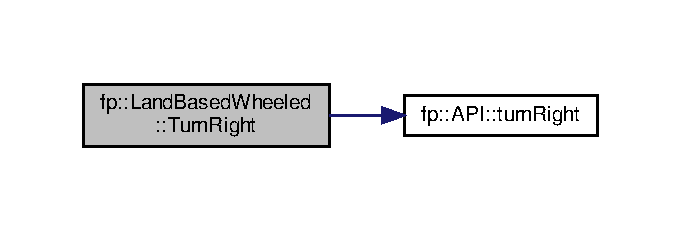
\includegraphics[width=327pt]{classfp_1_1_land_based_wheeled_ac6e93b00e624e281a497e99729db04e7_cgraph}
\end{center}
\end{figure}


\subsection{Member Data Documentation}
\mbox{\Hypertarget{classfp_1_1_land_based_wheeled_ac50206eb412222a4d3c8f494c5dbd09b}\label{classfp_1_1_land_based_wheeled_ac50206eb412222a4d3c8f494c5dbd09b}} 
\index{fp\+::\+Land\+Based\+Wheeled@{fp\+::\+Land\+Based\+Wheeled}!wheel\+\_\+number@{wheel\+\_\+number}}
\index{wheel\+\_\+number@{wheel\+\_\+number}!fp\+::\+Land\+Based\+Wheeled@{fp\+::\+Land\+Based\+Wheeled}}
\subsubsection{\texorpdfstring{wheel\+\_\+number}{wheel\_number}}
{\footnotesize\ttfamily int fp\+::\+Land\+Based\+Wheeled\+::wheel\+\_\+number\hspace{0.3cm}{\ttfamily [protected]}}



The documentation for this class was generated from the following files\+:\begin{DoxyCompactItemize}
\item 
src/\+Land\+Based\+Wheeled/\hyperlink{_land_based_wheeled_8h}{Land\+Based\+Wheeled.\+h}\item 
src/\+Land\+Based\+Wheeled/\hyperlink{_land_based_wheeled_8cpp}{Land\+Based\+Wheeled.\+cpp}\end{DoxyCompactItemize}

\hypertarget{classfp_1_1_maze}{}\section{fp\+:\+:Maze Class Reference}
\label{classfp_1_1_maze}\index{fp\+::\+Maze@{fp\+::\+Maze}}


{\ttfamily \#include $<$M\+A\+Z\+E.\+h$>$}

\subsection*{Public Member Functions}
\begin{DoxyCompactItemize}
\item 
\hyperlink{classfp_1_1_maze_af090b97595ed34cad9f7c8de9e79a127}{Maze} ()
\begin{DoxyCompactList}\small\item\em A constructor. \end{DoxyCompactList}\item 
void \hyperlink{classfp_1_1_maze_a9771da7e8af1d23454f9b5cb1986462b}{Maze\+Design} (int x, int y, char dir)
\begin{DoxyCompactList}\small\item\em this is for the design of the a maze based on the co-\/ordinates given here in x,y parameter. \end{DoxyCompactList}\item 
void \hyperlink{classfp_1_1_maze_a7aed0c5288e08efda078782f23bc8368}{Maze\+Construct} ()
\item 
bool \hyperlink{classfp_1_1_maze_a6cc110e308818595983345285245c33f}{South\+Wall\+Present} (int x, int y) const
\begin{DoxyCompactList}\small\item\em to check at specific location in maze is wall or space in south direction. \end{DoxyCompactList}\item 
bool \hyperlink{classfp_1_1_maze_af072147db014d3955ba343cd8250d5f1}{North\+Wall\+Present} (int x, int y) const
\begin{DoxyCompactList}\small\item\em to check at specific location in maze is wall or space in north direction. \end{DoxyCompactList}\item 
bool \hyperlink{classfp_1_1_maze_a62c5692927ef95bafad2f0b7ae95a83e}{West\+Wall\+Present} (int x, int y) const
\begin{DoxyCompactList}\small\item\em to check at specific location in maze is wall or space in west direction. \end{DoxyCompactList}\item 
bool \hyperlink{classfp_1_1_maze_aed00bd0afedc44d52c1949dd769e68c2}{East\+Wall\+Present} (int x, int y) const
\begin{DoxyCompactList}\small\item\em function is called wether the wall is present in the east direction \end{DoxyCompactList}\item 
\hyperlink{classfp_1_1_maze_ae5f5b10dd66d6a994a40da62fef39577}{$\sim$\+Maze} ()
\begin{DoxyCompactList}\small\item\em to check at specific location in maze is wall or space in east direction. \end{DoxyCompactList}\end{DoxyCompactItemize}
\subsection*{Protected Attributes}
\begin{DoxyCompactItemize}
\item 
int \hyperlink{classfp_1_1_maze_a856f8a1002fdad16684454cb6006646a}{Wall\+DetectedS} \mbox{[}16\mbox{]}\mbox{[}16\mbox{]}
\item 
int \hyperlink{classfp_1_1_maze_aa3538c38fcd8c6cddf3046ec3a33ab2e}{Wall\+DetectedN} \mbox{[}16\mbox{]}\mbox{[}16\mbox{]}
\item 
int \hyperlink{classfp_1_1_maze_ad93e8c8272e3b2f9f693238a95dc38c1}{Wall\+DetectedW} \mbox{[}16\mbox{]}\mbox{[}16\mbox{]}
\item 
int \hyperlink{classfp_1_1_maze_aaa20ddff203607af6ee3c95a00e2d2bf}{Wall\+DetectedE} \mbox{[}16\mbox{]}\mbox{[}16\mbox{]}
\end{DoxyCompactItemize}


\subsection{Detailed Description}
\begin{DoxyAuthor}{Author}
Group-\/9 E\+N\+P\+M809Y 
\end{DoxyAuthor}
\begin{DoxyDate}{Date}
03/12/19 
\end{DoxyDate}


\subsection{Constructor \& Destructor Documentation}
\mbox{\Hypertarget{classfp_1_1_maze_af090b97595ed34cad9f7c8de9e79a127}\label{classfp_1_1_maze_af090b97595ed34cad9f7c8de9e79a127}} 
\index{fp\+::\+Maze@{fp\+::\+Maze}!Maze@{Maze}}
\index{Maze@{Maze}!fp\+::\+Maze@{fp\+::\+Maze}}
\subsubsection{\texorpdfstring{Maze()}{Maze()}}
{\footnotesize\ttfamily fp\+::\+Maze\+::\+Maze (\begin{DoxyParamCaption}{ }\end{DoxyParamCaption})}



A constructor. 

This is declareation for class maze which are wrapped up in the fp namespace.

A constructor that takes no arguments.\hypertarget{_m_a_z_e_8h_DESCRIPTION}{}\subsection{D\+E\+S\+C\+R\+I\+P\+T\+I\+ON}\label{_m_a_z_e_8h_DESCRIPTION}
We have derived a lot of functions from the api file like set colors and set\+\_\+text in the maze file. Basically from the derived api untill we meet the wall we craete the maze here. Here is the call graph for this function\+:
\nopagebreak
\begin{figure}[H]
\begin{center}
\leavevmode
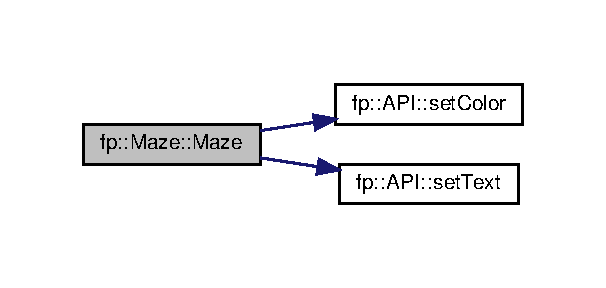
\includegraphics[width=291pt]{classfp_1_1_maze_af090b97595ed34cad9f7c8de9e79a127_cgraph}
\end{center}
\end{figure}
\mbox{\Hypertarget{classfp_1_1_maze_ae5f5b10dd66d6a994a40da62fef39577}\label{classfp_1_1_maze_ae5f5b10dd66d6a994a40da62fef39577}} 
\index{fp\+::\+Maze@{fp\+::\+Maze}!````~Maze@{$\sim$\+Maze}}
\index{````~Maze@{$\sim$\+Maze}!fp\+::\+Maze@{fp\+::\+Maze}}
\subsubsection{\texorpdfstring{$\sim$\+Maze()}{~Maze()}}
{\footnotesize\ttfamily fp\+::\+Maze\+::$\sim$\+Maze (\begin{DoxyParamCaption}{ }\end{DoxyParamCaption})\hspace{0.3cm}{\ttfamily [inline]}}



to check at specific location in maze is wall or space in east direction. 


\begin{DoxyParams}{Parameters}
{\em x} & \\
\hline
{\em y} & \\
\hline
\end{DoxyParams}
\begin{DoxyReturn}{Returns}
intA destructor 
\end{DoxyReturn}


\subsection{Member Function Documentation}
\mbox{\Hypertarget{classfp_1_1_maze_aed00bd0afedc44d52c1949dd769e68c2}\label{classfp_1_1_maze_aed00bd0afedc44d52c1949dd769e68c2}} 
\index{fp\+::\+Maze@{fp\+::\+Maze}!East\+Wall\+Present@{East\+Wall\+Present}}
\index{East\+Wall\+Present@{East\+Wall\+Present}!fp\+::\+Maze@{fp\+::\+Maze}}
\subsubsection{\texorpdfstring{East\+Wall\+Present()}{EastWallPresent()}}
{\footnotesize\ttfamily bool fp\+::\+Maze\+::\+East\+Wall\+Present (\begin{DoxyParamCaption}\item[{int}]{x,  }\item[{int}]{y }\end{DoxyParamCaption}) const}



function is called wether the wall is present in the east direction 


\begin{DoxyParams}{Parameters}
{\em x} & \\
\hline
{\em y} & \\
\hline
\end{DoxyParams}
\begin{DoxyReturn}{Returns}
true/false based on the api function Wall\+Detected. 
\end{DoxyReturn}
Here is the caller graph for this function\+:
\nopagebreak
\begin{figure}[H]
\begin{center}
\leavevmode
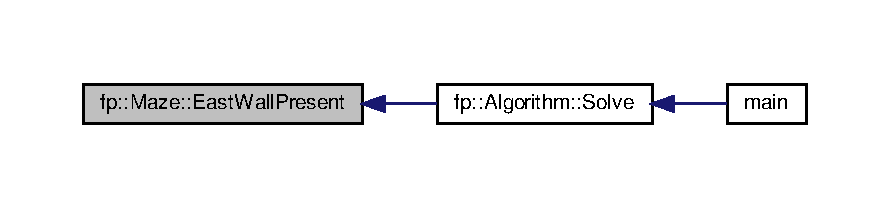
\includegraphics[width=350pt]{classfp_1_1_maze_aed00bd0afedc44d52c1949dd769e68c2_icgraph}
\end{center}
\end{figure}
\mbox{\Hypertarget{classfp_1_1_maze_a7aed0c5288e08efda078782f23bc8368}\label{classfp_1_1_maze_a7aed0c5288e08efda078782f23bc8368}} 
\index{fp\+::\+Maze@{fp\+::\+Maze}!Maze\+Construct@{Maze\+Construct}}
\index{Maze\+Construct@{Maze\+Construct}!fp\+::\+Maze@{fp\+::\+Maze}}
\subsubsection{\texorpdfstring{Maze\+Construct()}{MazeConstruct()}}
{\footnotesize\ttfamily void fp\+::\+Maze\+::\+Maze\+Construct (\begin{DoxyParamCaption}{ }\end{DoxyParamCaption})}

\mbox{\Hypertarget{classfp_1_1_maze_a9771da7e8af1d23454f9b5cb1986462b}\label{classfp_1_1_maze_a9771da7e8af1d23454f9b5cb1986462b}} 
\index{fp\+::\+Maze@{fp\+::\+Maze}!Maze\+Design@{Maze\+Design}}
\index{Maze\+Design@{Maze\+Design}!fp\+::\+Maze@{fp\+::\+Maze}}
\subsubsection{\texorpdfstring{Maze\+Design()}{MazeDesign()}}
{\footnotesize\ttfamily void fp\+::\+Maze\+::\+Maze\+Design (\begin{DoxyParamCaption}\item[{int}]{x,  }\item[{int}]{y,  }\item[{char}]{dir }\end{DoxyParamCaption})}



this is for the design of the a maze based on the co-\/ordinates given here in x,y parameter. 

this is for the design of the amze based on the co-\/ordinates given here in x,y parameter.


\begin{DoxyParams}{Parameters}
{\em x-\/} & x co-\/ordinate \\
\hline
{\em y} & -\/y co-\/ordinate \\
\hline
{\em dir} & a char to set up direction from N,E,W,S \\
\hline
\end{DoxyParams}
\hypertarget{_m_a_z_e_8h_DESCRIPTION}{}\subsection{D\+E\+S\+C\+R\+I\+P\+T\+I\+ON}\label{_m_a_z_e_8h_DESCRIPTION}
A very simple wrapped function(in fp namespace to construct a maze which will with given co-\/ordinates desihn a maze and detailed explanation is in implementation file.


\begin{DoxyParams}{Parameters}
{\em x-\/} & x co-\/ordinate \\
\hline
{\em y} & -\/y co-\/ordinate \\
\hline
{\em dir} & a char to set up direction from N,E,W,S \\
\hline
\end{DoxyParams}
\hypertarget{_m_a_z_e_8h_DESCRIPTION}{}\subsection{D\+E\+S\+C\+R\+I\+P\+T\+I\+ON}\label{_m_a_z_e_8h_DESCRIPTION}
A very simple wrapped function(in fp namespace in header file) to design a maze Here for each direction we check for the wallchoice and if the from the api header file we are not meeting to wall we are good to go and it writes a maze and that is why we have 4 different condition for 4 different directions for each option(\+N,\+S,\+E,\+W). and if we met true than we write it in maze. Here is the call graph for this function\+:
\nopagebreak
\begin{figure}[H]
\begin{center}
\leavevmode
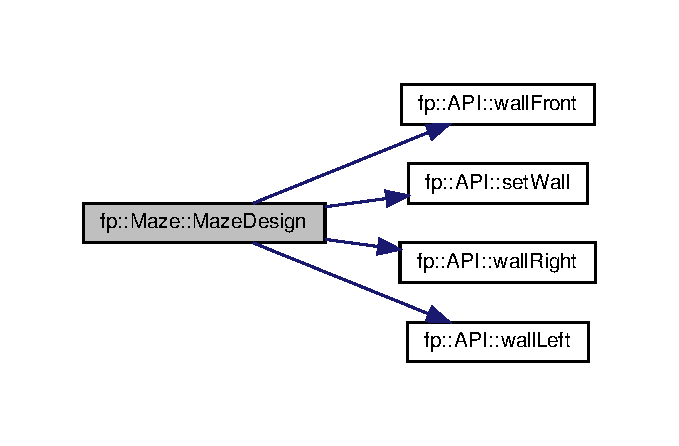
\includegraphics[width=326pt]{classfp_1_1_maze_a9771da7e8af1d23454f9b5cb1986462b_cgraph}
\end{center}
\end{figure}
Here is the caller graph for this function\+:
\nopagebreak
\begin{figure}[H]
\begin{center}
\leavevmode
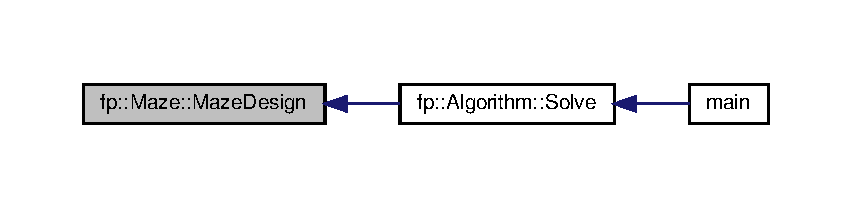
\includegraphics[width=350pt]{classfp_1_1_maze_a9771da7e8af1d23454f9b5cb1986462b_icgraph}
\end{center}
\end{figure}
\mbox{\Hypertarget{classfp_1_1_maze_af072147db014d3955ba343cd8250d5f1}\label{classfp_1_1_maze_af072147db014d3955ba343cd8250d5f1}} 
\index{fp\+::\+Maze@{fp\+::\+Maze}!North\+Wall\+Present@{North\+Wall\+Present}}
\index{North\+Wall\+Present@{North\+Wall\+Present}!fp\+::\+Maze@{fp\+::\+Maze}}
\subsubsection{\texorpdfstring{North\+Wall\+Present()}{NorthWallPresent()}}
{\footnotesize\ttfamily bool fp\+::\+Maze\+::\+North\+Wall\+Present (\begin{DoxyParamCaption}\item[{int}]{x,  }\item[{int}]{y }\end{DoxyParamCaption}) const}



to check at specific location in maze is wall or space in north direction. 

function is called wether the wall is present in the north direction.


\begin{DoxyParams}{Parameters}
{\em x} & \\
\hline
{\em y} & \\
\hline
\end{DoxyParams}
\begin{DoxyReturn}{Returns}
int
\end{DoxyReturn}

\begin{DoxyParams}{Parameters}
{\em x} & \\
\hline
{\em y} & \\
\hline
\end{DoxyParams}
\begin{DoxyReturn}{Returns}
true/false based on the api function Wall\+Detected. 
\end{DoxyReturn}
Here is the caller graph for this function\+:
\nopagebreak
\begin{figure}[H]
\begin{center}
\leavevmode
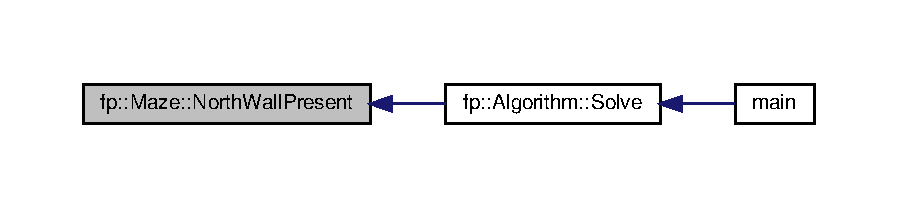
\includegraphics[width=350pt]{classfp_1_1_maze_af072147db014d3955ba343cd8250d5f1_icgraph}
\end{center}
\end{figure}
\mbox{\Hypertarget{classfp_1_1_maze_a6cc110e308818595983345285245c33f}\label{classfp_1_1_maze_a6cc110e308818595983345285245c33f}} 
\index{fp\+::\+Maze@{fp\+::\+Maze}!South\+Wall\+Present@{South\+Wall\+Present}}
\index{South\+Wall\+Present@{South\+Wall\+Present}!fp\+::\+Maze@{fp\+::\+Maze}}
\subsubsection{\texorpdfstring{South\+Wall\+Present()}{SouthWallPresent()}}
{\footnotesize\ttfamily bool fp\+::\+Maze\+::\+South\+Wall\+Present (\begin{DoxyParamCaption}\item[{int}]{x,  }\item[{int}]{y }\end{DoxyParamCaption}) const}



to check at specific location in maze is wall or space in south direction. 

function is called wether the wall is present in the south direction


\begin{DoxyParams}{Parameters}
{\em x} & \\
\hline
{\em y} & \\
\hline
\end{DoxyParams}
\begin{DoxyReturn}{Returns}
int
\end{DoxyReturn}

\begin{DoxyParams}{Parameters}
{\em x} & \\
\hline
{\em y} & \\
\hline
\end{DoxyParams}
\begin{DoxyReturn}{Returns}
true/false based on the api function Wall\+Detected. 
\end{DoxyReturn}
Here is the caller graph for this function\+:
\nopagebreak
\begin{figure}[H]
\begin{center}
\leavevmode
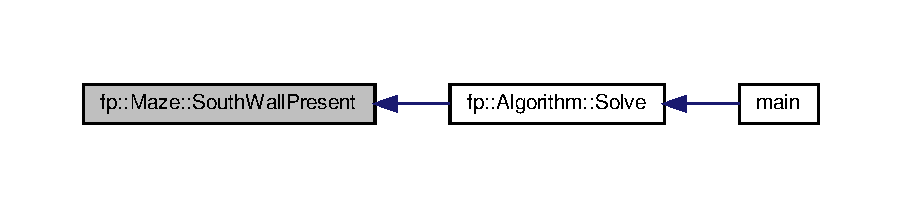
\includegraphics[width=350pt]{classfp_1_1_maze_a6cc110e308818595983345285245c33f_icgraph}
\end{center}
\end{figure}
\mbox{\Hypertarget{classfp_1_1_maze_a62c5692927ef95bafad2f0b7ae95a83e}\label{classfp_1_1_maze_a62c5692927ef95bafad2f0b7ae95a83e}} 
\index{fp\+::\+Maze@{fp\+::\+Maze}!West\+Wall\+Present@{West\+Wall\+Present}}
\index{West\+Wall\+Present@{West\+Wall\+Present}!fp\+::\+Maze@{fp\+::\+Maze}}
\subsubsection{\texorpdfstring{West\+Wall\+Present()}{WestWallPresent()}}
{\footnotesize\ttfamily bool fp\+::\+Maze\+::\+West\+Wall\+Present (\begin{DoxyParamCaption}\item[{int}]{x,  }\item[{int}]{y }\end{DoxyParamCaption}) const}



to check at specific location in maze is wall or space in west direction. 

function is called wether the wall is present in the west direction


\begin{DoxyParams}{Parameters}
{\em x} & \\
\hline
{\em y} & \\
\hline
\end{DoxyParams}
\begin{DoxyReturn}{Returns}
int
\end{DoxyReturn}

\begin{DoxyParams}{Parameters}
{\em x} & \\
\hline
{\em y} & \\
\hline
\end{DoxyParams}
\begin{DoxyReturn}{Returns}
true/false based on the api function Wall\+Detected. 
\end{DoxyReturn}
Here is the caller graph for this function\+:
\nopagebreak
\begin{figure}[H]
\begin{center}
\leavevmode
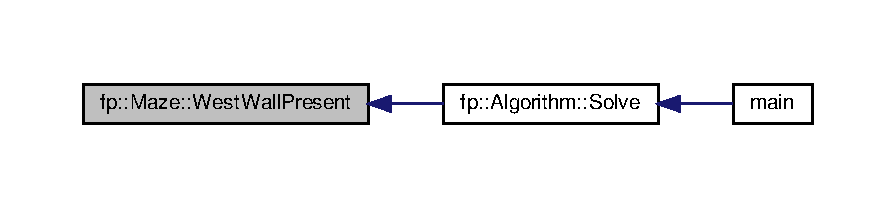
\includegraphics[width=350pt]{classfp_1_1_maze_a62c5692927ef95bafad2f0b7ae95a83e_icgraph}
\end{center}
\end{figure}


\subsection{Member Data Documentation}
\mbox{\Hypertarget{classfp_1_1_maze_aaa20ddff203607af6ee3c95a00e2d2bf}\label{classfp_1_1_maze_aaa20ddff203607af6ee3c95a00e2d2bf}} 
\index{fp\+::\+Maze@{fp\+::\+Maze}!Wall\+DetectedE@{Wall\+DetectedE}}
\index{Wall\+DetectedE@{Wall\+DetectedE}!fp\+::\+Maze@{fp\+::\+Maze}}
\subsubsection{\texorpdfstring{Wall\+DetectedE}{WallDetectedE}}
{\footnotesize\ttfamily int fp\+::\+Maze\+::\+Wall\+DetectedE\mbox{[}16\mbox{]}\mbox{[}16\mbox{]}\hspace{0.3cm}{\ttfamily [protected]}}

a matrix to check wether wall detected in east direction \mbox{\Hypertarget{classfp_1_1_maze_aa3538c38fcd8c6cddf3046ec3a33ab2e}\label{classfp_1_1_maze_aa3538c38fcd8c6cddf3046ec3a33ab2e}} 
\index{fp\+::\+Maze@{fp\+::\+Maze}!Wall\+DetectedN@{Wall\+DetectedN}}
\index{Wall\+DetectedN@{Wall\+DetectedN}!fp\+::\+Maze@{fp\+::\+Maze}}
\subsubsection{\texorpdfstring{Wall\+DetectedN}{WallDetectedN}}
{\footnotesize\ttfamily int fp\+::\+Maze\+::\+Wall\+DetectedN\mbox{[}16\mbox{]}\mbox{[}16\mbox{]}\hspace{0.3cm}{\ttfamily [protected]}}

a matrix to check wether wall detected in north direction \mbox{\Hypertarget{classfp_1_1_maze_a856f8a1002fdad16684454cb6006646a}\label{classfp_1_1_maze_a856f8a1002fdad16684454cb6006646a}} 
\index{fp\+::\+Maze@{fp\+::\+Maze}!Wall\+DetectedS@{Wall\+DetectedS}}
\index{Wall\+DetectedS@{Wall\+DetectedS}!fp\+::\+Maze@{fp\+::\+Maze}}
\subsubsection{\texorpdfstring{Wall\+DetectedS}{WallDetectedS}}
{\footnotesize\ttfamily int fp\+::\+Maze\+::\+Wall\+DetectedS\mbox{[}16\mbox{]}\mbox{[}16\mbox{]}\hspace{0.3cm}{\ttfamily [protected]}}

a matrix to check wether wall detected in south direction \mbox{\Hypertarget{classfp_1_1_maze_ad93e8c8272e3b2f9f693238a95dc38c1}\label{classfp_1_1_maze_ad93e8c8272e3b2f9f693238a95dc38c1}} 
\index{fp\+::\+Maze@{fp\+::\+Maze}!Wall\+DetectedW@{Wall\+DetectedW}}
\index{Wall\+DetectedW@{Wall\+DetectedW}!fp\+::\+Maze@{fp\+::\+Maze}}
\subsubsection{\texorpdfstring{Wall\+DetectedW}{WallDetectedW}}
{\footnotesize\ttfamily int fp\+::\+Maze\+::\+Wall\+DetectedW\mbox{[}16\mbox{]}\mbox{[}16\mbox{]}\hspace{0.3cm}{\ttfamily [protected]}}

a matrix to check wether wall detected in west direction 

The documentation for this class was generated from the following files\+:\begin{DoxyCompactItemize}
\item 
src/\+Maze/\hyperlink{_m_a_z_e_8h}{M\+A\+Z\+E.\+h}\item 
src/\+Maze/\hyperlink{_m_a_z_e_8cpp}{M\+A\+Z\+E.\+cpp}\end{DoxyCompactItemize}

\chapter{File Documentation}
\hypertarget{main_8cpp}{}\section{main.\+cpp File Reference}
\label{main_8cpp}\index{main.\+cpp@{main.\+cpp}}
{\ttfamily \#include \char`\"{}src/\+Land\+Based\+Wheeled/\+Land\+Based\+Wheeled.\+h\char`\"{}}\newline
{\ttfamily \#include \char`\"{}src/\+Land\+Based\+Tracked/\+Land\+Based\+Tracked.\+h\char`\"{}}\newline
{\ttfamily \#include \char`\"{}src/\+Land\+Based\+Robot/\+Land\+Based\+Robot.\+h\char`\"{}}\newline
{\ttfamily \#include \char`\"{}src/\+Algorithm/\+Algorithm.\+h\char`\"{}}\newline
{\ttfamily \#include \char`\"{}src/\+Maze/\+M\+A\+Z\+E.\+h\char`\"{}}\newline
{\ttfamily \#include $<$vector$>$}\newline
{\ttfamily \#include $<$iostream$>$}\newline
Include dependency graph for main.\+cpp\+:
\nopagebreak
\begin{figure}[H]
\begin{center}
\leavevmode
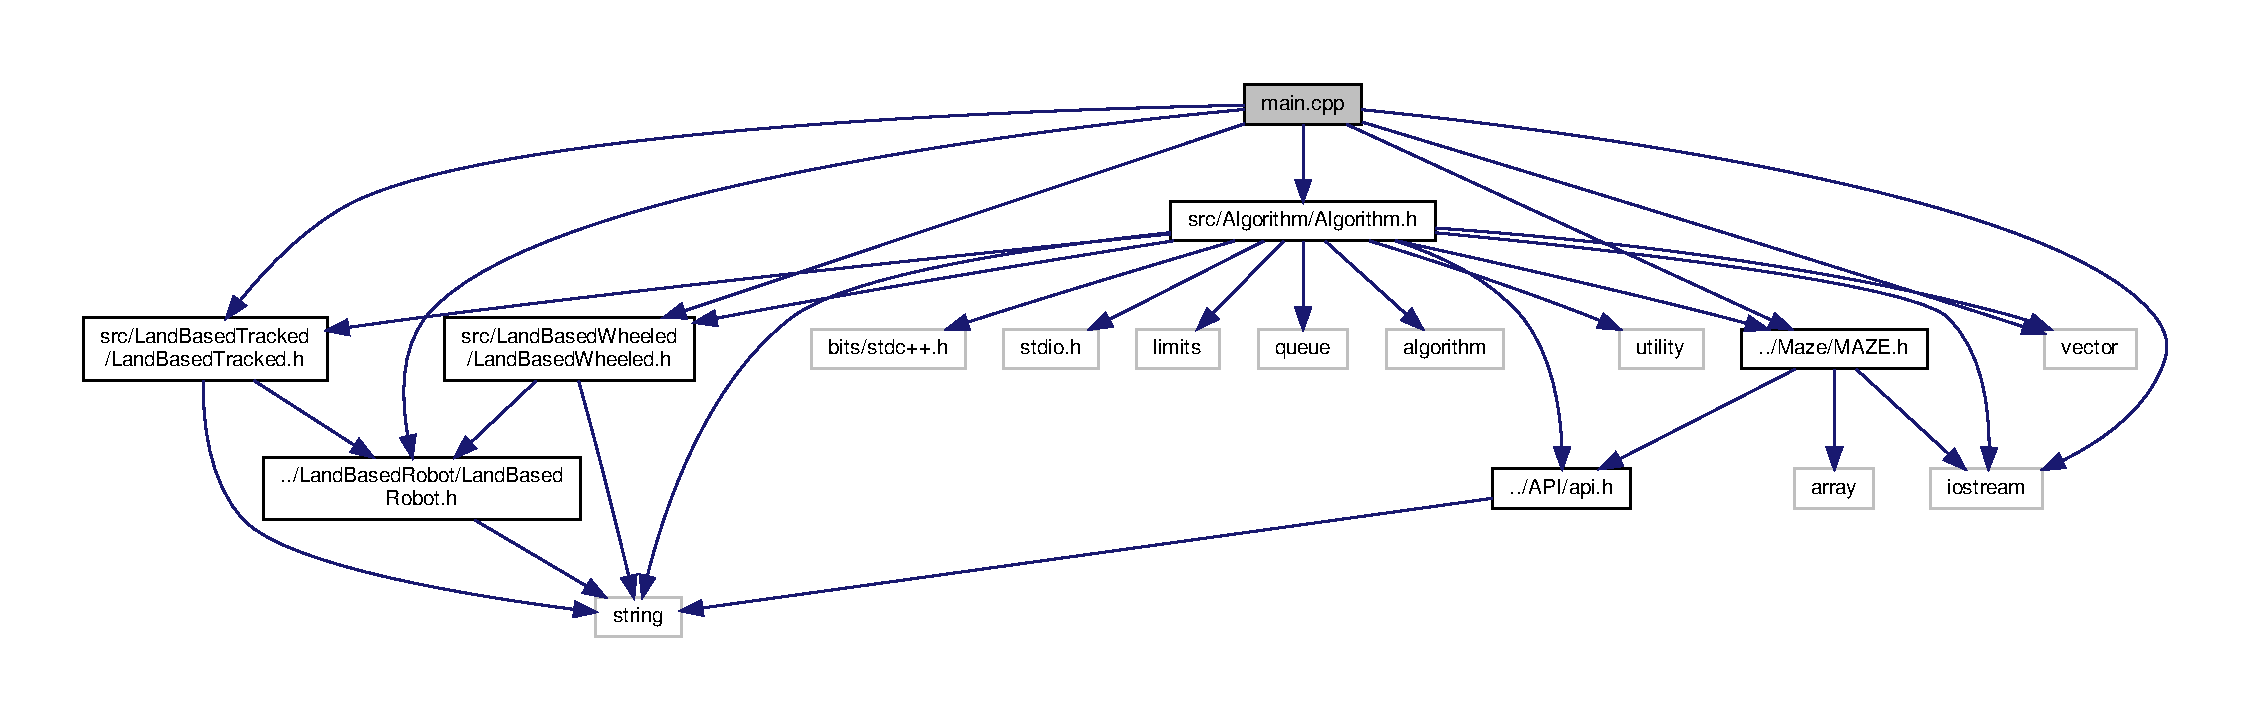
\includegraphics[width=350pt]{main_8cpp__incl}
\end{center}
\end{figure}
\subsection*{Functions}
\begin{DoxyCompactItemize}
\item 
void \hyperlink{main_8cpp_ae8eeaa075074957bc51d38efe1d1868b}{Follow\+Action\+Path} (\hyperlink{classfp_1_1_land_based_robot}{fp\+::\+Land\+Based\+Robot} $\ast$robot, const std\+::vector$<$ std\+::string $>$ \&vec, std\+::string obj)
\item 
int \hyperlink{main_8cpp_ae66f6b31b5ad750f1fe042a706a4e3d4}{main} ()
\begin{DoxyCompactList}\small\item\em Main function. \end{DoxyCompactList}\end{DoxyCompactItemize}


\subsection{Detailed Description}
\begin{DoxyAuthor}{Author}
Group9 $<$\+E\+N\+P\+M809\+Y$>$ 
\end{DoxyAuthor}
\begin{DoxyVersion}{Version}
2.\+0
\end{DoxyVersion}
\hypertarget{_m_a_z_e_8h_LICENSE}{}\subsection{L\+I\+C\+E\+N\+SE}\label{_m_a_z_e_8h_LICENSE}
This program is free software; you can redistribute it and/or modify it under the terms of the G\+NU General Public License as published by the Free Software Foundation; either version 2 of the License, or (at your option) any later version.\hypertarget{_m_a_z_e_8h_DESCRIPTION}{}\subsection{D\+E\+S\+C\+R\+I\+P\+T\+I\+ON}\label{_m_a_z_e_8h_DESCRIPTION}
This C++ program is kind of a test file where prototyped definitions of class can take solid action. So here have included all the header files which basically contains functions for the \hyperlink{main_8cpp}{main.\+cpp} to work. 

\subsection{Function Documentation}
\mbox{\Hypertarget{main_8cpp_ae8eeaa075074957bc51d38efe1d1868b}\label{main_8cpp_ae8eeaa075074957bc51d38efe1d1868b}} 
\index{main.\+cpp@{main.\+cpp}!Follow\+Action\+Path@{Follow\+Action\+Path}}
\index{Follow\+Action\+Path@{Follow\+Action\+Path}!main.\+cpp@{main.\+cpp}}
\subsubsection{\texorpdfstring{Follow\+Action\+Path()}{FollowActionPath()}}
{\footnotesize\ttfamily void Follow\+Action\+Path (\begin{DoxyParamCaption}\item[{\hyperlink{classfp_1_1_land_based_robot}{fp\+::\+Land\+Based\+Robot} $\ast$}]{robot,  }\item[{const std\+::vector$<$ std\+::string $>$ \&}]{vec,  }\item[{std\+::string}]{obj }\end{DoxyParamCaption})}

Here is the call graph for this function\+:
\nopagebreak
\begin{figure}[H]
\begin{center}
\leavevmode
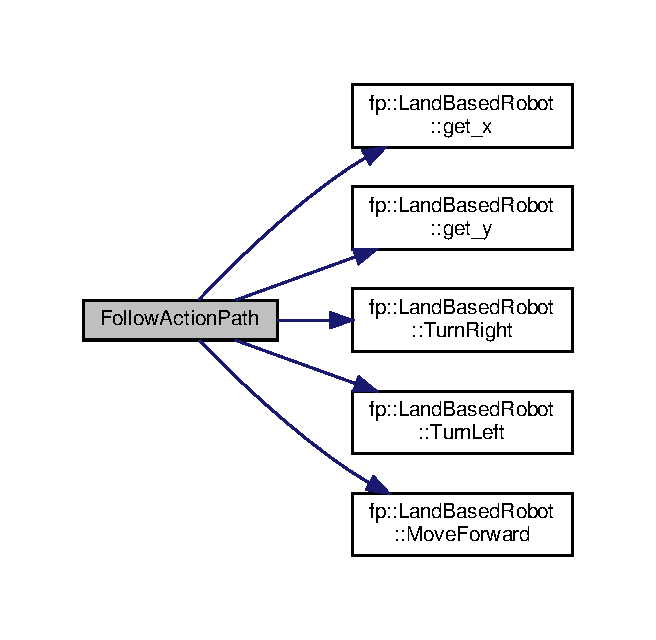
\includegraphics[width=315pt]{main_8cpp_ae8eeaa075074957bc51d38efe1d1868b_cgraph}
\end{center}
\end{figure}
\mbox{\Hypertarget{main_8cpp_ae66f6b31b5ad750f1fe042a706a4e3d4}\label{main_8cpp_ae66f6b31b5ad750f1fe042a706a4e3d4}} 
\index{main.\+cpp@{main.\+cpp}!main@{main}}
\index{main@{main}!main.\+cpp@{main.\+cpp}}
\subsubsection{\texorpdfstring{main()}{main()}}
{\footnotesize\ttfamily int main (\begin{DoxyParamCaption}{ }\end{DoxyParamCaption})}



Main function. 


\begin{DoxyParams}{Parameters}
{\em No} & arguments \\
\hline
{\em No} & Arguments \\
\hline
\end{DoxyParams}
\begin{DoxyReturn}{Returns}
0 
\end{DoxyReturn}
\hypertarget{main_8cpp_Description}{}\subsection{Description}\label{main_8cpp_Description}
The purpose of this method is currently to test whether all classes of this program are being included and implemented. The header files contains the definitions and prototypes whereas the .cpp files contains the implementations of the functions. Land\+Based\+Robot is the base class from which Land\+Basedtracked and Land\+Based\+Wheeled are derived a spart of inheritance. Heirarchical Inheritance is followed where our two classes are derived from one base class. The derived classes inherits the properties, attributes and functions of the base class. Here is the call graph for this function\+:
\nopagebreak
\begin{figure}[H]
\begin{center}
\leavevmode
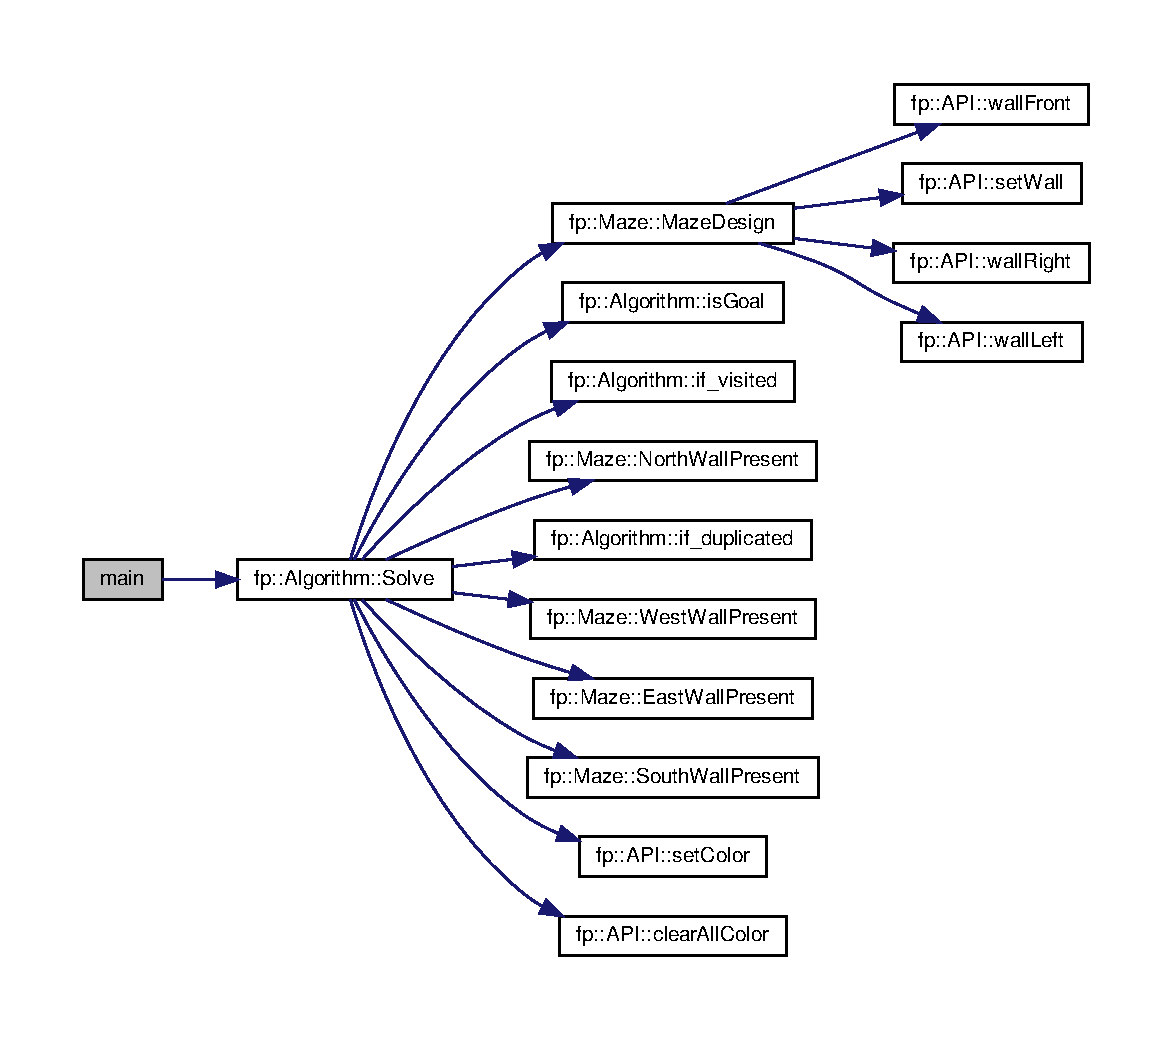
\includegraphics[width=350pt]{main_8cpp_ae66f6b31b5ad750f1fe042a706a4e3d4_cgraph}
\end{center}
\end{figure}

\hypertarget{_algorithm_8cpp}{}\section{src/\+Algorithm/\+Algorithm.cpp File Reference}
\label{_algorithm_8cpp}\index{src/\+Algorithm/\+Algorithm.\+cpp@{src/\+Algorithm/\+Algorithm.\+cpp}}
{\ttfamily \#include \char`\"{}Algorithm.\+h\char`\"{}}\newline
Include dependency graph for Algorithm.\+cpp\+:
\nopagebreak
\begin{figure}[H]
\begin{center}
\leavevmode
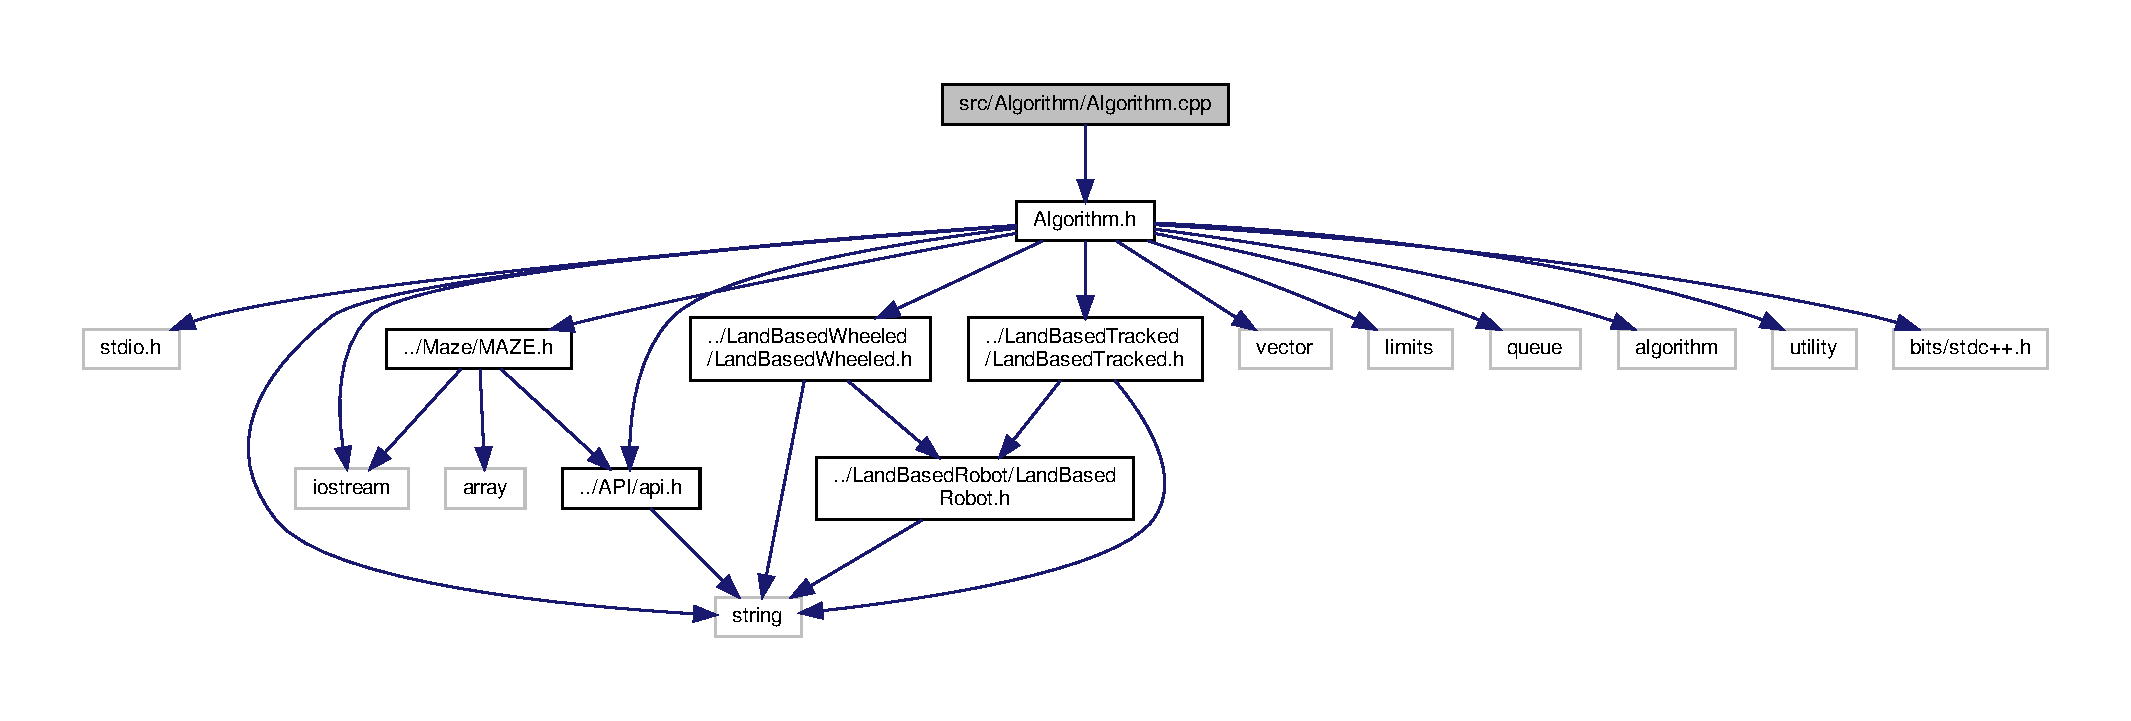
\includegraphics[width=350pt]{_algorithm_8cpp__incl}
\end{center}
\end{figure}


\subsection{Detailed Description}
\begin{DoxyAuthor}{Author}
Group9 $<$\+E\+N\+P\+M809\+Y$>$ 
\end{DoxyAuthor}
\begin{DoxyVersion}{Version}
2.\+0
\end{DoxyVersion}
\hypertarget{_m_a_z_e_8h_LICENSE}{}\subsection{L\+I\+C\+E\+N\+SE}\label{_m_a_z_e_8h_LICENSE}
This program is free software; you can redistribute it and/or modify it under the terms of the G\+NU General Public License as published by the Free Software Foundation; either version 2 of the License, or (at your option) any later version.\hypertarget{_m_a_z_e_8h_DESCRIPTION}{}\subsection{D\+E\+S\+C\+R\+I\+P\+T\+I\+ON}\label{_m_a_z_e_8h_DESCRIPTION}
This C++ program is algorithm implementation for the maze. Applied algorithm is B\+F\+S(\+Brute(\+Breadth) Force Search). All the functions are declared in the \hyperlink{_algorithm_8h}{algorithm.\+h} header file and other library have been included in header files. 
\hypertarget{_algorithm_8h}{}\section{src/\+Algorithm/\+Algorithm.h File Reference}
\label{_algorithm_8h}\index{src/\+Algorithm/\+Algorithm.\+h@{src/\+Algorithm/\+Algorithm.\+h}}


Class to be used in source file and the functions that have been used.  


{\ttfamily \#include $<$stdio.\+h$>$}\newline
{\ttfamily \#include $<$iostream$>$}\newline
{\ttfamily \#include $<$vector$>$}\newline
{\ttfamily \#include $<$string$>$}\newline
{\ttfamily \#include $<$limits$>$}\newline
{\ttfamily \#include $<$queue$>$}\newline
{\ttfamily \#include $<$algorithm$>$}\newline
{\ttfamily \#include $<$utility$>$}\newline
{\ttfamily \#include $<$bits/stdc++.\+h$>$}\newline
{\ttfamily \#include \char`\"{}../\+A\+P\+I/api.\+h\char`\"{}}\newline
{\ttfamily \#include \char`\"{}../\+Land\+Based\+Wheeled/\+Land\+Based\+Wheeled.\+h\char`\"{}}\newline
{\ttfamily \#include \char`\"{}../\+Land\+Based\+Tracked/\+Land\+Based\+Tracked.\+h\char`\"{}}\newline
{\ttfamily \#include \char`\"{}../\+Maze/\+M\+A\+Z\+E.\+h\char`\"{}}\newline
Include dependency graph for Algorithm.\+h\+:
\nopagebreak
\begin{figure}[H]
\begin{center}
\leavevmode
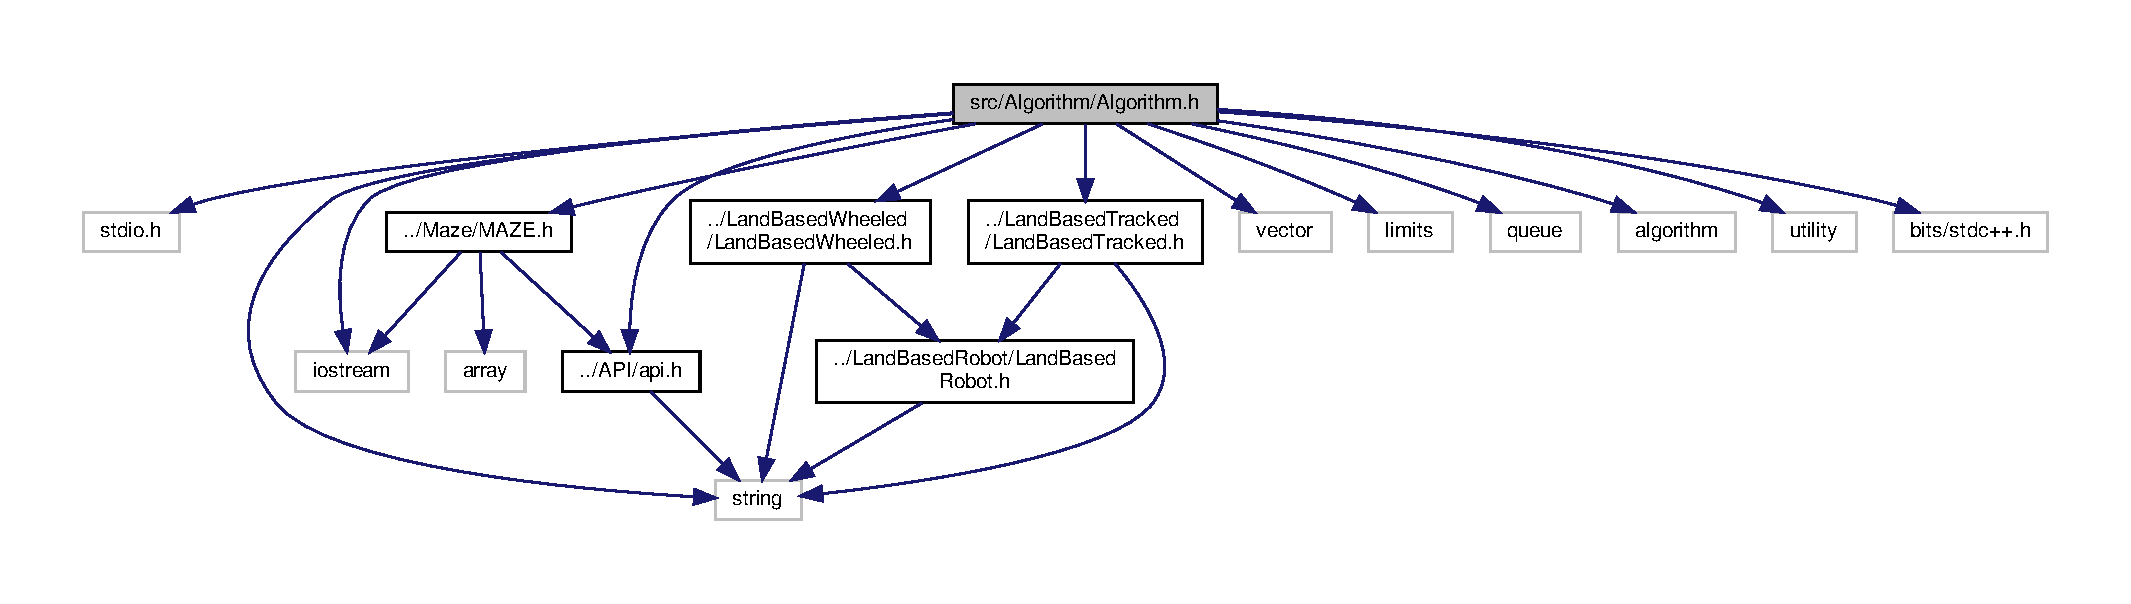
\includegraphics[width=350pt]{_algorithm_8h__incl}
\end{center}
\end{figure}
This graph shows which files directly or indirectly include this file\+:
\nopagebreak
\begin{figure}[H]
\begin{center}
\leavevmode
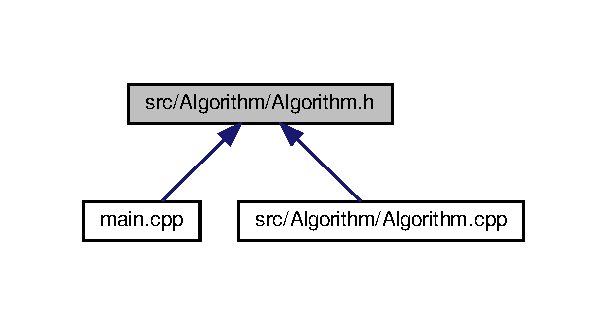
\includegraphics[width=292pt]{_algorithm_8h__dep__incl}
\end{center}
\end{figure}
\subsection*{Classes}
\begin{DoxyCompactItemize}
\item 
class \hyperlink{classfp_1_1_algorithm}{fp\+::\+Algorithm}
\end{DoxyCompactItemize}
\subsection*{Namespaces}
\begin{DoxyCompactItemize}
\item 
 \hyperlink{namespacefp}{fp}
\begin{DoxyCompactList}\small\item\em namespace from the base class \end{DoxyCompactList}\end{DoxyCompactItemize}


\subsection{Detailed Description}
Class to be used in source file and the functions that have been used. 

\begin{DoxyAuthor}{Author}
Group9 $<$\+E\+N\+P\+M809\+Y$>$ 
\end{DoxyAuthor}
\begin{DoxyVersion}{Version}
2.\+0
\end{DoxyVersion}
\hypertarget{_m_a_z_e_8h_LICENSE}{}\subsection{L\+I\+C\+E\+N\+SE}\label{_m_a_z_e_8h_LICENSE}
This program is free software; you can redistribute it and/or modify it under the terms of the G\+NU General Public License as published by the Free Software Foundation; either version 2 of the License, or (at your option) any later version.\hypertarget{_m_a_z_e_8h_DESCRIPTION}{}\subsection{D\+E\+S\+C\+R\+I\+P\+T\+I\+ON}\label{_m_a_z_e_8h_DESCRIPTION}
This C++ program is algorithm declaration for function to be used in source file for the maze. Applied algorithm is B\+F\+S(\+Brute(\+Breadth) Force Search). All the used files are declared here.\hypertarget{_m_a_z_e_8h_DESCRIPTION}{}\subsection{D\+E\+S\+C\+R\+I\+P\+T\+I\+ON}\label{_m_a_z_e_8h_DESCRIPTION}
This class declaration is the files to be used in the source file and the behaviour has been implemented in the source file 
\hypertarget{api_8cpp}{}\section{src/\+A\+P\+I/api.cpp File Reference}
\label{api_8cpp}\index{src/\+A\+P\+I/api.\+cpp@{src/\+A\+P\+I/api.\+cpp}}
{\ttfamily \#include \char`\"{}api.\+h\char`\"{}}\newline
{\ttfamily \#include $<$cstdlib$>$}\newline
{\ttfamily \#include $<$iostream$>$}\newline
Include dependency graph for api.\+cpp\+:
\nopagebreak
\begin{figure}[H]
\begin{center}
\leavevmode
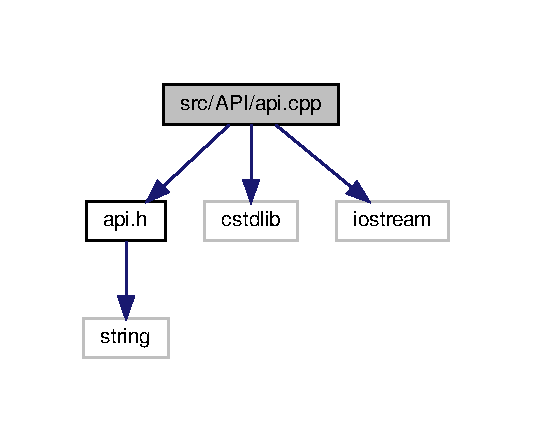
\includegraphics[width=256pt]{api_8cpp__incl}
\end{center}
\end{figure}


\subsection{Detailed Description}
\begin{DoxyAuthor}{Author}
Group9 $<$\+E\+N\+P\+M809\+Y$>$ 
\end{DoxyAuthor}
\begin{DoxyVersion}{Version}
2.\+0
\end{DoxyVersion}
\hypertarget{_m_a_z_e_8h_LICENSE}{}\subsection{L\+I\+C\+E\+N\+SE}\label{_m_a_z_e_8h_LICENSE}
This program is free software; you can redistribute it and/or modify it under the terms of the G\+NU General Public License as published by the Free Software Foundation; either version 2 of the License, or (at your option) any later version.\hypertarget{_m_a_z_e_8h_DESCRIPTION}{}\subsection{D\+E\+S\+C\+R\+I\+P\+T\+I\+ON}\label{_m_a_z_e_8h_DESCRIPTION}
This C++ program is A\+PI source files where robot moving functions have been defined. 
\hypertarget{api_8h}{}\section{src/\+A\+P\+I/api.h File Reference}
\label{api_8h}\index{src/\+A\+P\+I/api.\+h@{src/\+A\+P\+I/api.\+h}}


Class to be used in source file and the functions that have been used.  


{\ttfamily \#include $<$string$>$}\newline
Include dependency graph for api.\+h\+:
\nopagebreak
\begin{figure}[H]
\begin{center}
\leavevmode
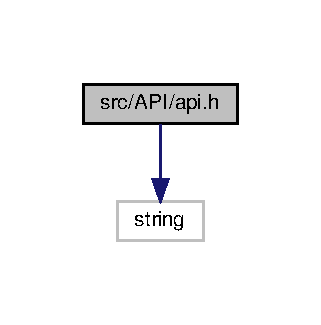
\includegraphics[width=154pt]{api_8h__incl}
\end{center}
\end{figure}
This graph shows which files directly or indirectly include this file\+:
\nopagebreak
\begin{figure}[H]
\begin{center}
\leavevmode
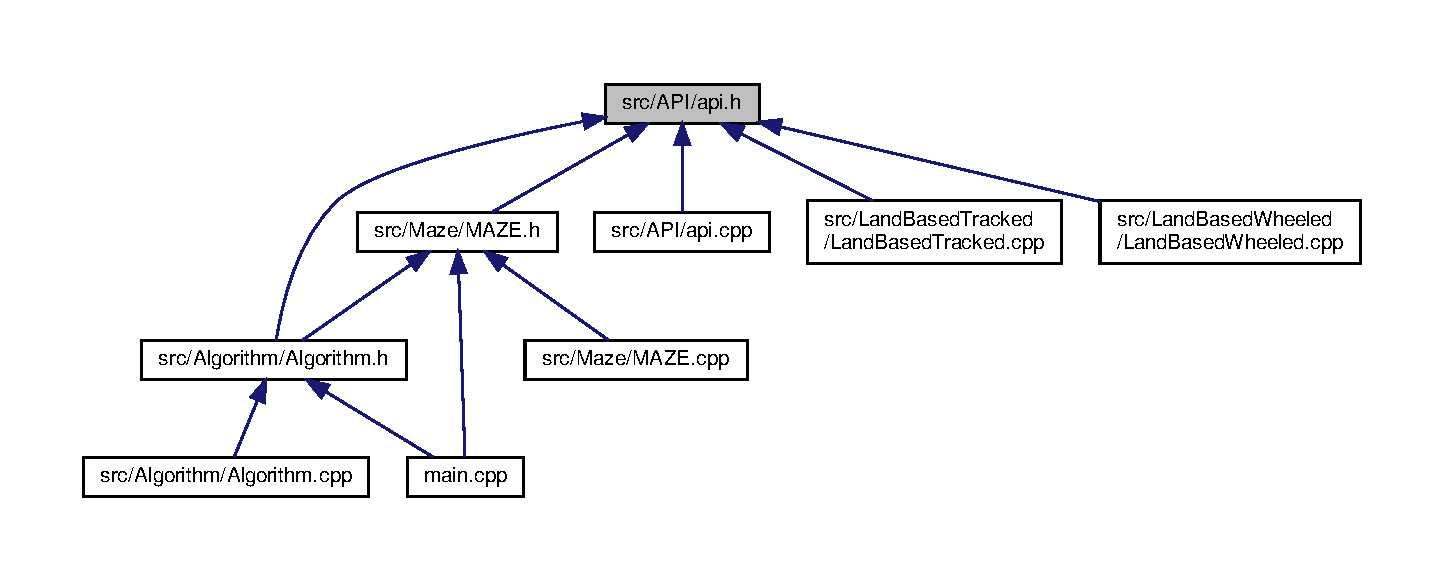
\includegraphics[width=350pt]{api_8h__dep__incl}
\end{center}
\end{figure}
\subsection*{Classes}
\begin{DoxyCompactItemize}
\item 
class \hyperlink{classfp_1_1_a_p_i}{fp\+::\+A\+PI}
\end{DoxyCompactItemize}
\subsection*{Namespaces}
\begin{DoxyCompactItemize}
\item 
 \hyperlink{namespacefp}{fp}
\begin{DoxyCompactList}\small\item\em namespace from the base class \end{DoxyCompactList}\end{DoxyCompactItemize}


\subsection{Detailed Description}
Class to be used in source file and the functions that have been used. 

\begin{DoxyAuthor}{Author}
Group9 $<$\+E\+N\+P\+M809\+Y$>$ 
\end{DoxyAuthor}
\begin{DoxyVersion}{Version}
2.\+0
\end{DoxyVersion}
\hypertarget{_m_a_z_e_8h_LICENSE}{}\subsection{L\+I\+C\+E\+N\+SE}\label{_m_a_z_e_8h_LICENSE}
This program is free software; you can redistribute it and/or modify it under the terms of the G\+NU General Public License as published by the Free Software Foundation; either version 2 of the License, or (at your option) any later version.\hypertarget{_m_a_z_e_8h_DESCRIPTION}{}\subsection{D\+E\+S\+C\+R\+I\+P\+T\+I\+ON}\label{_m_a_z_e_8h_DESCRIPTION}
This C++ program is A\+PI header files where we have declared variables and function used in cpp file to be used in source file for the maze. All the used files are declared here.\hypertarget{_m_a_z_e_8h_DESCRIPTION}{}\subsection{D\+E\+S\+C\+R\+I\+P\+T\+I\+ON}\label{_m_a_z_e_8h_DESCRIPTION}
This class declaration for files which are in \hyperlink{api_8cpp}{api.\+cpp} this all function will be used to move robot. 
\hypertarget{_land_based_robot_8cpp}{}\section{src/\+Land\+Based\+Robot/\+Land\+Based\+Robot.cpp File Reference}
\label{_land_based_robot_8cpp}\index{src/\+Land\+Based\+Robot/\+Land\+Based\+Robot.\+cpp@{src/\+Land\+Based\+Robot/\+Land\+Based\+Robot.\+cpp}}
{\ttfamily \#include \char`\"{}Land\+Based\+Robot.\+h\char`\"{}}\newline
{\ttfamily \#include $<$iostream$>$}\newline
Include dependency graph for Land\+Based\+Robot.\+cpp\+:
\nopagebreak
\begin{figure}[H]
\begin{center}
\leavevmode
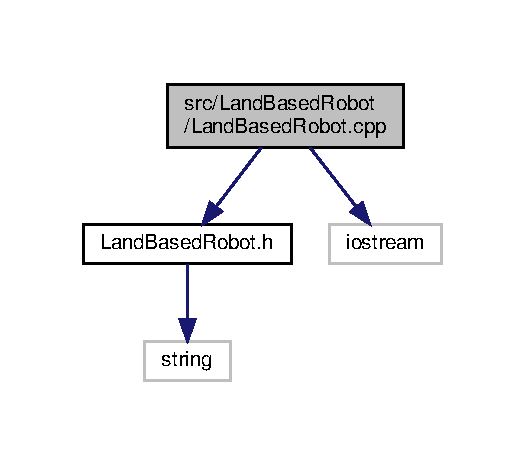
\includegraphics[width=252pt]{_land_based_robot_8cpp__incl}
\end{center}
\end{figure}


\subsection{Detailed Description}
\begin{DoxyAuthor}{Author}
Group9 $<$\+E\+N\+P\+M809\+Y$>$ 
\end{DoxyAuthor}
\begin{DoxyVersion}{Version}
2.\+0
\end{DoxyVersion}
\hypertarget{_m_a_z_e_8h_LICENSE}{}\subsection{L\+I\+C\+E\+N\+SE}\label{_m_a_z_e_8h_LICENSE}
This program is free software; you can redistribute it and/or modify it under the terms of the G\+NU General Public License as published by the Free Software Foundation; either version 2 of the License, or (at your option) any later version.\hypertarget{_m_a_z_e_8h_DESCRIPTION}{}\subsection{D\+E\+S\+C\+R\+I\+P\+T\+I\+ON}\label{_m_a_z_e_8h_DESCRIPTION}
This C++ program is a source file for the Land\+Based\+Robot. Here we have used all the function defined for the headerfile and just printed out that this particular function has been called. 
\hypertarget{_land_based_robot_8h}{}\section{src/\+Land\+Based\+Robot/\+Land\+Based\+Robot.h File Reference}
\label{_land_based_robot_8h}\index{src/\+Land\+Based\+Robot/\+Land\+Based\+Robot.\+h@{src/\+Land\+Based\+Robot/\+Land\+Based\+Robot.\+h}}


A file for base class inclusion.  


{\ttfamily \#include $<$string$>$}\newline
Include dependency graph for Land\+Based\+Robot.\+h\+:
\nopagebreak
\begin{figure}[H]
\begin{center}
\leavevmode
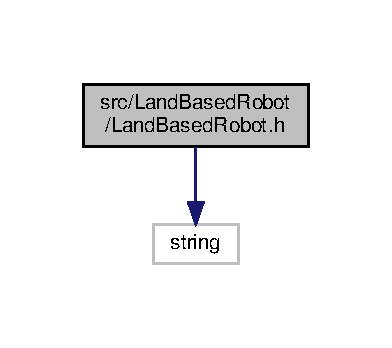
\includegraphics[width=188pt]{_land_based_robot_8h__incl}
\end{center}
\end{figure}
This graph shows which files directly or indirectly include this file\+:
\nopagebreak
\begin{figure}[H]
\begin{center}
\leavevmode
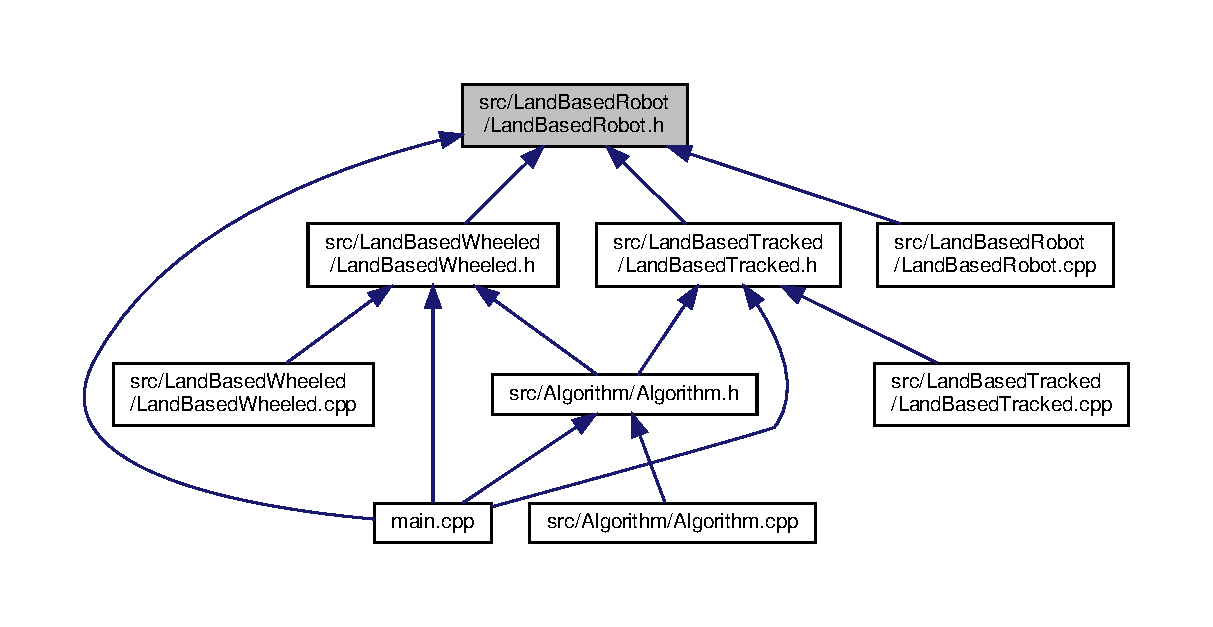
\includegraphics[width=350pt]{_land_based_robot_8h__dep__incl}
\end{center}
\end{figure}
\subsection*{Classes}
\begin{DoxyCompactItemize}
\item 
class \hyperlink{classfp_1_1_land_based_robot}{fp\+::\+Land\+Based\+Robot}
\end{DoxyCompactItemize}
\subsection*{Namespaces}
\begin{DoxyCompactItemize}
\item 
 \hyperlink{namespacefp}{fp}
\begin{DoxyCompactList}\small\item\em namespace from the base class \end{DoxyCompactList}\end{DoxyCompactItemize}


\subsection{Detailed Description}
A file for base class inclusion. 

Class to be used in source file and the functions that have been used.

A base class from which we inherit properties of Land\+Based\+Robots like Go\+Up and Go\+Down.

\begin{DoxyAuthor}{Author}
Group9 $<$\+E\+N\+P\+M809\+Y$>$ 
\end{DoxyAuthor}
\begin{DoxyVersion}{Version}
2.\+0
\end{DoxyVersion}
\hypertarget{_m_a_z_e_8h_LICENSE}{}\subsection{L\+I\+C\+E\+N\+SE}\label{_m_a_z_e_8h_LICENSE}
This program is free software; you can redistribute it and/or modify it under the terms of the G\+NU General Public License as published by the Free Software Foundation; either version 2 of the License, or (at your option) any later version.\hypertarget{_m_a_z_e_8h_DESCRIPTION}{}\subsection{D\+E\+S\+C\+R\+I\+P\+T\+I\+ON}\label{_m_a_z_e_8h_DESCRIPTION}
This C++ program is a header file for the Land\+Based\+Robot. This is an abstract base class from which we will inherit all the functions of base class like simple Go\+Up and Go\+Down and besides we also have access of attributes like speed and width as well.\hypertarget{_m_a_z_e_8h_DESCRIPTION}{}\subsection{D\+E\+S\+C\+R\+I\+P\+T\+I\+ON}\label{_m_a_z_e_8h_DESCRIPTION}
This class declaration for files which are in \hyperlink{_land_based_robot_8cpp}{Land\+Based\+Robot.\+cpp} this all function will be used to move robot.

A base class from which we inherit properties of Land\+Based\+Robots. 
\hypertarget{_land_based_tracked_8cpp}{}\section{src/\+Land\+Based\+Tracked/\+Land\+Based\+Tracked.cpp File Reference}
\label{_land_based_tracked_8cpp}\index{src/\+Land\+Based\+Tracked/\+Land\+Based\+Tracked.\+cpp@{src/\+Land\+Based\+Tracked/\+Land\+Based\+Tracked.\+cpp}}
{\ttfamily \#include \char`\"{}Land\+Based\+Tracked.\+h\char`\"{}}\newline
{\ttfamily \#include \char`\"{}../\+A\+P\+I/api.\+h\char`\"{}}\newline
{\ttfamily \#include $<$iostream$>$}\newline
{\ttfamily \#include $<$string$>$}\newline
Include dependency graph for Land\+Based\+Tracked.\+cpp\+:
\nopagebreak
\begin{figure}[H]
\begin{center}
\leavevmode
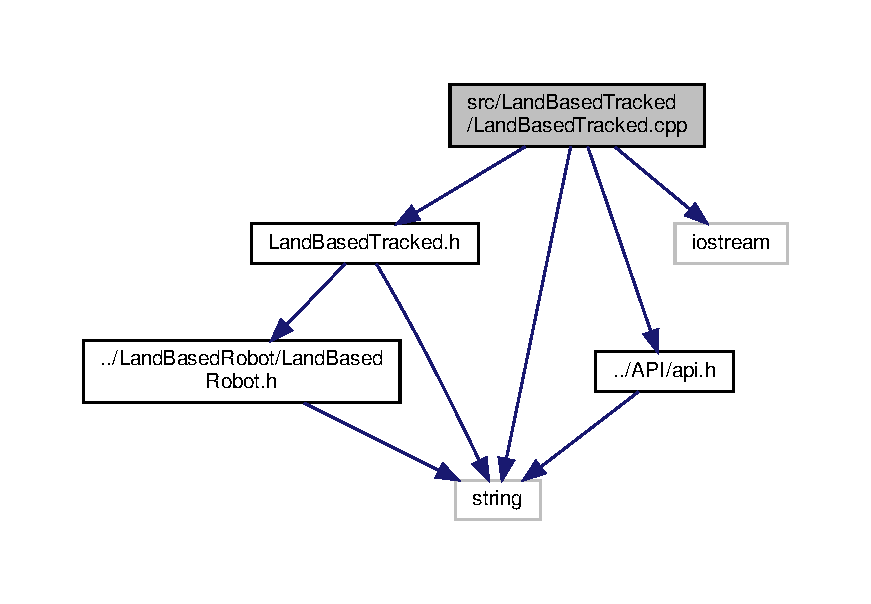
\includegraphics[width=350pt]{_land_based_tracked_8cpp__incl}
\end{center}
\end{figure}


\subsection{Detailed Description}
\begin{DoxyAuthor}{Author}
Group9 $<$\+E\+N\+P\+M809\+Y$>$ 
\end{DoxyAuthor}
\begin{DoxyVersion}{Version}
2.\+0
\end{DoxyVersion}
\hypertarget{_m_a_z_e_8h_LICENSE}{}\subsection{L\+I\+C\+E\+N\+SE}\label{_m_a_z_e_8h_LICENSE}
This program is free software; you can redistribute it and/or modify it under the terms of the G\+NU General Public License as published by the Free Software Foundation; either version 2 of the License, or (at your option) any later version.\hypertarget{_m_a_z_e_8h_DESCRIPTION}{}\subsection{D\+E\+S\+C\+R\+I\+P\+T\+I\+ON}\label{_m_a_z_e_8h_DESCRIPTION}
This C++ program is a source file for the Land\+Basedtracked robot. This implements derived class from the Landbased class and inherited all the valid function from it.\+The namespace is given as fp(a wrapped namespace for the whole base class) This has attributes protected attributes like track type. 
\hypertarget{_land_based_tracked_8h}{}\section{src/\+Land\+Based\+Tracked/\+Land\+Based\+Tracked.h File Reference}
\label{_land_based_tracked_8h}\index{src/\+Land\+Based\+Tracked/\+Land\+Based\+Tracked.\+h@{src/\+Land\+Based\+Tracked/\+Land\+Based\+Tracked.\+h}}


A file for base class inclusion.  


{\ttfamily \#include \char`\"{}../\+Land\+Based\+Robot/\+Land\+Based\+Robot.\+h\char`\"{}}\newline
{\ttfamily \#include $<$string$>$}\newline
Include dependency graph for Land\+Based\+Tracked.\+h\+:
\nopagebreak
\begin{figure}[H]
\begin{center}
\leavevmode
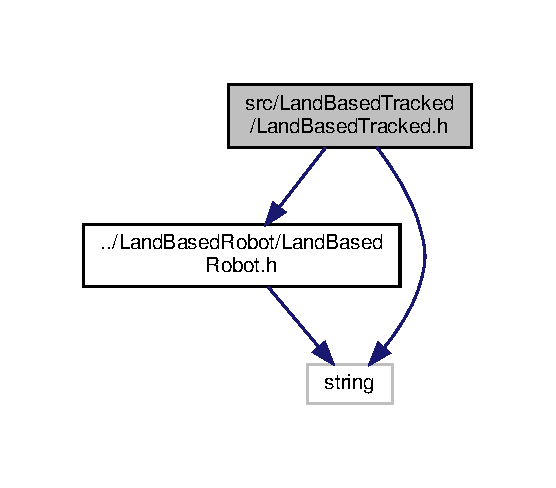
\includegraphics[width=267pt]{_land_based_tracked_8h__incl}
\end{center}
\end{figure}
This graph shows which files directly or indirectly include this file\+:
\nopagebreak
\begin{figure}[H]
\begin{center}
\leavevmode
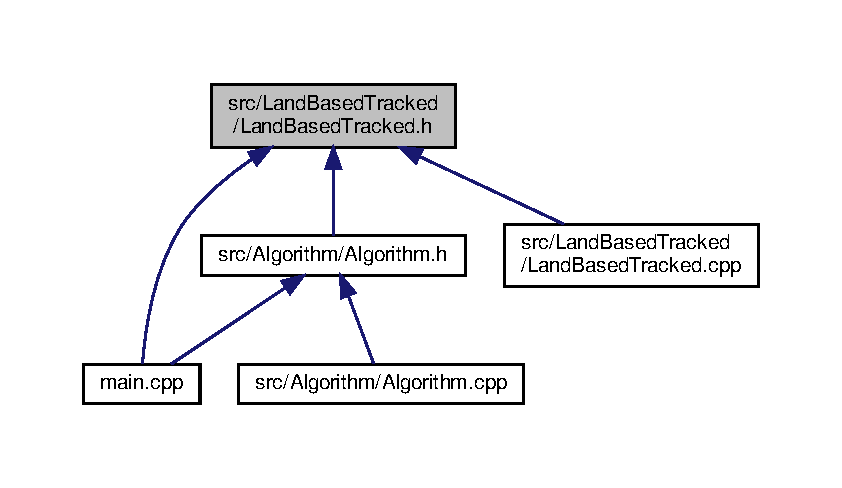
\includegraphics[width=350pt]{_land_based_tracked_8h__dep__incl}
\end{center}
\end{figure}
\subsection*{Classes}
\begin{DoxyCompactItemize}
\item 
class \hyperlink{classfp_1_1_land_based_tracked}{fp\+::\+Land\+Based\+Tracked}
\begin{DoxyCompactList}\small\item\em A Landbased\+Tracked class.. \end{DoxyCompactList}\end{DoxyCompactItemize}
\subsection*{Namespaces}
\begin{DoxyCompactItemize}
\item 
 \hyperlink{namespacefp}{fp}
\begin{DoxyCompactList}\small\item\em namespace from the base class \end{DoxyCompactList}\end{DoxyCompactItemize}


\subsection{Detailed Description}
A file for base class inclusion. 

A base class from which we inherit properties of Land\+Based\+Robot.

\begin{DoxyAuthor}{Author}
Group9 $<$\+E\+N\+P\+M809\+Y$>$ 
\end{DoxyAuthor}
\begin{DoxyVersion}{Version}
2.\+0
\end{DoxyVersion}
\hypertarget{_m_a_z_e_8h_LICENSE}{}\subsection{L\+I\+C\+E\+N\+SE}\label{_m_a_z_e_8h_LICENSE}
This program is free software; you can redistribute it and/or modify it under the terms of the G\+NU General Public License as published by the Free Software Foundation; either version 2 of the License, or (at your option) any later version.\hypertarget{_m_a_z_e_8h_DESCRIPTION}{}\subsection{D\+E\+S\+C\+R\+I\+P\+T\+I\+ON}\label{_m_a_z_e_8h_DESCRIPTION}
This C++ program is a header file for the Land\+Based\+Tracked robot. This is derived class from the Landbased class and inherited all the valid function from it.\+The namespace is given as fp(a wrapped namespace for the whole base class) This has attributes protected attributes like track type. 
\hypertarget{_land_based_wheeled_8cpp}{}\section{src/\+Land\+Based\+Wheeled/\+Land\+Based\+Wheeled.cpp File Reference}
\label{_land_based_wheeled_8cpp}\index{src/\+Land\+Based\+Wheeled/\+Land\+Based\+Wheeled.\+cpp@{src/\+Land\+Based\+Wheeled/\+Land\+Based\+Wheeled.\+cpp}}
{\ttfamily \#include \char`\"{}Land\+Based\+Wheeled.\+h\char`\"{}}\newline
{\ttfamily \#include \char`\"{}../\+A\+P\+I/api.\+h\char`\"{}}\newline
{\ttfamily \#include $<$iostream$>$}\newline
{\ttfamily \#include $<$string$>$}\newline
Include dependency graph for Land\+Based\+Wheeled.\+cpp\+:
\nopagebreak
\begin{figure}[H]
\begin{center}
\leavevmode
\includegraphics[width=350pt]{_land_based_wheeled_8cpp__incl}
\end{center}
\end{figure}


\subsection{Detailed Description}
\begin{DoxyAuthor}{Author}
Group9 $<$\+E\+N\+P\+M809\+Y$>$ 
\end{DoxyAuthor}
\begin{DoxyVersion}{Version}
2.\+0
\end{DoxyVersion}
\hypertarget{_m_a_z_e_8h_LICENSE}{}\subsection{L\+I\+C\+E\+N\+SE}\label{_m_a_z_e_8h_LICENSE}
This program is free software; you can redistribute it and/or modify it under the terms of the G\+NU General Public License as published by the Free Software Foundation; either version 2 of the License, or (at your option) any later version.\hypertarget{_m_a_z_e_8h_DESCRIPTION}{}\subsection{D\+E\+S\+C\+R\+I\+P\+T\+I\+ON}\label{_m_a_z_e_8h_DESCRIPTION}
This C++ program is a source file for the Land\+Based\+Wheeled robot. This implements derived class from the Landbased class and inherited all the valid function from it.\+The namespace is given as fp(a wrapped namespace for the whole base class) This has attributes protected attributes like wheel number and wheel type. 
\hypertarget{_land_based_wheeled_8h}{}\section{src/\+Land\+Based\+Wheeled/\+Land\+Based\+Wheeled.h File Reference}
\label{_land_based_wheeled_8h}\index{src/\+Land\+Based\+Wheeled/\+Land\+Based\+Wheeled.\+h@{src/\+Land\+Based\+Wheeled/\+Land\+Based\+Wheeled.\+h}}


A file for base class inclusion.  


{\ttfamily \#include \char`\"{}../\+Land\+Based\+Robot/\+Land\+Based\+Robot.\+h\char`\"{}}\newline
{\ttfamily \#include $<$string$>$}\newline
Include dependency graph for Land\+Based\+Wheeled.\+h\+:
\nopagebreak
\begin{figure}[H]
\begin{center}
\leavevmode
\includegraphics[width=268pt]{_land_based_wheeled_8h__incl}
\end{center}
\end{figure}
This graph shows which files directly or indirectly include this file\+:
\nopagebreak
\begin{figure}[H]
\begin{center}
\leavevmode
\includegraphics[width=350pt]{_land_based_wheeled_8h__dep__incl}
\end{center}
\end{figure}
\subsection*{Classes}
\begin{DoxyCompactItemize}
\item 
class \hyperlink{classfp_1_1_land_based_wheeled}{fp\+::\+Land\+Based\+Wheeled}
\begin{DoxyCompactList}\small\item\em A Landbased\+Wheeled class.. \end{DoxyCompactList}\end{DoxyCompactItemize}
\subsection*{Namespaces}
\begin{DoxyCompactItemize}
\item 
 \hyperlink{namespacefp}{fp}
\begin{DoxyCompactList}\small\item\em namespace from the base class \end{DoxyCompactList}\end{DoxyCompactItemize}


\subsection{Detailed Description}
A file for base class inclusion. 

A base class from which we inherit properties of Land\+Based\+Robot.

\begin{DoxyAuthor}{Author}
Group9 $<$\+E\+N\+P\+M809\+Y$>$ 
\end{DoxyAuthor}
\begin{DoxyVersion}{Version}
2.\+0
\end{DoxyVersion}
\hypertarget{_m_a_z_e_8h_LICENSE}{}\subsection{L\+I\+C\+E\+N\+SE}\label{_m_a_z_e_8h_LICENSE}
This program is free software; you can redistribute it and/or modify it under the terms of the G\+NU General Public License as published by the Free Software Foundation; either version 2 of the License, or (at your option) any later version.\hypertarget{_m_a_z_e_8h_DESCRIPTION}{}\subsection{D\+E\+S\+C\+R\+I\+P\+T\+I\+ON}\label{_m_a_z_e_8h_DESCRIPTION}
This C++ program is a header file for the Land\+Based\+Wheeled robot. This is derived class from the Landbased class and inherited all the valid function from it.\+The namespace is given as fp(a wrapped namespace for the whole base class) This has attributes protected attributes like wheel number and wheel type. 
\hypertarget{_m_a_z_e_8cpp}{}\section{src/\+Maze/\+M\+A\+ZE.cpp File Reference}
\label{_m_a_z_e_8cpp}\index{src/\+Maze/\+M\+A\+Z\+E.\+cpp@{src/\+Maze/\+M\+A\+Z\+E.\+cpp}}
{\ttfamily \#include $<$iostream$>$}\newline
{\ttfamily \#include \char`\"{}M\+A\+Z\+E.\+h\char`\"{}}\newline
Include dependency graph for M\+A\+Z\+E.\+cpp\+:
\nopagebreak
\begin{figure}[H]
\begin{center}
\leavevmode
\includegraphics[width=274pt]{_m_a_z_e_8cpp__incl}
\end{center}
\end{figure}


\subsection{Detailed Description}
\begin{DoxyAuthor}{Author}
Group9 $<$\+E\+N\+P\+M809\+Y$>$ 
\end{DoxyAuthor}
\begin{DoxyVersion}{Version}
2.\+0
\end{DoxyVersion}
\hypertarget{_m_a_z_e_8h_LICENSE}{}\subsection{L\+I\+C\+E\+N\+SE}\label{_m_a_z_e_8h_LICENSE}
This program is free software; you can redistribute it and/or modify it under the terms of the G\+NU General Public License as published by the Free Software Foundation; either version 2 of the License, or (at your option) any later version.\hypertarget{_m_a_z_e_8h_DESCRIPTION}{}\subsection{D\+E\+S\+C\+R\+I\+P\+T\+I\+ON}\label{_m_a_z_e_8h_DESCRIPTION}
This C++ program is maze implementation for the maze Class and functions to be used are already declared in header file and other library have been included in header files. 
\hypertarget{_m_a_z_e_8h}{}\section{src/\+Maze/\+M\+A\+ZE.h File Reference}
\label{_m_a_z_e_8h}\index{src/\+Maze/\+M\+A\+Z\+E.\+h@{src/\+Maze/\+M\+A\+Z\+E.\+h}}


class declarartion with functions wrapped in the namespace fp.  


{\ttfamily \#include $<$iostream$>$}\newline
{\ttfamily \#include $<$array$>$}\newline
{\ttfamily \#include \char`\"{}../\+A\+P\+I/api.\+h\char`\"{}}\newline
Include dependency graph for M\+A\+Z\+E.\+h\+:
\nopagebreak
\begin{figure}[H]
\begin{center}
\leavevmode
\includegraphics[width=274pt]{_m_a_z_e_8h__incl}
\end{center}
\end{figure}
This graph shows which files directly or indirectly include this file\+:
\nopagebreak
\begin{figure}[H]
\begin{center}
\leavevmode
\includegraphics[width=350pt]{_m_a_z_e_8h__dep__incl}
\end{center}
\end{figure}
\subsection*{Classes}
\begin{DoxyCompactItemize}
\item 
class \hyperlink{classfp_1_1_maze}{fp\+::\+Maze}
\end{DoxyCompactItemize}
\subsection*{Namespaces}
\begin{DoxyCompactItemize}
\item 
 \hyperlink{namespacefp}{fp}
\begin{DoxyCompactList}\small\item\em namespace from the base class \end{DoxyCompactList}\end{DoxyCompactItemize}


\subsection{Detailed Description}
class declarartion with functions wrapped in the namespace fp. 

\begin{DoxyAuthor}{Author}
Group9 $<$\+E\+N\+P\+M809\+Y$>$ 
\end{DoxyAuthor}
\begin{DoxyVersion}{Version}
2.\+0
\end{DoxyVersion}
\hypertarget{_m_a_z_e_8h_LICENSE}{}\subsection{L\+I\+C\+E\+N\+SE}\label{_m_a_z_e_8h_LICENSE}
This program is free software; you can redistribute it and/or modify it under the terms of the G\+NU General Public License as published by the Free Software Foundation; either version 2 of the License, or (at your option) any later version.\hypertarget{_m_a_z_e_8h_DESCRIPTION}{}\subsection{D\+E\+S\+C\+R\+I\+P\+T\+I\+ON}\label{_m_a_z_e_8h_DESCRIPTION}
This C++ program is amaze class declaration for the maze. Class and functions to be used are are declared in header file and other library have been included in this header file.
%--- End generated contents ---

% Index
\backmatter
\newpage
\phantomsection
\clearemptydoublepage
\addcontentsline{toc}{chapter}{Index}
\printindex

\end{document}
